\PassOptionsToPackage{unicode=true}{hyperref} % options for packages loaded elsewhere
\PassOptionsToPackage{hyphens}{url}
%
\documentclass[12pt,]{style/krantz}
\usepackage{lmodern}
\usepackage{amssymb,amsmath}
\usepackage{ifxetex,ifluatex}
\usepackage{fixltx2e} % provides \textsubscript
\ifnum 0\ifxetex 1\fi\ifluatex 1\fi=0 % if pdftex
  \usepackage[T1]{fontenc}
  \usepackage[utf8]{inputenc}
  \usepackage{textcomp} % provides euro and other symbols
\else % if luatex or xelatex
  \usepackage{unicode-math}
  \defaultfontfeatures{Ligatures=TeX,Scale=MatchLowercase}
    \setmonofont[Mapping=tex-ansi,Scale=0.7]{Source Code Pro}
\fi
% use upquote if available, for straight quotes in verbatim environments
\IfFileExists{upquote.sty}{\usepackage{upquote}}{}
% use microtype if available
\IfFileExists{microtype.sty}{%
\usepackage[]{microtype}
\UseMicrotypeSet[protrusion]{basicmath} % disable protrusion for tt fonts
}{}
\IfFileExists{parskip.sty}{%
\usepackage{parskip}
}{% else
\setlength{\parindent}{0pt}
\setlength{\parskip}{6pt plus 2pt minus 1pt}
}
\usepackage{hyperref}
\hypersetup{
            pdftitle={R NA PRÁTICA: Estatística Descomplicada com R},
            pdfauthor={José Evandeilton lopes},
            pdfborder={0 0 0},
            breaklinks=true}
\urlstyle{same}  % don't use monospace font for urls
\usepackage{color}
\usepackage{fancyvrb}
\newcommand{\VerbBar}{|}
\newcommand{\VERB}{\Verb[commandchars=\\\{\}]}
\DefineVerbatimEnvironment{Highlighting}{Verbatim}{commandchars=\\\{\}}
% Add ',fontsize=\small' for more characters per line
\usepackage{framed}
\definecolor{shadecolor}{RGB}{248,248,248}
\newenvironment{Shaded}{\begin{snugshade}}{\end{snugshade}}
\newcommand{\AlertTok}[1]{\textcolor[rgb]{0.94,0.16,0.16}{#1}}
\newcommand{\AnnotationTok}[1]{\textcolor[rgb]{0.56,0.35,0.01}{\textbf{\textit{#1}}}}
\newcommand{\AttributeTok}[1]{\textcolor[rgb]{0.77,0.63,0.00}{#1}}
\newcommand{\BaseNTok}[1]{\textcolor[rgb]{0.00,0.00,0.81}{#1}}
\newcommand{\BuiltInTok}[1]{#1}
\newcommand{\CharTok}[1]{\textcolor[rgb]{0.31,0.60,0.02}{#1}}
\newcommand{\CommentTok}[1]{\textcolor[rgb]{0.56,0.35,0.01}{\textit{#1}}}
\newcommand{\CommentVarTok}[1]{\textcolor[rgb]{0.56,0.35,0.01}{\textbf{\textit{#1}}}}
\newcommand{\ConstantTok}[1]{\textcolor[rgb]{0.00,0.00,0.00}{#1}}
\newcommand{\ControlFlowTok}[1]{\textcolor[rgb]{0.13,0.29,0.53}{\textbf{#1}}}
\newcommand{\DataTypeTok}[1]{\textcolor[rgb]{0.13,0.29,0.53}{#1}}
\newcommand{\DecValTok}[1]{\textcolor[rgb]{0.00,0.00,0.81}{#1}}
\newcommand{\DocumentationTok}[1]{\textcolor[rgb]{0.56,0.35,0.01}{\textbf{\textit{#1}}}}
\newcommand{\ErrorTok}[1]{\textcolor[rgb]{0.64,0.00,0.00}{\textbf{#1}}}
\newcommand{\ExtensionTok}[1]{#1}
\newcommand{\FloatTok}[1]{\textcolor[rgb]{0.00,0.00,0.81}{#1}}
\newcommand{\FunctionTok}[1]{\textcolor[rgb]{0.00,0.00,0.00}{#1}}
\newcommand{\ImportTok}[1]{#1}
\newcommand{\InformationTok}[1]{\textcolor[rgb]{0.56,0.35,0.01}{\textbf{\textit{#1}}}}
\newcommand{\KeywordTok}[1]{\textcolor[rgb]{0.13,0.29,0.53}{\textbf{#1}}}
\newcommand{\NormalTok}[1]{#1}
\newcommand{\OperatorTok}[1]{\textcolor[rgb]{0.81,0.36,0.00}{\textbf{#1}}}
\newcommand{\OtherTok}[1]{\textcolor[rgb]{0.56,0.35,0.01}{#1}}
\newcommand{\PreprocessorTok}[1]{\textcolor[rgb]{0.56,0.35,0.01}{\textit{#1}}}
\newcommand{\RegionMarkerTok}[1]{#1}
\newcommand{\SpecialCharTok}[1]{\textcolor[rgb]{0.00,0.00,0.00}{#1}}
\newcommand{\SpecialStringTok}[1]{\textcolor[rgb]{0.31,0.60,0.02}{#1}}
\newcommand{\StringTok}[1]{\textcolor[rgb]{0.31,0.60,0.02}{#1}}
\newcommand{\VariableTok}[1]{\textcolor[rgb]{0.00,0.00,0.00}{#1}}
\newcommand{\VerbatimStringTok}[1]{\textcolor[rgb]{0.31,0.60,0.02}{#1}}
\newcommand{\WarningTok}[1]{\textcolor[rgb]{0.56,0.35,0.01}{\textbf{\textit{#1}}}}
\usepackage{longtable,booktabs}
% Fix footnotes in tables (requires footnote package)
\IfFileExists{footnote.sty}{\usepackage{footnote}\makesavenoteenv{longtable}}{}
\setlength{\emergencystretch}{3em}  % prevent overfull lines
\providecommand{\tightlist}{%
  \setlength{\itemsep}{0pt}\setlength{\parskip}{0pt}}
\setcounter{secnumdepth}{5}
% Redefines (sub)paragraphs to behave more like sections
\ifx\paragraph\undefined\else
\let\oldparagraph\paragraph
\renewcommand{\paragraph}[1]{\oldparagraph{#1}\mbox{}}
\fi
\ifx\subparagraph\undefined\else
\let\oldsubparagraph\subparagraph
\renewcommand{\subparagraph}[1]{\oldsubparagraph{#1}\mbox{}}
\fi

% set default figure placement to htbp
\makeatletter
\def\fps@figure{htbp}
\makeatother

\usepackage{booktabs}
\usepackage{longtable}
\usepackage[bf,singlelinecheck=off]{caption}

%Edit JEL
\usepackage{float}
\usepackage{graphicx}
%\usepackage[default]{sourcesanspro}
%\usepackage[T1]{fontenc}
%\graphicspath{ {../Imagens} }
% ---------------

\usepackage{framed,color}
\definecolor{shadecolor}{RGB}{248,248,248}

\renewcommand{\textfraction}{0.05}
\renewcommand{\topfraction}{0.8}
\renewcommand{\bottomfraction}{0.8}
\renewcommand{\floatpagefraction}{0.75}

\renewenvironment{quote}{\begin{VF}}{\end{VF}}
\let\oldhref\href
\renewcommand{\href}[2]{#2\footnote{\url{#1}}}

% \ifxetex
  % \usepackage{letltxmacro}
  % \setlength{\XeTeXLinkMargin}{1pt}
  % \LetLtxMacro\SavedIncludeGraphics\includegraphics
  % \def\includegraphics#1#{% #1 catches optional stuff (star/opt. arg.)
    % \IncludeGraphicsAux{#1}%
  % }%
  % \newcommand*{\IncludeGraphicsAux}[2]{%
    % \XeTeXLinkBox{%
      % \SavedIncludeGraphics#1{#2}%
    % }%
  % }%
% \fi

\makeatletter
\newenvironment{kframe}{%
\medskip{}
\setlength{\fboxsep}{.8em}
 \def\at@end@of@kframe{}%
 \ifinner\ifhmode%
  \def\at@end@of@kframe{\end{minipage}}%
  \begin{minipage}{\columnwidth}%
 \fi\fi%
 \def\FrameCommand##1{\hskip\@totalleftmargin \hskip-\fboxsep
 \colorbox{shadecolor}{##1}\hskip-\fboxsep
     % There is no \\@totalrightmargin, so:
     \hskip-\linewidth \hskip-\@totalleftmargin \hskip\columnwidth}%
 \MakeFramed {\advance\hsize-\width
   \@totalleftmargin\z@ \linewidth\hsize
   \@setminipage}}%
 {\par\unskip\endMakeFramed%
 \at@end@of@kframe}
\makeatother

\renewenvironment{Shaded}{\begin{kframe}}{\end{kframe}}

\usepackage{makeidx}
\makeindex

\urlstyle{tt}

\usepackage{amsthm}
\makeatletter
\def\thm@space@setup{%
  \thm@preskip=8pt plus 2pt minus 4pt
  \thm@postskip=\thm@preskip
}
\makeatother

\frontmatter
\usepackage[]{natbib}
\bibliographystyle{apalike}

\title{R NA PRÁTICA: Estatística Descomplicada com R}
\author{José Evandeilton lopes}
\date{2019-02-28}

\usepackage{amsthm}
\newtheorem{theorem}{Teorema}[chapter]
\newtheorem{lemma}{Lema}[chapter]
\newtheorem{corollary}{Corolário}[chapter]
\newtheorem{proposition}{Proposição}[chapter]
\newtheorem{conjecture}{Conjectura}[chapter]
\theoremstyle{definition}
\newtheorem{definition}{Definição}[chapter]
\theoremstyle{definition}
\newtheorem{example}{Exemplo}[chapter]
\theoremstyle{definition}
\newtheorem{exercise}{Exercício}[chapter]
\theoremstyle{remark}
\newtheorem*{remark}{Nota}
\newtheorem*{solution}{Solução}
\let\BeginKnitrBlock\begin \let\EndKnitrBlock\end
\begin{document}
\maketitle

% you may need to leave a few empty pages before the dedication page

%\cleardoublepage\newpage\thispagestyle{empty}\null
%\cleardoublepage\newpage\thispagestyle{empty}\null
%\cleardoublepage\newpage
\thispagestyle{empty}

\begin{center}
To my son,

without whom I should have finished this book two years earlier
%\includegraphics{images/dedication.pdf}
\end{center}

\setlength{\abovedisplayskip}{-5pt}
\setlength{\abovedisplayshortskip}{-5pt}

{
\setcounter{tocdepth}{2}
\tableofcontents
}
\listoftables
\listoffigures
\hypertarget{introducao}{%
\chapter*{Introdução}\label{introducao}}


Bem vindo ao módulo I de Estatística descomplicada com o R NA PRÁTICA. Este é o primeiro módulo desta série de quatro módulos e contem pará os principais conceitos estatísticos até análise descritiva. O objetivo maior desta parte é revisar os conceitos mais importantes do inicio dos estudos estatísticos. Abordaremos a parte conceitual com algumas definições e termos estatísticos, tabelas de frequências, bem como as principais medidas descritivas (média, mediana e outras). Veremos por fim, os principais gráficos estatísticos mais utilizados. Para reforçar os conhecimentos, faremos muitos exercícios práticos com apoio do R com foco em bases de dados reais do \href{http://portal.inep.gov.br/web/guest/dados}{INEP} - Instituto Nacional de Estudos e Pesquisas Educacionais Anísio Teixeira do ano de 2017.

No final deste módulo você será capaz de:

\begin{itemize}
\tightlist
\item
  Definir estatística;
\item
  Compreender os principais tipos de variáveis;
\item
  Entender o que é e como utilizar tabelas de frequências;
\item
  Trabalhar com as principais medidas estatísticas (media, mediana, desvio padrão, etc.);
\item
  Entender correlação e covariância;
\item
  Construir gráficos estatísticos para os tipos corretas de dados.
\end{itemize}

\hypertarget{motivacao}{%
\section*{Motivação}\label{motivacao}}


A Estatística está em tudo! É atribuída a \href{https://www.sciencedirect.com/science/article/pii/0315086079901010}{H.G. Wells} a seguinte frase:

\begin{quote}
``Statistical thinking will one day be as necessary for efficient citizenship as the ability to read and write. --- H.G. Wells''
\end{quote}

Que em português se traduz em algo como:

\begin{quote}
``O conhecimento estatístico um dia será tão necessário para uma cidadania eficiente quanto a habilidade de ler e escrever.''
\end{quote}

Veja alguns exemplos de onde a estatística pode ser aplicada:

\begin{itemize}
\item
  \textbf{Na sua lista de compras:} Sim, é importante medir as diferenças de preços dos produtos e o percentual de seu salário gasto com alimentos pra não ficar sem grana por aluguel;
\item
  \textbf{Na previsão do tempo:} Sair sem guarda-chuva ou de bicicleta num dia de chuva, nem pensar. Mas você não saberia o que fazer pela manhã se observasse o dia claro e sem sinais de chuva. Somente uma previsão estatística confiável seria capaz de te ajudar a decidir antecipadamente;
\item
  \textbf{Na pesquisa científica:} Toda pesquisa científica usa estatística. Se não utilizar é porque não é científica mas sim, especulativa;
\item
  \textbf{Em seguros:} Seguros de vida, de veículos, de saúde, dental, daquele \href{https://www.moneytips.com/how-much-is-my-butt-worth}{bumbum siliconado}. Tudo envolve estatística. É através dela que os estatísticos constroem os melhores modelos com base em variáveis históricas e nas segmentações de perfis de cada grupo de indivíduos;
\item
  \textbf{Em pesquisas médicas:} Controle de epidemias, vacinas, taxas de sobrevida, taxas de recuperação de tecidos e ossos, regressão de doenças infecciosas, testes de grupos de risco e uma infinidade de situações utilizam estatística para prever, aumentar e melhorar processos que trazem ganho para a saúde e vida das pessoas;
\item
  \textbf{Em testes de qualidade:} A estatística bate forte na hora de uma empresa obter uma certificação ISO. Seja no controle estatístico de processos, gráficos de controle e/ou gestão da qualidade, sem esta ciência estes nichos não teriam os mesmos resultados;
\item
  \textbf{No monitoramento de ataques de vírus:} A empresa Kaspesrki por exemplo, coleta dados globais de vírus e sintetiza em um mapa do globo virtual denominado \href{https://cybermap.kaspersky.com/pt}{cybermap}. Através dele o usuário pode navegar e obter estatísticas relevantes sobre atividades de vírus nos países pelo mundo.
\item
  \textbf{No IDH e expectativa de vida:} O IDH (Índice de Desenvolvimento Humano) de um país é um bom indicador de desenvolvimento do mesmo. Não tem como calcular IDH sem modelos estatísticos.
\end{itemize}

\hypertarget{prerequisitos}{%
\section*{Prerequisitos}\label{prerequisitos}}


Para fazer o melhor proveito deste material, temos as seguintes recomendações:

\begin{itemize}
\tightlist
\item
  Tenha um computador com acesso á internet para poder assistir aos vídeos, fazer pesquisa e download dos materiais do curso;
\item
  Dedique pelo menos 2 horas da sua semana para ler o material e resolver os exercícios propostos;
\item
  Sempre que alguma dúvida surgir e não conseguir resolver com ajuda do material, contatar o professor via plataforma para obter suporte adicional;
\item
  Algum conhecimento prévio da linguagem R ou lógica de programação.
\end{itemize}

\hypertarget{ambiente-de-trabalho}{%
\section*{Ambiente de trabalho}\label{ambiente-de-trabalho}}


Este curso não tem a intenção de ensinar detalhadamente programação em R, pois o foco é em estatística. Contudo, sempre que necessário explicaremos algumas funções e comandos utilizados nos scripts. Além disso, para todos os exemplos e exercícios, deixaremos os códigos gerados como forma de estudo e revisão para que tudo possa ser replicado pelo aluno.

Se você sentir dificuldade em compreender algum conceito em linguagem R, recomendamos fazer o nosso curso \href{https://www.udemy.com/r-na-pratica-ciencia-de-dados/learn/v4/overview}{R NA PRÁTICA: Data Wrangling com R para Ciência de Dados} ou qualquer outro do seu interesse para obter mais conhecimentos dobre a linguagem R.

\hypertarget{pacotes}{%
\subsection*{Pacotes}\label{pacotes}}


Trabalharemos sempre que possível com o operador \texttt{\%\textgreater{}\%\ (pipe)} e com funções dos pacotes do \href{https://www.tidyverse.org/}{\texttt{tidyverse}} e outros relacionados.

Trabalharemos com o \href{https://cloud.r-project.org/}{software R} e com a IDE (Ambiente de Desenvolvimento Integrado, traduzindo do inglês) de desenvolvimento em R \href{https://www.rstudio.com/products/rstudio/download/\#download}{RStudio Desktop}. Nos links você poderá baixar os dois programas e configurar de acordo com o seu sistema operacional.

Especialmente para o R NA PRÁTICA, desenvolvemos o pacote \texttt{rnp} que poderá ser baixado direto to \texttt{github}. Este pacote possui recursos deste livro e também de outros materiais do R NA PRÁTICA.
Rode o comando abaixo para instalar, caso ainda não tenha o pacote.

\begin{Shaded}
\begin{Highlighting}[]
\KeywordTok{require}\NormalTok{(devtools, }\DataTypeTok{quietly =} \OtherTok{TRUE}\NormalTok{)}
\ControlFlowTok{if}\NormalTok{(}\OperatorTok{!}\KeywordTok{require}\NormalTok{(}\StringTok{"rnp"}\NormalTok{)) \{}
\NormalTok{ devtools}\OperatorTok{::}\KeywordTok{install_github}\NormalTok{(}\StringTok{"evandeilton/rnp"}\NormalTok{) }
\NormalTok{\}}
\end{Highlighting}
\end{Shaded}

Não nos restringimos apenas a este, remendamos caso ainda não tenha, instalar os pacotes listados a seguir:

\begin{Shaded}
\begin{Highlighting}[]
\NormalTok{pacotes <-}\StringTok{ }\KeywordTok{c}\NormalTok{(}\StringTok{"tidyverse"}\NormalTok{,}\StringTok{"lubridate"}\NormalTok{, }\StringTok{"magrittr"}\NormalTok{,}\StringTok{"broom"}\NormalTok{,}
             \StringTok{"stringr"}\NormalTok{, }\StringTok{"plotly"}\NormalTok{, }\StringTok{"ggplot2"}\NormalTok{,}\StringTok{"data.table"}\NormalTok{)}
\ControlFlowTok{for}\NormalTok{(i }\ControlFlowTok{in}\NormalTok{ pacotes)\{}
  \ControlFlowTok{if}\NormalTok{(}\OperatorTok{!}\KeywordTok{require}\NormalTok{(}\DataTypeTok{package =}\NormalTok{ i, }\DataTypeTok{character.only =} \OtherTok{TRUE}\NormalTok{))\{}
    \KeywordTok{install.packages}\NormalTok{(i, }\DataTypeTok{dependencies =} \OtherTok{TRUE}\NormalTok{)}
\NormalTok{  \}}
\NormalTok{\}}
\end{Highlighting}
\end{Shaded}

\hypertarget{conjuntos-de-dados}{%
\subsection*{Conjuntos de dados}\label{conjuntos-de-dados}}


Trabalharemos com conjuntos de dados do Censo do Ensino Superior no Brasil feito anualmente pelo \href{www.inep.gov.br/}{INEP (Instituto Nacional de Estudos e Pesquisas Educacionais Anísio Teixeira)}, especificamente para o ano de 2017. Os dados podem ser baixados diretamente na seção de microdados do site neste link \href{http://portal.inep.gov.br/microdados}{Censo da Educação Superior de 2017}, ou se preferir, baixar diretamente com o comando abaixo. Em seguinda descompactar os dados utilizando seu descompactador favorito.

\begin{Shaded}
\begin{Highlighting}[]
\CommentTok{# Informa o ano dos dados e o local completo de onde deseja salvar os dados}
\CommentTok{# conforme exemplos abaixo. Recomendamos criar uma pasta para salvar os}
\CommentTok{# dados e tornar mais acessíveis nas aulas.}
\NormalTok{rnp}\OperatorTok{::}\KeywordTok{rnp_get_inep_censo}\NormalTok{(}\DataTypeTok{ano =} \DecValTok{2017}\NormalTok{, }\DataTypeTok{salvar =} \StringTok{"Dados/INEP/"}\NormalTok{)}
\end{Highlighting}
\end{Shaded}

Você poderá também ler os dados sem decompactar com o pacote \texttt{readr}, mas recomendamos descompartar para leitura mais rápida com \texttt{data.table}.

\begin{Shaded}
\begin{Highlighting}[]
\NormalTok{base_curso <-}\StringTok{ }\NormalTok{readr}\OperatorTok{::}\KeywordTok{read_delim}\NormalTok{(}\StringTok{"Dados/INEP/DADOS/DM_CURSO.zip"}\NormalTok{, }
                        \DataTypeTok{delim =} \StringTok{"|"}\NormalTok{, }\DataTypeTok{locale =} \KeywordTok{locale}\NormalTok{(}\DataTypeTok{encoding =} \StringTok{"Latin1"}\NormalTok{))}
\end{Highlighting}
\end{Shaded}

\begin{center}\rule{0.5\linewidth}{\linethickness}\end{center}

\mainmatter

\hypertarget{a-estatistica}{%
\chapter{A estatística}\label{a-estatistica}}

Estatística é um ciência vasta e para tentar entender melhor do que ela trata, vamos conferir algumas definições formais e outras não tão formais.

\hypertarget{o-que-e-estatistica}{%
\section{O que é estatística?}\label{o-que-e-estatistica}}

Segundo o dicionário Aurélio:

\begin{quote}
``Ramo das matemáticas aplicadas cujos princípios decorrem da teoria das probabilidades e que tem por objeto o estudo, bem como o agrupamento metódico, de séries de fatos ou de dados numéricos. --- Dicionário Aurélio''
\end{quote}

\begin{figure}[H]

{\centering 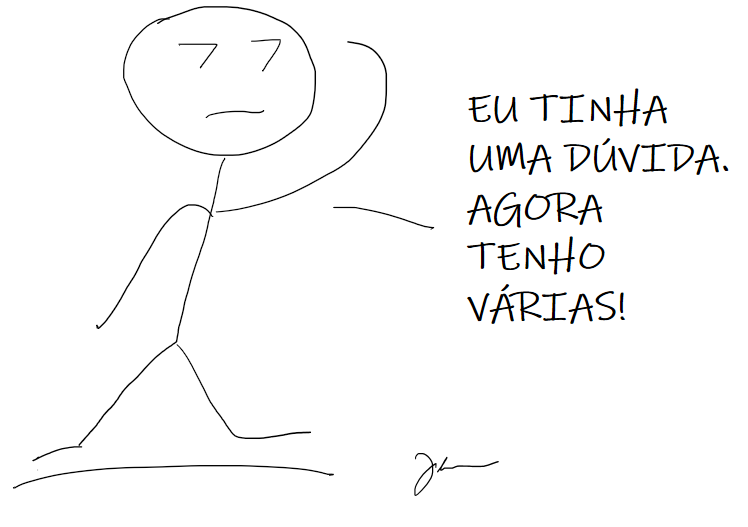
\includegraphics[width=0.5\linewidth]{../Imagens/ebook_duvida_01} 

}

\caption{Tenho uma dúvida}\label{fig:fig01}
\end{figure}

Calma meu jovem. Vamos ver outras definições então!

\begin{quote}
A Estatística é a ciência que fornece métodos para a coleta, organização, descrição ou apresentação, análise e interpretação de dados para suportar a tomada de decisão. --- Adaptação
\end{quote}

O dicionário do Google também define como:

\begin{quote}
Ramo da matemática que trata da coleta, da análise, da interpretação e da apresentação de massas de dados numéricos. --- Google
\end{quote}

Temos mais algumas frases a seguir!

\begin{quote}
A estatística é a arte de nunca ter que dizer que você está errado. --- C. J. Bradfield
\end{quote}

Ou ainda minha favorita!

\begin{quote}
Estatística é a arte de torturar os números até que eles confessem. --- Desconhecido
\end{quote}

\begin{figure}[H]

{\centering 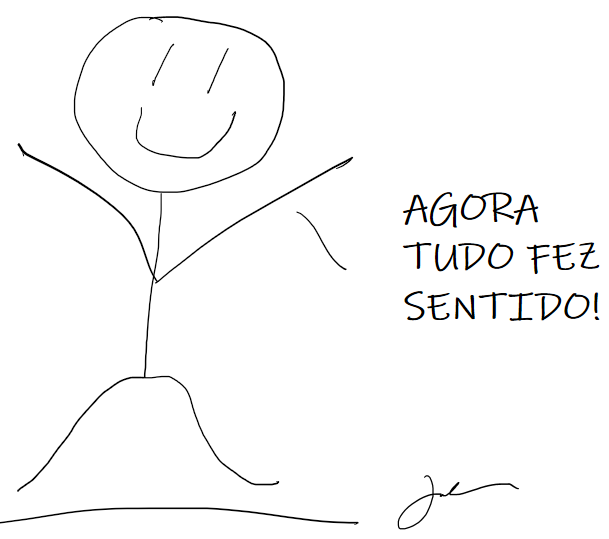
\includegraphics[width=0.5\linewidth]{../Imagens/ebook_duvida_02} 

}

\caption{Não tenho mais dúvidas}\label{fig:fig02}
\end{figure}

Nos dias atuais, cada vez mais as pessoas, empresas e governos estão tomando decisões com base em dado e como podemos ver das definições acima, a ciência estatística possui relação direta com a descoberta de conhecimento através de dados. Isso faz com que esta ciência seja de total relevância para quem quer descobrir e entender o que seus dados estão tentando esconder.

O processo de coleta, organização, descrição dos dados, cálculo e interpretação de estatísticas pertencem à \textbf{Estatística descritiva}, enquanto a análise e a interpretação dos dados, associado a uma margem de incerteza, geralmente associada a uma \textbf{amostra} ficam por conta da \textbf{Estatística inferencial ou indutiva} fortemente fundamentada na teoria das probabilidades que veremos em módulo específico.

\hypertarget{fases-do-trabalho-estatistico}{%
\section{Fases do trabalho estatístico}\label{fases-do-trabalho-estatistico}}

\begin{itemize}
\tightlist
\item
  \textbf{Definição do problema}: A figura \ref{fig:fig00} exibe um \emph{roadmap} do processo estatístico. Este processo inicia sempre pela \textbf{Definição do problema}. Nesta fase inicial é preciso delimitar muito bem o problema de pesquisa. Seja ele simples ou complexo, se esta etapa for mal pensada, poderá conduzir a resultados inesperados ou questões não respondidas;
\end{itemize}

\begin{figure}[H]

{\centering 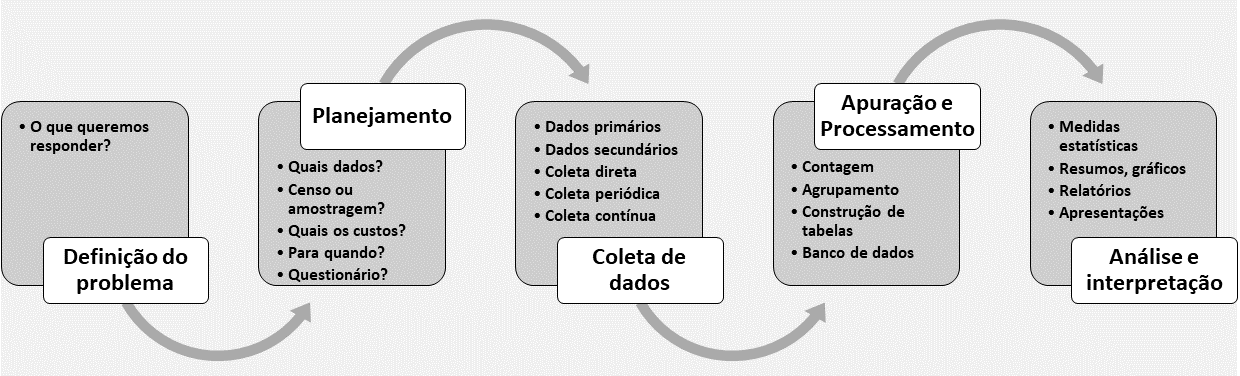
\includegraphics[width=1\linewidth]{../Imagens/ebook_processo_estats} 

}

\caption{Fases do trabalho estatístico}\label{fig:fig00}
\end{figure}

\begin{itemize}
\item
  \textbf{Planejamento: } Nesta etapa é preciso responder muitos porquês, afinal não podem restar dúvidas que comprometam futuramente os trabalhos. Deve-se responder questões sobre quais dados utilizar, tamanho e tipo das amostras, custos do projeto, tempo de execução, ferramentas, pessoal qualificado e uma série de questões relacionadas ao projeto.
\item
  \textbf{Coleta dos dados: } Na etapa de coleta, o pesquisador deve estar atento ás fontes de dados e à qualidade dos mesmos. Seja através de questionários ou de bases já montadas, os dados precisam ser confiáveis e consistentes. Os dados devem ser catalogados respeitando-se o tipo de coleta, se periódica, se contínua, se os dados são primários (gerados pela própria empresa ou pesquisador) ou secundários (gerados por terceiros).
\item
  \textbf{Apuração: } Esta etapa serve para qualificar os dados e nela são feitas contagens, tabulações, agrupamentos e inserção em bancos de dados para o trabalho de análise.
\item
  \textbf{Análise e interpretação: } Nesta fase todo o ferramental estatístico entra em ação para analisar e descobrir as relações entre as variáveis buscando responder às hipóteses do problema de pesquisa. A geração de relatórios, apresentações e painéis (\emph{dashboards}) fazem parte desta etapa e auxiliarão na tomada de decisão e na geração de conhecimento.
\end{itemize}

\hypertarget{como-utilizar-estatistica}{%
\section{Como utilizar estatística?}\label{como-utilizar-estatistica}}

Esta é uma pergunta vastas, mas com base em nossa experiência e na comunidade estatística, segue nove boas práticas para direcionar o pesquisador.

\begin{itemize}
\item
  \textbf{Estatística deve ser utilizada para ajudar a responder perguntas científicas:} É importante inserir estatística desde o planejamento do experimento até a condução das análises e por fim a compilação dos conhecimentos adquiridos com base nos dados gerados pela pesquisa.
\item
  \textbf{Pessoas se enganam. Dados não:} Isso é verdade, mas tome cuidado, pois sinais sempre vêm com ruído. Por isso é fundamental entender muito bem o problema de pesquisa e conhecer seus dados para saber diferenciar dado bom de ruído. Questione as fontes e as formas que te foram apresentadas.
\item
  \textbf{Planejamento com foco no presente e no futuro:} Este é um dos princípios mais violados nas ciências, portanto fique alerta. Fazer as perguntas certas e obter as respostas adequadas pode evitar perda de tempo, dinheiro e dores de cabeça na hora de analisar os dados obtidos de experimento mal delineado.
\item
  \textbf{Atenção à qualidade dos dados:} Se você tiver acesso ao processo de planejamento e coleta de dados seja cuidadoso e tenha em mente os impactos futuros na condução das análises. Dados ruim pode arruinar um estudo ou conduzir a resultados errados.
\end{itemize}

\begin{figure}[H]

{\centering 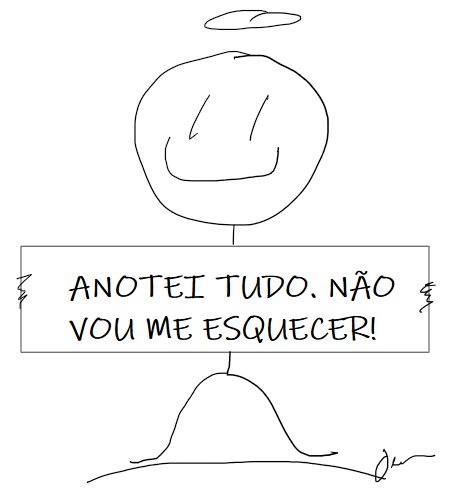
\includegraphics[width=0.5\linewidth]{../Imagens/ebook_anima_03} 

}

\caption{Anotei tudo}\label{fig:fig03}
\end{figure}

\begin{itemize}
\item
  \textbf{Estatística não é só técnica:} Análise estatística é mais que um software. O software estatístico fornece ferramentas para auxiliar a análise, não para defini-las. O contexto científico é crítico, e a chave para a análise estatística baseada em princípios é aproximar os métodos analíticos das questões científicas e de negócio.
\item
  \textbf{Busque a simplicidade:} As pessoas não gostam de complexidade. Uma boa parte dos modelos estatísticos exige formulação simples. Em muitos casos, uma simples análise descritiva resolve o problema. Tenha em mente que um grande número de medições, dados ausentes, erros, vieses de amostragem e outros fatores podem aumentar a complexidade do modelo e tornar o estudo impraticável.
\item
  \textbf{Calcule a variabilidade:} faz parte da análise estatística justamente ajudar a avaliar a incerteza, muitas vezes na forma de um erro padrão ou intervalo de confiança, e um dos grandes sucessos da modelagem estatística e inferência é que ela pode fornecer estimativas de erros padrão dos mesmos dados. Ao apresentar resultados, é essencial fornecer alguma noção de incerteza estatística envolvida em seu estudo.
\item
  \textbf{Verifique as suposições das suas técnicas:} É importante entender as suposições por trás dos métodos estatísticos e fazer o que for possível para entender e avaliar essas suposições. Não deixe que o software faça o papel do analista, ele apenas deve auxiliá-lo no processamento dos dados e nos cálculos. A validação das técnicas e as interpretações são sempre por conta do analista.
\item
  \textbf{Torne seu trabalho reprodutível:} Resultados replicáveis são fundamentais para que outros pesquisadores/analistas possam revisitar e reprocessar seus achados. Em muitos contextos, a replicação completa é muito difícil ou impossível, como em experimentos de larga escala, como ensaios clínicos multicêntricos, porém é sempre bom perseguir esta meta. Quando possível, forneça o conjunto de dados, juntamente com uma descrição completa da análise. Com isso deve ser possível reproduzir as tabelas, figuras e inferências estatísticas. Melhore drasticamente a capacidade de reproduzir descobertas sendo muito sistemático sobre as etapas da análise, compartilhando os dados e o código usados para produzir os resultados e seguindo as práticas recomendadas de estatística aceitas.
\end{itemize}

\hypertarget{como-nao-utilizar-estatistica}{%
\section{Como não utilizar estatística?}\label{como-nao-utilizar-estatistica}}

Aqui listamos também nove pontos de atenção para evitar mal uso da estatística.

\begin{itemize}
\item
  \textbf{Não minta com estatística:} Alguns pesquisadores podem ser tentados a maquiar algum dados para seu benefício ou de outros. É sempre bom ter em mente que sua reputação e carreira podem estar em jogo ao apresentar falsos resultados. Sugerimos aqui uma leitura extra do livro do \href{https://www.amazon.com.br/Como-Mentir-Estat\%C3\%ADstica-Darrell-Huff/dp/858057952X}{Darrell Huff}, pois para não mentir é importante saber como se mente com estatística.
\item
  \textbf{Resista aos mau intencionados:} Se alguém te pediu pra fazer algo estatisticamente ilegal ou aplicar uma técnica inadequada, seja resistente e questione. Nem sempre o problema é simples, então é sempre bom ter uma compreensão da situação como um todo. Aprenda a dizer não para evitar problemas futuros.
\end{itemize}

\begin{figure}[H]

{\centering 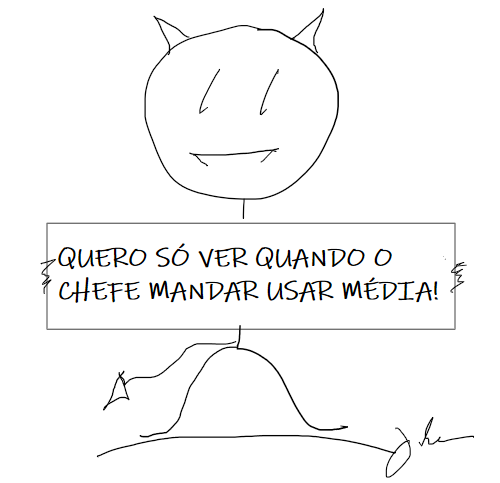
\includegraphics[width=0.5\linewidth]{../Imagens/ebook_anima_04} 

}

\caption{Use a média}\label{fig:fig04}
\end{figure}

\begin{itemize}
\item
  \textbf{Cuidado com as suposições:} É melhor assumir que não tem a resposta no momento e que a traz em outro momento do que inventar suposições incorretas só pra não sair por baixo em uma conversa. Ou pior, realizar um estudo/projeto apoiado por suposições incorretas sobre uma técnica estatística. Cedo ou tarde e você poderá se por em uma saia justa e ter de voltar atrás.
\item
  \textbf{Evite ambiguidades:} A comunicação estatística precisa ser clara. Em termos estatísticos não há espaço para meias verdades, pois são os dados falando.
\item
  \textbf{Tenha certeza do que está falando:} Não subestime seu público. É verdade que algumas pessoas não falam ou entendem bem o \emph{estatiquês}, mas fique alerta, pois muitos são conhecedores desta ciência, então por vias das dúvidas é melhor saber o que você vai comunicar para evitar constrangimentos.
\item
  \textbf{Não seja complexo demais nas suas análises e comunicações:} Neste ponto seja ponderado, pois nem tudo que é simples é fácil e nem tudo que é difícil é complexo. Do planejamento à entrega é sempre bom ter seu trabalho revisado / acompanhado por outra pessoa de forma a identificar pontos de melhoria. A linguagem, sempre que possível deve ser de simples compreensão.
\item
  \textbf{Maria vai com as outras:} Muito cuidado. Não é porque todo mundo faz algo de um jeito que você pode assumir que é certo. Censo crítico faz toda a diferença na identificação deste tipo de fenômeno.
\item
  \textbf{Cuidado como modelos automáticos:} Modelos automatizados ou semi-automatizados podem às vezes gerar saídas inesperadas. \emph{``.. todos os modelos são errados, mas alguns são úteis. --- George E. P. Box''}. Com a popularização do \emph{machine learning}
  muitas pessoas tendem a pensar que se colocar os dados no computador e passar o algoritmo tudo ficará pronto. Temos casos recentes de que isso é possível. Não vamos entrar no mérito, mas como já comentamos antes, a inteligência é do analista e saídas imprevistas podem ocorrer.
\item
  \textbf{Não acredite apenas na estatística:} Pois é. A estatística é fundamental e sem ela nada podemos fazer com os dados, mas esteja sempre atento ao negócio ou qualquer evento externo que possa influenciar seus resultados.
\end{itemize}

\hypertarget{estatistica-data-science-e-big-data.}{%
\section{\texorpdfstring{Estatística, \emph{Data Science} e \emph{Big Data}.}{Estatística, Data Science e Big Data.}}\label{estatistica-data-science-e-big-data.}}

Desde que o conceito de dado passou a existir, a estatística se faz presente. A seguir um pequeno texto que relaciona a estatística com \emph{Data Science} e \emph{Big Data}.

Estatística e \emph{Data Science} (Ciência de Dados) são partes inseparáveis. De certa forma, a estatística é um subconjunto da ciência de dados. Mas o que é \emph{Data Science}? É difícil definir um conceito tão amplo porém, a \emph{Wikipedia} Norte Americana coloca da seguinte forma:

\begin{quote}
\emph{Data science, also known as data-driven science, is an interdisciplinary field about scientific methods, processes and systems to extract knowledge or insights from data in various forms, either structured or unstructured, similar to Knowledge Discovery in Databases (KDD)}. Fonte: \url{https://www.wikiwand.com/en/Data_science}, acesso em ``28/02/2019''
\end{quote}

No texto acima podemos isolar o termo \emph{interdisciplinary} que remete a um conjunto de muitas áreas do conhecimento. Podemos marcar desta definição aos conceitos:

\begin{itemize}
\tightlist
\item
  \textbf{Métodos Científicos} - Métodos estatísticos e computacionais, por exemplo;
\item
  \textbf{Processos} - Organização de passos para atingir um objetivo;
\item
  \textbf{Sistemas} - Sistemas informatizados, por exemplo, são ferramentas superpoderosas para realizar \emph{Data Science}.
\end{itemize}

Tudo com objetivo de obter conhecimento com base em dados, sejam eles estruturados ou não estruturados. Expandindo mais um pouco, pode-se incluir o termo \emph{Big Data} que envolve dados estruturados ou não estruturados em grandes volumes. O conceito de \emph{Big Data} também é complexo e discutível. \citep{de2016formal} propõem uma definição deste termo como segue.

\begin{quote}
\emph{Big Data is the Information asset characterized by such a High Volume, Velocity and Variety to require specific Technology and Analytical Methods for its transformation into Value.}
\end{quote}

Deixamos ao leitor interessado consultar \citep{de2016formal} para mais definições sobre \emph{Big Data}.

Podemos isolar nesta definição os termos:

\begin{itemize}
\tightlist
\item
  \textbf{Volume Alto} - O termos alto pode ser relativo e depende do tipo de computador que está suportando a análise. Nós entendemos como volume alto qualquer base de dados que não pode ser processada por um sistema de tabulação como \emph{LibreOffice calc} e seu concorrente da \emph{Microsoft};
\item
  \textbf{Velocidade} - Grandes bases exigem processamento rápido e algorítimos rápidos muitas vezes são mais relevantes que um bom \emph{Hardware};
\item
  \textbf{Variedade} - Bancos de dados de fontes diversas podem ser relacionados para obter conhecimento.
\end{itemize}

Estes termos chave estão direcionados diretamente com tecnologia e métodos estatísticos para transformar dados o obter valor ou seja, conhecimento. Aqui percebemos que \emph{Data Science}, \emph{Big Data} possuem muito em comum. Ambas utilizam dados como combustível visando descobrir novos conhecimentos. Ou seja, tudo isso precisa de estatística para fazer sentido.

Com base nos conceitos até aqui, poderíamos sugerir nossa própria definição de \emph{Data Science}.

\begin{quote}
``Data Science é uma ciência ampla que une métodos científicos como a estatística, processos e sistemas tecnológicos buscando, através da análise de dados, sejam eles simples ou \emph{Big Data} estruturados ou não, obter conhecimento acerca de fenômenos e processos variados''.
\end{quote}

\hypertarget{conceitos-e-definicoes}{%
\section{Conceitos e definições}\label{conceitos-e-definicoes}}

A partir de agora iniciamos os estudos de estatística. Para começar vamos revisar alguns dos conceitos utilizados na linguagem estatística de forma simplificada.

\begin{Shaded}
\begin{Highlighting}[]
\CommentTok{# Carregando funções extras do rnp}
\KeywordTok{require}\NormalTok{(rnp, }\DataTypeTok{quietly =} \OtherTok{TRUE}\NormalTok{)}

\CommentTok{# Classes para base de dados das IES}
\NormalTok{dicionario <-}\StringTok{ "Dados/INEP/ANEXOS/ANEXO I - Dicionаrio de Dados e Tabelas Auxiliares/Dicionаrio_de_Dados.xlsx"}
\NormalTok{classes <-}\StringTok{ }\NormalTok{rnp}\OperatorTok{::}\KeywordTok{rnp_get_classes_inep}\NormalTok{(}\DataTypeTok{caminho =}\NormalTok{ dicionario, }
                                     \DataTypeTok{aba =} \StringTok{"DM_IES"}\NormalTok{, }
                                     \DataTypeTok{retorna_lista =} \OtherTok{FALSE}\NormalTok{)}

\CommentTok{# Base de dados  }
\NormalTok{base <-}\StringTok{ }\NormalTok{rnp}\OperatorTok{::}\KeywordTok{rnp_read}\NormalTok{(}\DataTypeTok{base =} \KeywordTok{paste0}\NormalTok{(}\StringTok{"Dados/INEP/DADOS/DM_IES.CSV"}\NormalTok{),}
                      \DataTypeTok{sep =} \StringTok{"|"}\NormalTok{, }
                      \DataTypeTok{dec =} \StringTok{"."}\NormalTok{, }
                      \DataTypeTok{header =} \OtherTok{TRUE}\NormalTok{, }
                      \DataTypeTok{encoding =} \StringTok{"Latin-1"}\NormalTok{,}
                      \DataTypeTok{verbose =} \OtherTok{FALSE}\NormalTok{, }
                      \DataTypeTok{showProgress =} \OtherTok{FALSE}\NormalTok{)}
\CommentTok{# Aplica classes}
\NormalTok{base_ies <-}\StringTok{ }\NormalTok{rnp}\OperatorTok{::}\KeywordTok{rnp_aplica_classes}\NormalTok{(}\DataTypeTok{base =}\NormalTok{ base, }\DataTypeTok{classes =}\NormalTok{ classes) }\OperatorTok\StringTok{ }
\StringTok{    }\NormalTok{dplyr}\OperatorTok{::}\KeywordTok{mutate}\NormalTok{(}\DataTypeTok{Sigla =}\NormalTok{ SG_IES,}
                  \DataTypeTok{TotalTecnicos =}\NormalTok{ QT_TEC_TOTAL, }
                  \DataTypeTok{ReceitaPropria =}\NormalTok{ VL_RECEITA_PROPRIA,}
                  \DataTypeTok{DespesaPesquisa =}\NormalTok{ VL_DESPESA_PESQUISA)}

\NormalTok{base_ies }\OperatorTok\StringTok{ }
\StringTok{  }\NormalTok{dplyr}\OperatorTok{::}\KeywordTok{select}\NormalTok{(Sigla, TotalTecnicos, ReceitaPropria,DespesaPesquisa) }\OperatorTok\StringTok{ }
\StringTok{  }\KeywordTok{head}\NormalTok{(}\DataTypeTok{n =} \DecValTok{10}\NormalTok{) }\OperatorTok\StringTok{ }
\StringTok{  }\NormalTok{knitr}\OperatorTok{::}\KeywordTok{kable}\NormalTok{(}\DataTypeTok{digits =} \DecValTok{2}\NormalTok{, }\DataTypeTok{align =} \StringTok{"llrrr"}\NormalTok{, }
             \DataTypeTok{booktabs =} \OtherTok{TRUE}\NormalTok{, }\DataTypeTok{format =}\NormalTok{ tb_formata,}
             \DataTypeTok{caption =} \StringTok{"Dez primeiras observações da base de IES censo 2017"}\NormalTok{) }\OperatorTok\StringTok{ }
\StringTok{  }\NormalTok{kableExtra}\OperatorTok{::}\KeywordTok{kable_styling}\NormalTok{(}\DataTypeTok{latex_options =} \StringTok{"hold_position"}\NormalTok{)}
\end{Highlighting}
\end{Shaded}

\begin{table}[!h]

\caption{\label{tab:tab01}Dez primeiras observações da base de IES censo 2017}
\centering
\begin{tabular}{llrrrllrrrllrrrllrrr}
\toprule
Sigla & TotalTecnicos & ReceitaPropria & DespesaPesquisa\\
\midrule
UFMT & 1574 & 6913132 & 5807924\\
UNB & 3206 & 63239902 & 5772538\\
UFS & 1429 & 3161937 & 3033336\\
UFAM & 1721 & 4136205 & 1490991\\
UFOP & 786 & 3458763 & 748715\\
\addlinespace
PUCPR & 1275 & 616991005 & 11948066\\
UNICAP & 441 & 142785305 & 560400\\
UCS & 986 & 338035351 & 3380182\\
UNISINOS & 1062 & 487902230 & 6687713\\
UCPEL & 246 & 100089191 & 3540465\\
\bottomrule
\end{tabular}
\end{table}

\hypertarget{populacao-amostra-censo}{%
\subsection{População, amostra, censo}\label{populacao-amostra-censo}}

\begin{itemize}
\item
  \textbf{População:} É o conjunto de todos os elementos (pessoas, animais, plantas, etc.) que possuam alguma característica de interesse.
\item
  \textbf{Amostra:} É um pedaço ou subconjunto da população e, a partir dela, faz-se inferência sobre as características da população. A ideia de amostra significativa vem do fato de que para representar a população, a amostra precisa preservar suas características.
\end{itemize}

\begin{figure}[H]

{\centering 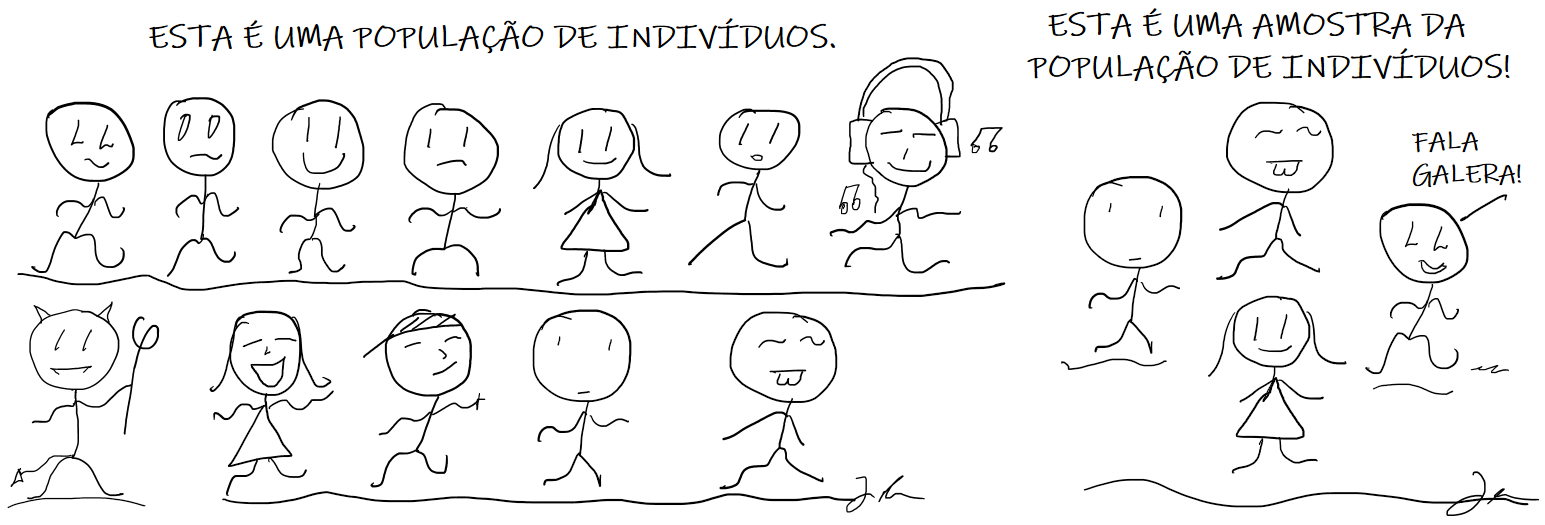
\includegraphics[width=1\linewidth]{../Imagens/ebook_anima_05} 

}

\caption{População e amostra}\label{fig:fig05}
\end{figure}

\begin{itemize}
\item
  \textbf{Censo:} É o processo utilizado para coletar dados abordando todos os elementos de uma população. Neste caso não há necessidade de amostras, pois toda a população é considerada.
\item
  \textbf{Parâmetro: } É qualquer medida numérica que serve para descrever uma \textbf{característica de uma população}. São geralmente representados por letras gregas. Por exemplo: média (\(\mu\)), variância (\(\sigma^2\)) e desvio padrão (\(\sigma\)).
\item
  \textbf{Estatística: } Tem a mesma função do parâmetro, porém é medido na amostra. São geralmente representados por letras latinas com acentos. Por exemplo: média amostral (\(\bar X\)), variância (\(S^2\)) e desvio padrão (\(S\)) amostrais.
\end{itemize}

\hypertarget{dados-informacao-e-conhecimento}{%
\subsection{Dados, informação e conhecimento}\label{dados-informacao-e-conhecimento}}

\begin{itemize}
\item
  \textbf{Dados: }Dados são resultados de medições ou qualquer fonte relato documentado. Por si só dados não tem significado concreto porém, a disponibilidade dos mesmos é matéria prima para a obtenção de informações. Dados podem ser obtidos pela percepção através dos sentidos, pela execução de um processo de medição, por sensores, pesquisas, censos, etc.
\item
  \textbf{Informação:} O processamento e análise dos dados gera informação que auxilia a tomada de decisão seja nos negócios, pela ciência e na vida cotidiana em geral.
\item
  \textbf{Conhecimento:} O conhecimento extrapola a informação, ele produz ideias e experiências. Através do conhecimento é possível a abstração e a evolução de ideias e conceitos novos com base em todo tipo de experiência, sejam elas oriundas das informações ou vivências.
\end{itemize}

\hypertarget{variaveis}{%
\subsection{Variáveis}\label{variaveis}}

Variáveis são características medidas em cada elemento da amostra ou população. Elas podem ter valores numéricos ou não numéricos e seus valores podem varia de elemento para elemento.

\begin{figure}[H]

{\centering 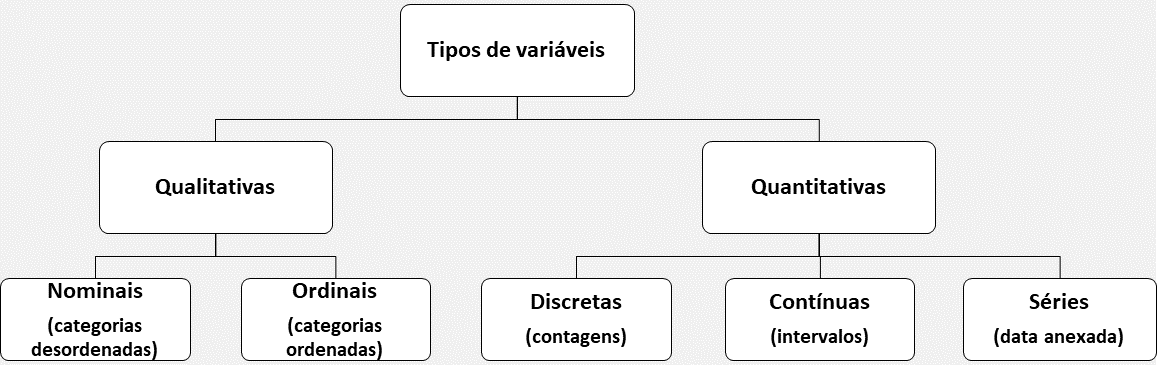
\includegraphics[width=1\linewidth]{../Imagens/ebook_variaveis2} 

}

\caption{Tipos de variáveis}\label{fig:fig06}
\end{figure}

A figura \ref{fig:fig06} trás um resumo dos tipos mais comuns de variáveis. Detalhamos um pouco mais a seguir.

\begin{itemize}
\item
  \textbf{Variáveis numéricas:} As variáveis numéricas ou quantitativas se classificam em discretas e contínuas. As discretas persentam contagens e as contínuas, medidas. Na tabela \ref{tab:tab01}, a coluna \texttt{TotalTecnicos} que representa o total de técnicos das IES é um bom exemplo de variável quantitativa discreta. Já as colunas \texttt{ReceitaPropria\ \ e\ DespesaPesquisa} são variáveis contínuas, pois são medidas que representam valores de receita.
\item
  \textbf{Séries temporais:} As variáveis quantitativas quando indexadas de uma variável de tempo, como por exemplo hora, dia, mês, ano, etc. são classificadas como séries temporais. Séries temporais possuem um grande valor e por isso, a estatística reserva um campo completo de estudos para este tipo de dado.
\item
  \textbf{Variáveis categóricas:} As variáveis categóricas ou qualitativas descrevem caraterísticas dos indivíduos da amostra ou população. Elas podem ser nominais, quando descrevem características arbitrárias sem efeito de ordenação ou ordinais, quando descrevem relações de ordenação. A coluna \texttt{Sigla} da tabela \ref{tab:tab01} representa uma variável qualitativa nominal. Exemplos de ordinais são \texttt{classe\ social} e \texttt{escolaridade}
\end{itemize}

\hypertarget{analise-univariada-bivariada-e-multivariada}{%
\subsection{Análise univariada, bivariada e multivariada}\label{analise-univariada-bivariada-e-multivariada}}

\begin{itemize}
\item
  \textbf{A análise univariada:} Busca-se descrever a população ou amostra analisando cada variável de forma isolada. É a maneira mais simples de obter informação e de fazer a estimativa estatística. Exemplos de análises univariadas são as médias, medianas e quatis.
\item
  \textbf{A análise bivariada:} Analisa relações existentes entre pares de variáveis para fins de explicação e/ou previsão. Na análise bivariada, a formulação de uma hipótese precisar ser feita e a estatística permitirá inferir ou confirmar esta hipótese. Análise de correção entre duas variáveis e tabelas de frequência de dupla entrada são exemplos de análise bivariada
\item
  \textbf{A análise multivariada:} Na análise multivariada a estatística dispões de uma série de técnicas que analisam de forma conjunta as múltiplas relações das variáveis. Regressão múltipla, análise de cluster e fatorial são exemplos de análises multivariadas.
\end{itemize}

\hypertarget{tidydata}{%
\subsection{\texorpdfstring{\emph{tidydata}}{tidydata}}\label{tidydata}}

Em seu artigo, \citep{wickham2014tidy} discutem e mostram uma forma repensada de organizar tabelas estruturadas para análise de dados. De forma simples, um significado para \emph{\texttt{tidy\ data}} é: dados arrumados, organizados.
Um conjunto de dados para ser \texttt{tidy} precisa ter três ingredientes:

\begin{itemize}
\tightlist
\item
  Cada observação é uma linha;
\item
  Cada variável é uma coluna;\\
\item
  Cada valor está em uma célula (linha x coluna);
\end{itemize}

Dados neste formato ajudam a tornar a análise mais rápida, principalmente com as ferramentas do \texttt{tidyverso} \citep{wickham2017tidyverse}. A Tabela \ref{tab:tab01} mostra uma configuração de dados \texttt{tidy}, onde cada linha representa uma observação ou indivíduo que no caso é uma IES; cada coluna representa uma variável ou característica, por exemplo \texttt{Sigla} ou \texttt{ReceitaPropria} da IES e o cruzamento entre linhas e colunas são os valores correspondentes.

\textbf{Observação:} Nas empresas o conceito de \texttt{tidy\ data} geralmente é atribuído ao que chamam de \texttt{ABT\ (Analytics\ Base\ Table)}. Este é o estado da arte que nem sempre é fácil de se chagar, mas uma vez lá, os dados estarão prontos para todo tipo de análise de modelagem.

\begin{Shaded}
\begin{Highlighting}[]
\CommentTok{# Exemplos de tidydasets}
\NormalTok{knitr}\OperatorTok{::}\KeywordTok{kable}\NormalTok{(}
  \KeywordTok{list}\NormalTok{(}\KeywordTok{head}\NormalTok{(mtcars[,}\DecValTok{1}\OperatorTok{:}\DecValTok{4}\NormalTok{], }\DecValTok{10}\NormalTok{), }\KeywordTok{head}\NormalTok{(dplyr}\OperatorTok{::}\NormalTok{starwars[,}\DecValTok{1}\OperatorTok{:}\DecValTok{4}\NormalTok{], }\DecValTok{10}\NormalTok{)),}
  \DataTypeTok{booktabs =} \OtherTok{TRUE}\NormalTok{, }\DataTypeTok{format =}\NormalTok{ tb_formata, }
  \DataTypeTok{caption =} \StringTok{"Amostra de outras tabelas de dados organizados"}\NormalTok{) }\OperatorTok\StringTok{ }
\StringTok{  }\NormalTok{kableExtra}\OperatorTok{::}\KeywordTok{kable_styling}\NormalTok{(}\DataTypeTok{latex_options =} \StringTok{"hold_position"}\NormalTok{)}
\end{Highlighting}
\end{Shaded}

\begin{table}[!h]
\caption{\label{tab:tab02}Amostra de outras tabelas de dados organizados}

\centering
\begin{tabular}{lrrrr}
\toprule
  & mpg & cyl & disp & hp\\
\midrule
Mazda RX4 & 21.0 & 6 & 160.0 & 110\\
Mazda RX4 Wag & 21.0 & 6 & 160.0 & 110\\
Datsun 710 & 22.8 & 4 & 108.0 & 93\\
Hornet 4 Drive & 21.4 & 6 & 258.0 & 110\\
Hornet Sportabout & 18.7 & 8 & 360.0 & 175\\
\addlinespace
Valiant & 18.1 & 6 & 225.0 & 105\\
Duster 360 & 14.3 & 8 & 360.0 & 245\\
Merc 240D & 24.4 & 4 & 146.7 & 62\\
Merc 230 & 22.8 & 4 & 140.8 & 95\\
Merc 280 & 19.2 & 6 & 167.6 & 123\\
\bottomrule
\end{tabular}
\centering
\begin{tabular}{lrrl}
\toprule
name & height & mass & hair\_color\\
\midrule
Luke Skywalker & 172 & 77 & blond\\
C-3PO & 167 & 75 & NA\\
R2-D2 & 96 & 32 & NA\\
Darth Vader & 202 & 136 & none\\
Leia Organa & 150 & 49 & brown\\
\addlinespace
Owen Lars & 178 & 120 & brown, grey\\
Beru Whitesun lars & 165 & 75 & brown\\
R5-D4 & 97 & 32 & NA\\
Biggs Darklighter & 183 & 84 & black\\
Obi-Wan Kenobi & 182 & 77 & auburn, white\\
\bottomrule
\end{tabular}
\end{table}

\pagebreak

\begin{center}\rule{0.5\linewidth}{\linethickness}\end{center}

\begin{Shaded}
\begin{Highlighting}[]
\NormalTok{.}
\end{Highlighting}
\end{Shaded}

\hypertarget{exercicios-resolvidos}{%
\subsection{Exercícios resolvidos}\label{exercicios-resolvidos}}

Com apoio da base de IES, cuja amostra foi mostrada na tabela \ref{tab:tab01} vamos exercitar os conceitos vistos até agora.

\begin{itemize}
\tightlist
\item
  \textbf{População e amostra}
\end{itemize}

\BeginKnitrBlock{exercise}
\protect\hypertarget{exr:unnamed-chunk-6}{}{\label{exr:unnamed-chunk-6} }Quem é a população de IES?
\EndKnitrBlock{exercise}

\BeginKnitrBlock{solution}
\iffalse{} {Solução. } \fi{}Neste caso, a população se confunde com um censo, pois a base das IES faz parte do levantamento censitário de 2017 e contempla, a princípio todas as IES do Brasil
\EndKnitrBlock{solution}

\begin{Shaded}
\begin{Highlighting}[]
\KeywordTok{paste}\NormalTok{(}\KeywordTok{nrow}\NormalTok{(base_ies), }\StringTok{"Universidades."}\NormalTok{)}
\end{Highlighting}
\end{Shaded}

\begin{verbatim}
## [1] "2448 Universidades."
\end{verbatim}

\BeginKnitrBlock{exercise}
\protect\hypertarget{exr:unnamed-chunk-9}{}{\label{exr:unnamed-chunk-9} }O que poderia ser uma amostra da base de IES?
\EndKnitrBlock{exercise}

\BeginKnitrBlock{solution}
\iffalse{} {Solução. } \fi{}Uma amostra poderia ser todas as IES grandes com mais de 2000 técnicos.
\EndKnitrBlock{solution}

\begin{Shaded}
\begin{Highlighting}[]
\KeywordTok{paste}\NormalTok{(}\StringTok{"A base tem"}\NormalTok{, base_ies }\OperatorTok\StringTok{ }\KeywordTok{filter}\NormalTok{(TotalTecnicos }\OperatorTok{>}\StringTok{ }\DecValTok{2000}\NormalTok{) }\OperatorTok\StringTok{ }\KeywordTok{nrow}\NormalTok{(), }\StringTok{"IES com mais de 2000 ténicos"}\NormalTok{)}
\end{Highlighting}
\end{Shaded}

\begin{verbatim}
## [1] "A base tem 29 IES com mais de 2000 ténicos"
\end{verbatim}

\BeginKnitrBlock{exercise}
\protect\hypertarget{exr:unnamed-chunk-12}{}{\label{exr:unnamed-chunk-12} }Defina um parâmetro desta base.
\EndKnitrBlock{exercise}

\BeginKnitrBlock{solution}
\iffalse{} {Solução. } \fi{}Neste caso poderíamos definir \(\mu_{receita}\) como a receita própria média das IES brasileiras.
\EndKnitrBlock{solution}

\BeginKnitrBlock{exercise}
\protect\hypertarget{exr:unnamed-chunk-14}{}{\label{exr:unnamed-chunk-14} }Qual seria uma estatística?
\EndKnitrBlock{exercise}

\BeginKnitrBlock{solution}
\iffalse{} {Solução. } \fi{}A receita média média da amostra de SP pode ser definida uma estatística dada por \(\bar X_{receita}\)
\EndKnitrBlock{solution}

\begin{itemize}
\tightlist
\item
  \textbf{Dados, informação e conhecimento}
\end{itemize}

\BeginKnitrBlock{exercise}
\protect\hypertarget{exr:unnamed-chunk-16}{}{\label{exr:unnamed-chunk-16} }A tabela de IES possui muitos registros numéricos e também textuais. Ela representa melhor, dados, informações ou conhecimento?
\EndKnitrBlock{exercise}

\BeginKnitrBlock{solution}
\iffalse{} {Solução. } \fi{}Valores brutos em uma tabela são exemplos de dados que por sí só não são informação. Assim a tabela representa um conjunto de \textbf{dados}
\EndKnitrBlock{solution}

\BeginKnitrBlock{exercise}
\protect\hypertarget{exr:unnamed-chunk-18}{}{\label{exr:unnamed-chunk-18} }A frase, `O estado de São Paulo possui o maior número de IES do Brasil' é um exemplo de dado, informação ou conhecimento?
\EndKnitrBlock{exercise}

\BeginKnitrBlock{solution}
\iffalse{} {Solução. } \fi{}Estas informações podem ser obtidas dos conjuntos de dados das IES através de uma contagem de toda as IES do estado de São Paulo
\EndKnitrBlock{solution}

\BeginKnitrBlock{exercise}
\protect\hypertarget{exr:unnamed-chunk-20}{}{\label{exr:unnamed-chunk-20} }``Um estado que possui muitas universidade possui indicadores de educação superiores.'' Esta frase é um exemplos de\ldots{}
\EndKnitrBlock{exercise}

\BeginKnitrBlock{solution}
\iffalse{} {Solução. } \fi{}Conhecimento abstraído do fato de que muitas universidades em um estado podem representar alto índice de formação de seu povo.
\EndKnitrBlock{solution}

\begin{itemize}
\tightlist
\item
  \textbf{Variáveis e tipos de análises}
\end{itemize}

\BeginKnitrBlock{exercise}
\protect\hypertarget{exr:unnamed-chunk-22}{}{\label{exr:unnamed-chunk-22} }No conjunto de IES temos quantas variáveis e quantas observações?
\EndKnitrBlock{exercise}

\BeginKnitrBlock{solution}
\iffalse{} {Solução. } \fi{}A base IES possui 2448 linhas (observações) e 4 colunas (variáveis). Além disso, são uma variável caractere e três numéricas conforme resultados abaixo, obtidos com a função extra \texttt{rnp\_atributos()}.
\EndKnitrBlock{solution}

\begin{Shaded}
\begin{Highlighting}[]
\CommentTok{# Listando os atributos da base de ies para as 10 primeiras colunas}
\NormalTok{rnp}\OperatorTok{::}\KeywordTok{rnp_atributos}\NormalTok{(base_ies) }\OperatorTok\StringTok{ }
\StringTok{  }\KeywordTok{head}\NormalTok{(}\DataTypeTok{n =} \DecValTok{10}\NormalTok{) }\OperatorTok\StringTok{ }
\StringTok{  }\NormalTok{knitr}\OperatorTok{::}\KeywordTok{kable}\NormalTok{(}\DataTypeTok{booktabs =} \OtherTok{TRUE}\NormalTok{, }\DataTypeTok{format =}\NormalTok{ tb_formata) }\OperatorTok\StringTok{ }
\StringTok{  }\NormalTok{kableExtra}\OperatorTok{::}\KeywordTok{kable_styling}\NormalTok{(}\DataTypeTok{latex_options =} \StringTok{"hold_position"}\NormalTok{)}
\end{Highlighting}
\end{Shaded}

\begin{table}[!h]
\centering
\begin{tabular}{llll}
\toprule
classeBase & comprimento & variaveis & classeVars\\
\midrule
tbl\_df & 2448 linhas e 62 colunas & NU\_ANO\_CENSO & integer\\
tbl\_df & 2448 linhas e 62 colunas & CO\_IES & integer\\
tbl\_df & 2448 linhas e 62 colunas & NO\_IES & character\\
tbl\_df & 2448 linhas e 62 colunas & SG\_IES & character\\
tbl\_df & 2448 linhas e 62 colunas & CO\_MANTENEDORA & integer\\
\addlinespace
tbl\_df & 2448 linhas e 62 colunas & NO\_MANTENEDORA & character\\
tbl\_df & 2448 linhas e 62 colunas & CO\_REGIAO & integer\\
tbl\_df & 2448 linhas e 62 colunas & CO\_UF & integer\\
tbl\_df & 2448 linhas e 62 colunas & CO\_MUNICIPIO & integer\\
tbl\_df & 2448 linhas e 62 colunas & QT\_TEC\_TOTAL & integer\\
\bottomrule
\end{tabular}
\end{table}

\BeginKnitrBlock{exercise}
\protect\hypertarget{exr:unnamed-chunk-25}{}{\label{exr:unnamed-chunk-25} }A mediana da receita própria anual das IES brasileiras é R\$ 7.429.221,00. Que tipo de análise é esta?
\EndKnitrBlock{exercise}

\BeginKnitrBlock{solution}
\iffalse{} {Solução. } \fi{}Olhando apenas para uma variável, temos uma análise univariada.
\EndKnitrBlock{solution}

\BeginKnitrBlock{exercise}
\protect\hypertarget{exr:unnamed-chunk-27}{}{\label{exr:unnamed-chunk-27} }A correlação entre o total de técnicos e a receita própria é muito baixa (0.0577). Que tipo de análise é esta?
\EndKnitrBlock{exercise}

\BeginKnitrBlock{solution}
\iffalse{} {Solução. } \fi{}Neste caso relaciona-se duas variáveis, então temos uma análise bivariada.
\EndKnitrBlock{solution}

\BeginKnitrBlock{exercise}
\protect\hypertarget{exr:unnamed-chunk-29}{}{\label{exr:unnamed-chunk-29} }Conjuntamente, as variáveis Receita propria e Depesa com pesquisa não explicam o Total de tecnicos. Que tipo de análise é esta?
\EndKnitrBlock{exercise}

\BeginKnitrBlock{solution}
\iffalse{} {Solução. } \fi{}Como temos o relacionamento de três variáveis, neste caso temos uma análise multivariada.
\EndKnitrBlock{solution}

\begin{Shaded}
\begin{Highlighting}[]
\NormalTok{.}
\end{Highlighting}
\end{Shaded}

\begin{center}\rule{0.5\linewidth}{\linethickness}\end{center}

\pagebreak

\hypertarget{estatistica-descritiva}{%
\chapter{Estatística descritiva}\label{estatistica-descritiva}}

Faz parte da Estatística descritiva apresentar técnicas para descrever e sumarizar conjuntos de dados dados de natureza diversa. Entre estas técnicas estão tabelas de frequências, resumos numéricos e gráficos de acordo com o tipo de variável envolvida. Neste capítulo trataremos destas técnicas sempre com foco em conjuntos de dados do Censo de Educação Superior do INEP.

\hypertarget{variaveis-categoricas}{%
\section{Variáveis categóricas}\label{variaveis-categoricas}}

No ramo esquerdo da figura \ref{fig:fig06} temos as variáveis qualitativas. Elas são em geral, variáveis em formato de texto ou números inteiros que representam atributos nominais ou ordinais de determinada observação ou indivíduo de uma base de dados. A seguir vamos apresentar algumas técnicas descritivas para este tipo de variável e para melhor exemplificar vamos trabalhar com mais algumas variáveis do conjunto de dados dos docentes do ensino superior do censo do INEP de 2017. Para mais informações sobre as variáveis consulte o dicionário de dados da base. As melhores técnicas utilizadas são para variáveis categóricas são \textbf{contagens/frequências, proporções/percentuais e gráficos}.

\begin{Shaded}
\begin{Highlighting}[]
\CommentTok{# Classes dos dados}
\NormalTok{classes <-}\StringTok{ }\NormalTok{rnp}\OperatorTok{::}\KeywordTok{rnp_get_classes_inep}\NormalTok{(}\DataTypeTok{caminho =}\NormalTok{ dicionario, }
                                \DataTypeTok{aba =} \StringTok{"DM_DOCENTE"}\NormalTok{, }
                                \DataTypeTok{retorna_lista =} \OtherTok{FALSE}\NormalTok{)}
\CommentTok{# Base de dados  }
\NormalTok{base <-}\StringTok{ }\NormalTok{rnp}\OperatorTok{::}\KeywordTok{rnp_read}\NormalTok{(}\DataTypeTok{base =} \KeywordTok{paste0}\NormalTok{(}\StringTok{"Dados/INEP/DADOS/DM_DOCENTE.CSV"}\NormalTok{),}
                      \DataTypeTok{sep =} \StringTok{"|"}\NormalTok{, }
                      \DataTypeTok{dec =} \StringTok{"."}\NormalTok{, }
                      \DataTypeTok{header =} \OtherTok{TRUE}\NormalTok{, }
                      \DataTypeTok{encoding =} \StringTok{"Latin-1"}\NormalTok{,}
                      \DataTypeTok{verbose =} \OtherTok{FALSE}\NormalTok{, }
                      \DataTypeTok{showProgress =} \OtherTok{FALSE}\NormalTok{)}
\CommentTok{# Aplica classes}
\NormalTok{base_docentes <-}\StringTok{ }\NormalTok{rnp}\OperatorTok{::}\KeywordTok{rnp_aplica_classes}\NormalTok{(}\DataTypeTok{base =}\NormalTok{ base, }
                                         \DataTypeTok{classes =}\NormalTok{ classes)}

\CommentTok{# Variáveis importantes da base de Docentes}
\NormalTok{vars_doc <-}\StringTok{ }\KeywordTok{c}\NormalTok{(}\StringTok{"CO_IES"}\NormalTok{, }\StringTok{"DESC_TP_CATEGORIA_ADMINISTRATIVA"}\NormalTok{, }\StringTok{"DESC_TP_SEXO"}\NormalTok{,}
              \StringTok{"NU_IDADE"}\NormalTok{, }\StringTok{"DESC_TP_ESCOLARIDADE"}\NormalTok{,}\StringTok{"DESC_TP_REGIME_TRABALHO"}\NormalTok{,}
              \StringTok{"CO_DOCENTE"}\NormalTok{,}\StringTok{"DESC_TP_SITUACAO"}\NormalTok{)}

\NormalTok{base_docentes <-}\StringTok{ }\NormalTok{base_docentes }\OperatorTok\StringTok{ }
\StringTok{  }\NormalTok{dplyr}\OperatorTok{::}\KeywordTok{select}\NormalTok{(vars_doc) }\OperatorTok\StringTok{ }
\StringTok{  }\NormalTok{dplyr}\OperatorTok{::}\KeywordTok{mutate}\NormalTok{(}\DataTypeTok{faixaIdade =} \KeywordTok{if_else}\NormalTok{(NU_IDADE }\OperatorTok{<=}\StringTok{ }\DecValTok{30}\NormalTok{, }\StringTok{"01.Até 30 anos"}\NormalTok{,}
                             \KeywordTok{if_else}\NormalTok{(NU_IDADE }\OperatorTok{<=}\StringTok{ }\DecValTok{40}\NormalTok{, }\StringTok{"02.Entre 30 e 40 anos"}\NormalTok{,}
                             \KeywordTok{if_else}\NormalTok{(NU_IDADE }\OperatorTok{<=}\StringTok{ }\DecValTok{50}\NormalTok{, }\StringTok{"03.Entre 40 e 50 anos"}\NormalTok{,}
                             \KeywordTok{if_else}\NormalTok{(NU_IDADE }\OperatorTok{<=}\StringTok{ }\DecValTok{60}\NormalTok{, }\StringTok{"04.Entre 50 e 60 anos"}\NormalTok{,}
                             \StringTok{"05.Acima de 60 anos"}\NormalTok{))))}
\NormalTok{                ) }\OperatorTok
\StringTok{  }\NormalTok{dplyr}\OperatorTok{::}\KeywordTok{rename}\NormalTok{(}\DataTypeTok{cdDocente =}\NormalTok{ CO_DOCENTE,}
                \DataTypeTok{cdIES =}\NormalTok{ CO_IES, }
                \DataTypeTok{catAdm =}\NormalTok{ DESC_TP_CATEGORIA_ADMINISTRATIVA,}
                \DataTypeTok{situacao =}\NormalTok{ DESC_TP_SITUACAO, }
                \DataTypeTok{escolaridade =}\NormalTok{ DESC_TP_ESCOLARIDADE, }
                \DataTypeTok{faixaIdade =}\NormalTok{ faixaIdade, }
                \DataTypeTok{regimeTrabalho =}\NormalTok{ DESC_TP_REGIME_TRABALHO,}
                \DataTypeTok{sexo =}\NormalTok{ DESC_TP_SEXO,}
                \DataTypeTok{idade =}\NormalTok{ NU_IDADE) }\OperatorTok\StringTok{ }
\StringTok{  }\NormalTok{dplyr}\OperatorTok{::}\KeywordTok{arrange}\NormalTok{(faixaIdade)}

\NormalTok{rnp}\OperatorTok{::}\KeywordTok{rnp_atributos}\NormalTok{(base_docentes) }\OperatorTok\StringTok{ }
\StringTok{  }\NormalTok{knitr}\OperatorTok{::}\KeywordTok{kable}\NormalTok{(}\DataTypeTok{booktabs =} \OtherTok{TRUE}\NormalTok{, }\DataTypeTok{format =}\NormalTok{ tb_formata,}
               \DataTypeTok{caption =} \StringTok{"Atributos da base dos docentes"}\NormalTok{) }\OperatorTok\StringTok{ }
\StringTok{  }\NormalTok{kableExtra}\OperatorTok{::}\KeywordTok{kable_styling}\NormalTok{(}\DataTypeTok{latex_options =} \StringTok{"hold_position"}\NormalTok{)}
\end{Highlighting}
\end{Shaded}

\begin{table}[!h]

\caption{\label{tab:tab03}Atributos da base dos docentes}
\centering
\begin{tabular}{llll}
\toprule
classeBase & comprimento & variaveis & classeVars\\
\midrule
tbl\_df & 392036 linhas e 9 colunas & cdIES & integer\\
tbl\_df & 392036 linhas e 9 colunas & catAdm & character\\
tbl\_df & 392036 linhas e 9 colunas & sexo & character\\
tbl\_df & 392036 linhas e 9 colunas & idade & integer\\
tbl\_df & 392036 linhas e 9 colunas & escolaridade & character\\
\addlinespace
tbl\_df & 392036 linhas e 9 colunas & regimeTrabalho & character\\
tbl\_df & 392036 linhas e 9 colunas & cdDocente & integer64\\
tbl\_df & 392036 linhas e 9 colunas & situacao & character\\
tbl\_df & 392036 linhas e 9 colunas & faixaIdade & character\\
\bottomrule
\end{tabular}
\end{table}

A tabela \ref{tab:tab03} mostra uma parte dos dados dos decentes contendo algumas variáveis que exploraremos mais adiante. Temos 392036 observações ou docentes de ensino superior no censo de 2017.

\hypertarget{tabelas-de-frequencias}{%
\subsection{Tabelas de frequências}\label{tabelas-de-frequencias}}

As tabelas de frequência são muito úteis para analisar a distribuição dos dados de uma variável segundo suas categorias ou classes, com elas podemos analisar contagens e proporções de cada categoria da variável. Para isso, entra em cena os seguintes conceitos:

\textbf{Classe:} É a descrição da categoria ou nível da variável;

\textbf{Frequência absoluta (\(f_{a}\))}: trata-se da contagem de observações pertencentes a uma dada categoria da variável;

\textbf{Frequência relativa (\(f_{r}\))}: trata-se da contagem de observações pertencentes a uma dada categoria da variável dividida pelo total \(N\) de observações. É a representação percentual da \(f_{a}\);

\textbf{Frequência absoluta acumulada (\(F_{aa}\))}: é dada pelo soma acumulada das \(f_{a}\);

\textbf{Frequência relativa acumulada (\(F_{ra}\))}: é dada pelo soma acumulada das \(f_{r}\);

OBS.: Adotamos letras maiúsculas para definir frequências acumuladas e minúscula para simples.

A junção destas estatísticas constitui uma tabela de frequências relativas que podem ser:

\hypertarget{tabela-de-frequencias-simples}{%
\subsubsection{Tabela de frequências simples}\label{tabela-de-frequencias-simples}}

São tabelas simples para apenas uma variável. Construímos uma função \texttt{rnp\_freq()} para realizar a tabulação dos dados. Esta função e muitas outras podem ser encontradas no script de apoio.

\begin{Shaded}
\begin{Highlighting}[]
\NormalTok{rnp}\OperatorTok{::}\KeywordTok{rnp_freq}\NormalTok{(}\DataTypeTok{x =}\NormalTok{ base_docentes}\OperatorTok{$}\NormalTok{escolaridade,}
              \DataTypeTok{sortd =} \OtherTok{FALSE}\NormalTok{, }\DataTypeTok{digits =} \DecValTok{3}\NormalTok{) }\OperatorTok\StringTok{ }
\NormalTok{knitr}\OperatorTok{::}\KeywordTok{kable}\NormalTok{(}\DataTypeTok{booktabs =} \OtherTok{TRUE}\NormalTok{, }\DataTypeTok{format =}\NormalTok{ tb_formata,}
             \DataTypeTok{caption =} \StringTok{"Frequências simples para escolaridade do docente"}\NormalTok{) }\OperatorTok\StringTok{ }
\NormalTok{kableExtra}\OperatorTok{::}\KeywordTok{kable_styling}\NormalTok{(}\DataTypeTok{latex_options =} \StringTok{"hold_position"}\NormalTok{)}
\end{Highlighting}
\end{Shaded}

\begin{table}[!h]

\caption{\label{tab:tab04}Frequências simples para escolaridade do docente}
\centering
\begin{tabular}{lrrrr}
\toprule
classe & fa & fr & Faa & Fra\\
\midrule
1. Sem graduação & 10 & 0.000 & 10 & 0.000\\
2. Graduação & 4613 & 0.012 & 4623 & 0.012\\
3. Especialização & 72301 & 0.184 & 76924 & 0.196\\
4. Mestrado & 154285 & 0.394 & 231209 & 0.590\\
5. Doutorado & 160827 & 0.410 & 392036 & 1.000\\
\bottomrule
\end{tabular}
\end{table}

A tabela \ref{tab:tab04} exemplifica uma tabela de frequência simples onde podemos analisar diretamente os dados da variável escolaridade dos docentes de ensino superior no Brasil, segundo os dados do censo do INEP de 2017. Podemos ver que há 397.611 docentes e que destes, 39,58\% possuem mestrado e 38,48\% doutorado. Juntas, estas duas categorias representam 78,07\% da base. Se somarmos os especialistas, temos um total de 98,52\%.

\hypertarget{tabela-de-frequencias-de-dupla-entrada}{%
\subsubsection{Tabela de frequências de dupla entrada}\label{tabela-de-frequencias-de-dupla-entrada}}

Quando desejamos analisar a relação entre duas variáveis categóricas, podemos aplicar a mesma ideia da tabela de frequências simples, porém o resultado para cada estatística fica um pouco trabalhosa e em geral, é melhor analisar uma das estatísticas \(f_{a} e f_{r}\). Como a relação é bivariada, as estatísticas para \(F_{aa}, F_{ra}\) não são tão simples. Neste caso, o ideal é analisar cada variável separadamente gerando tabelas simples.

\begin{Shaded}
\begin{Highlighting}[]
\NormalTok{rnp}\OperatorTok{::}\KeywordTok{rnp_2freq}\NormalTok{(}\DataTypeTok{x =}\NormalTok{ base_docentes}\OperatorTok{$}\NormalTok{escolaridade,}
               \DataTypeTok{y =}\NormalTok{ base_docentes}\OperatorTok{$}\NormalTok{sexo, }
               \DataTypeTok{digits =} \DecValTok{3}\NormalTok{, }\DataTypeTok{percents =} \OtherTok{TRUE}\NormalTok{) }\OperatorTok\StringTok{ }
\StringTok{  }\NormalTok{knitr}\OperatorTok{::}\KeywordTok{kable}\NormalTok{(}\DataTypeTok{booktabs =} \OtherTok{TRUE}\NormalTok{, }\DataTypeTok{format =}\NormalTok{ tb_formata,}
             \DataTypeTok{caption =} \StringTok{"Frequências cruzadas da escolaridade por sexo do docente"}\NormalTok{) }\OperatorTok\StringTok{ }
\NormalTok{kableExtra}\OperatorTok{::}\KeywordTok{kable_styling}\NormalTok{(}\DataTypeTok{latex_options =} \StringTok{"hold_position"}\NormalTok{)}
\end{Highlighting}
\end{Shaded}

\begin{table}[!h]

\caption{\label{tab:tab05}Frequências cruzadas da escolaridade por sexo do docente}
\centering
\begin{tabular}{llrrr}
\toprule
Tipo & Classe X/Y & 1. Feminino & 2. Masculino & Total\\
\midrule
fa & 1. Sem graduação & 3.000 & 7.000 & 10.000\\
fr & 1. Sem graduação & 0.000 & 0.000 & 0.000\\
fr\_col & 1. Sem graduação & 0.000 & 0.000 & 0.000\\
fr\_lin & 1. Sem graduação & 0.300 & 0.700 & 1.000\\
fa & 2. Graduação & 1848.000 & 2765.000 & 4613.000\\
\addlinespace
fr & 2. Graduação & 0.005 & 0.007 & 0.012\\
fr\_col & 2. Graduação & 0.010 & 0.013 & 0.012\\
fr\_lin & 2. Graduação & 0.401 & 0.599 & 1.000\\
fa & 3. Especialização & 30579.000 & 41722.000 & 72301.000\\
fr & 3. Especialização & 0.078 & 0.106 & 0.184\\
\addlinespace
fr\_col & 3. Especialização & 0.170 & 0.197 & 0.184\\
fr\_lin & 3. Especialização & 0.423 & 0.577 & 1.000\\
fa & 4. Mestrado & 73614.000 & 80671.000 & 154285.000\\
fr & 4. Mestrado & 0.188 & 0.206 & 0.394\\
fr\_col & 4. Mestrado & 0.409 & 0.380 & 0.394\\
\addlinespace
fr\_lin & 4. Mestrado & 0.477 & 0.523 & 1.000\\
fa & 5. Doutorado & 73812.000 & 87015.000 & 160827.000\\
fr & 5. Doutorado & 0.188 & 0.222 & 0.410\\
fr\_col & 5. Doutorado & 0.410 & 0.410 & 0.410\\
fr\_lin & 5. Doutorado & 0.459 & 0.541 & 1.000\\
\addlinespace
fa & Total & 179856.000 & 212180.000 & 392036.000\\
fr & Total & 0.459 & 0.541 & 1.000\\
\bottomrule
\end{tabular}
\end{table}

A tabela \ref{tab:tab05} exemplifica a utilização da tabela de frequências gerada para as variáveis \texttt{escolaridade} e \texttt{sexo} do docente. A primeira coluna da tabela representa o tipo de estatística e a visão que ela foi calculada. Por exemplo, a frequência absoluta de doutores em relação ao total da base é \(f_{a(total)} = 160.827\) que equivale à relativa \(f_{r(total)} = \frac{160.827}{392.036} = 0.410\).

\BeginKnitrBlock{exercise}
\protect\hypertarget{exr:unnamed-chunk-32}{}{\label{exr:unnamed-chunk-32} }Qual a frequência relativa docentes doutores do sexo feminino?
\EndKnitrBlock{exercise}

\BeginKnitrBlock{solution}
\iffalse{} {Solução. } \fi{}Se olharmos a frequência dos doutores de sexo feminino, temos que \(f_{r(doutores/feminino)} = \frac{73.812}{160.827} = 0.459\) que equivale à \(f_{r(linha)} = 0.459\).
\EndKnitrBlock{solution}

\BeginKnitrBlock{exercise}
\protect\hypertarget{exr:unnamed-chunk-34}{}{\label{exr:unnamed-chunk-34} }Qual a frequência relativa docentes feminino que são doutores?
\EndKnitrBlock{exercise}

\BeginKnitrBlock{solution}
\iffalse{} {Solução. } \fi{}Seguindo a mesma lógica, mas agora olhando para a coluna de sexo, temos que \(f_{r(feminino/doutor)} = \frac{73.812}{179.856} = 0.4104\).
\EndKnitrBlock{solution}

Este tipo de análise também é chamada de análise marginal, pois estamos olhando as margens. Sempre que olhamos as margens estamos na verdade tomando uma das variáveis como referência e fazendo verificações sobre ela em relação à outra.
É normal acontecer alguma confusão em relação às frequências. Neste caso, recomendamos analisar cada variável separadamente ou fazer as contas olhando para a tabela de frequências absolutas de dupla entrada.

\hypertarget{graficos-para-uma-variavel-categorica}{%
\subsection{Gráficos para uma variável categórica}\label{graficos-para-uma-variavel-categorica}}

Além das tabelas de frequência simples também é possível complementar a análise de variáveis categóricas através de gráficos. Os mais conhecidos são os gráficos de \textbf{setores (ou pizza)} e os de \textbf{barras}. Através destes gráficos a informação fica facilmente visível e a obtenção de informações valiosas fica evidente.

\hypertarget{setores}{%
\subsubsection{Setores}\label{setores}}

\begin{Shaded}
\begin{Highlighting}[]
\NormalTok{tb <-}\StringTok{ }\NormalTok{rnp}\OperatorTok{::}\KeywordTok{rnp_freq}\NormalTok{(base_docentes}\OperatorTok{$}\NormalTok{faixaIdade, }\DataTypeTok{sortd =} \OtherTok{FALSE}\NormalTok{)}
\NormalTok{p <-}\StringTok{ }\NormalTok{ggplot2}\OperatorTok{::}\KeywordTok{ggplot}\NormalTok{(tb, }\KeywordTok{aes}\NormalTok{(}\StringTok{""}\NormalTok{, fr, }\DataTypeTok{fill =}\NormalTok{ classe))}
\NormalTok{p }\OperatorTok{+}\StringTok{ }\NormalTok{ggplot2}\OperatorTok{::}\KeywordTok{geom_bar}\NormalTok{(}\DataTypeTok{width =} \DecValTok{1}\NormalTok{, }\DataTypeTok{size =} \DecValTok{1}\NormalTok{, }\DataTypeTok{color =} \StringTok{"white"}\NormalTok{, }\DataTypeTok{stat =} \StringTok{"identity"}\NormalTok{) }\OperatorTok{+}
\StringTok{  }\NormalTok{ggplot2}\OperatorTok{::}\KeywordTok{coord_polar}\NormalTok{(}\StringTok{"y"}\NormalTok{) }\OperatorTok{+}
\StringTok{  }\NormalTok{ggplot2}\OperatorTok{::}\KeywordTok{geom_text}\NormalTok{(}\KeywordTok{aes}\NormalTok{(}\DataTypeTok{label =} \KeywordTok{paste0}\NormalTok{(}\KeywordTok{round}\NormalTok{(}\DecValTok{100}\OperatorTok{*}\NormalTok{fr, }\DecValTok{1}\NormalTok{), }\StringTok{"%"}\NormalTok{)),}
                     \DataTypeTok{position =} \KeywordTok{position_stack}\NormalTok{(}\DataTypeTok{vjust =} \FloatTok{0.5}\NormalTok{), }\DataTypeTok{size=}\DecValTok{3}\NormalTok{) }\OperatorTok{+}
\StringTok{  }\NormalTok{ggplot2}\OperatorTok{::}\KeywordTok{labs}\NormalTok{(}\DataTypeTok{x =} \OtherTok{NULL}\NormalTok{, }\DataTypeTok{y =} \OtherTok{NULL}\NormalTok{, }\DataTypeTok{fill =} \OtherTok{NULL}\NormalTok{, }\DataTypeTok{title =} \StringTok{""}\NormalTok{) }\OperatorTok{+}
\StringTok{  }\NormalTok{ggplot2}\OperatorTok{::}\KeywordTok{guides}\NormalTok{(}\DataTypeTok{fill =} \KeywordTok{guide_legend}\NormalTok{(}\DataTypeTok{reverse =} \OtherTok{TRUE}\NormalTok{)) }\OperatorTok{+}
\StringTok{  }\NormalTok{ggplot2}\OperatorTok{::}\KeywordTok{theme_gray}\NormalTok{() }\OperatorTok{+}
\StringTok{  }\NormalTok{ggplot2}\OperatorTok{::}\KeywordTok{theme}\NormalTok{(}\DataTypeTok{axis.line =} \KeywordTok{element_blank}\NormalTok{(),}
                 \DataTypeTok{axis.text =} \KeywordTok{element_blank}\NormalTok{(),}
                 \DataTypeTok{axis.ticks =} \KeywordTok{element_blank}\NormalTok{(),}
                 \DataTypeTok{legend.position=}\StringTok{"right"}\NormalTok{, }\DataTypeTok{legend.text =} \KeywordTok{element_text}\NormalTok{(}\StringTok{"Classe"}\NormalTok{))}
\end{Highlighting}
\end{Shaded}

\begin{figure}[H]

{\centering 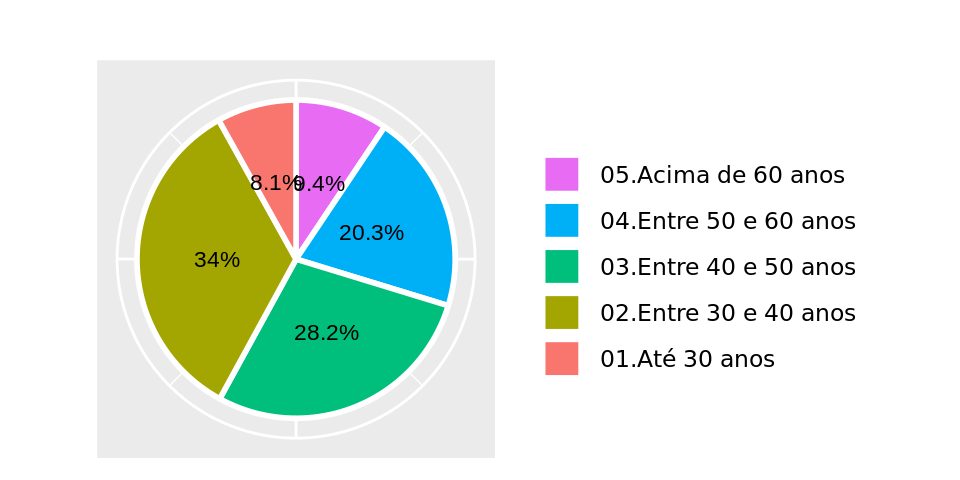
\includegraphics{ebookrnp_files/figure-latex/graf01-1} 

}

\caption{Gráfico de setores para faixa de idade dos docentes}\label{fig:graf01}
\end{figure}

Como podemos notar, a figura \ref{fig:graf01} é muito intuitiva para representar visualmente a distribuição de frequências das classes de uma variável categórica. Combinado com as cores de cada fatia, fica claro e objetivo a parcela de cada categoria para explicar o todo que por sua vez representa 100\%.

\hypertarget{barras}{%
\subsubsection{Barras}\label{barras}}

Gráficos de barras também são intuitivos e geralmente são preferíveis em relação aos gráficos de setores. Isso ocorre porque o olho humano é mais sensível a linhas do que círculos e formas em 3D e prefere analisar figuras mais limpas. Para expandir seus conhecimentos sobre análise visual, sugerimos a \citep{tufte2014visual}.

\begin{Shaded}
\begin{Highlighting}[]
\NormalTok{p <-}\StringTok{ }\NormalTok{ggplot2}\OperatorTok{::}\KeywordTok{ggplot}\NormalTok{(tb, }\KeywordTok{aes}\NormalTok{(classe, fr, }\DataTypeTok{fill =}\NormalTok{ classe))}
\NormalTok{p }\OperatorTok{+}\StringTok{ }\NormalTok{ggplot2}\OperatorTok{::}\KeywordTok{geom_bar}\NormalTok{(}\DataTypeTok{width =} \DecValTok{1}\NormalTok{, }\DataTypeTok{size =} \DecValTok{1}\NormalTok{, }\DataTypeTok{color =} \StringTok{"white"}\NormalTok{, }
                      \DataTypeTok{stat =} \StringTok{"identity"}\NormalTok{, }\DataTypeTok{show.legend =} \OtherTok{FALSE}\NormalTok{) }\OperatorTok{+}
\StringTok{  }\NormalTok{ggplot2}\OperatorTok{::}\KeywordTok{geom_text}\NormalTok{(}\KeywordTok{aes}\NormalTok{(}\DataTypeTok{label =} \KeywordTok{paste0}\NormalTok{(}\KeywordTok{round}\NormalTok{(}\DecValTok{100}\OperatorTok{*}\NormalTok{fr, }\DecValTok{1}\NormalTok{), }\StringTok{"%"}\NormalTok{)),}
                     \DataTypeTok{position =} \KeywordTok{position_stack}\NormalTok{(}\DataTypeTok{vjust =} \DecValTok{1}\NormalTok{), }\DataTypeTok{size=}\DecValTok{3}\NormalTok{) }\OperatorTok{+}
\StringTok{  }\NormalTok{ggplot2}\OperatorTok{::}\KeywordTok{labs}\NormalTok{(}\DataTypeTok{x =} \OtherTok{NULL}\NormalTok{, }\DataTypeTok{y =} \OtherTok{NULL}\NormalTok{, }\DataTypeTok{fill =} \OtherTok{NULL}\NormalTok{, }\DataTypeTok{title =} \StringTok{""}\NormalTok{) }\OperatorTok{+}
\StringTok{  }\NormalTok{ggplot2}\OperatorTok{::}\KeywordTok{theme_gray}\NormalTok{() }\OperatorTok{+}\StringTok{ }\KeywordTok{coord_flip}\NormalTok{() }\OperatorTok{+}
\StringTok{  }\NormalTok{ggplot2}\OperatorTok{::}\KeywordTok{theme}\NormalTok{(}\DataTypeTok{axis.line =} \KeywordTok{element_blank}\NormalTok{())}
\end{Highlighting}
\end{Shaded}

\begin{figure}[H]

{\centering 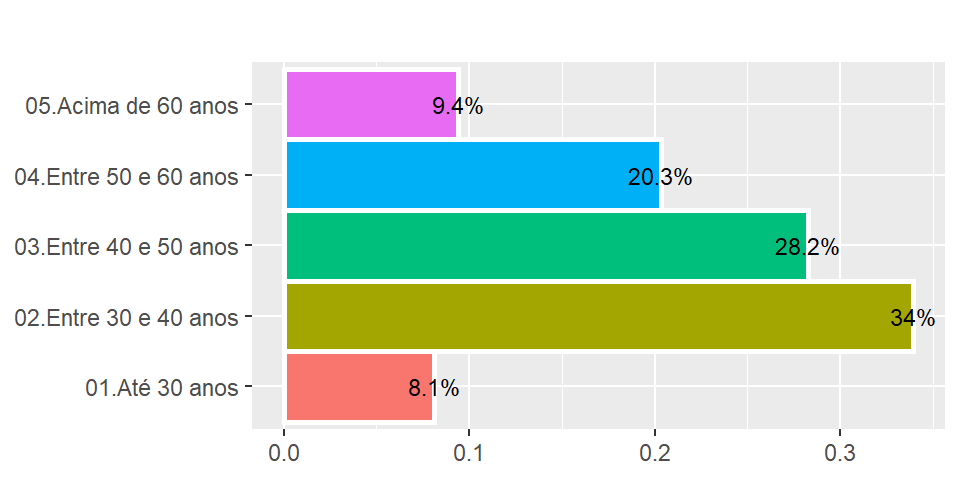
\includegraphics{ebookrnp_files/figure-latex/graf02-1} 

}

\caption{Gráfico de barras para faixa de idade dos docentes}\label{fig:graf02}
\end{figure}

A figura \ref{fig:graf02} mostra um gráfico de barras para as faixas de idade dos docentes, nele pode-se notar que visualmente as diferenças de patemares ficam evidentes mesmo sem ter a informação em percentual em cada barra. Com isso a leitura fica mais direta e é possível comparar todas as barras simultaneamente. O eixo y contém as proporções e o eixo x a descrição de cada categoria.

\hypertarget{grafico-para-duas-variaveis-categoricas}{%
\subsection{Gráfico para duas variáveis categóricas}\label{grafico-para-duas-variaveis-categoricas}}

Vimos nas tabelas de frequência que as tabelas de dupla entrada são boas ferramentas para analisar conjuntamente a relação entre duas variáveis, mas isso também pode ser feito de forma visual.

\hypertarget{mosaicplot}{%
\subsubsection{\texorpdfstring{\emph{mosaicplot}}{mosaicplot}}\label{mosaicplot}}

Podemos visualizar a relação entre duas variáveis categóricas ou numéricas de poucas classes, através do \textbf{Gráfico de mosaico (\emph{mosaic plot})}. O pacote \texttt{ggmosaic} expande o \texttt{ggplot2} para produzir este tipo de gráfico.

\begin{Shaded}
\begin{Highlighting}[]
\NormalTok{p <-}\StringTok{ }\NormalTok{ggplot2}\OperatorTok{::}\KeywordTok{ggplot}\NormalTok{(base_docentes)}
\NormalTok{p }\OperatorTok{+}\StringTok{ }\NormalTok{ggplot2}\OperatorTok{::}\KeywordTok{theme_gray}\NormalTok{() }\OperatorTok{+}
\StringTok{  }\NormalTok{ggmosaic}\OperatorTok{::}\KeywordTok{geom_mosaic}\NormalTok{(}\KeywordTok{aes}\NormalTok{(}\DataTypeTok{x =} \KeywordTok{product}\NormalTok{(sexo), }\DataTypeTok{fill =}\NormalTok{ faixaIdade), }
                        \DataTypeTok{show.legend =} \OtherTok{FALSE}\NormalTok{) }\OperatorTok{+}
\StringTok{  }\NormalTok{ggplot2}\OperatorTok{::}\KeywordTok{labs}\NormalTok{(}\DataTypeTok{x =} \OtherTok{NULL}\NormalTok{, }\DataTypeTok{y =} \OtherTok{NULL}\NormalTok{, }\DataTypeTok{fill =} \OtherTok{NULL}\NormalTok{, }\DataTypeTok{title =} \StringTok{""}\NormalTok{) }\OperatorTok{+}
\StringTok{  }\NormalTok{ggplot2}\OperatorTok{::}\KeywordTok{theme}\NormalTok{(}\DataTypeTok{axis.line =} \KeywordTok{element_blank}\NormalTok{())}
\end{Highlighting}
\end{Shaded}

\begin{figure}[H]

{\centering 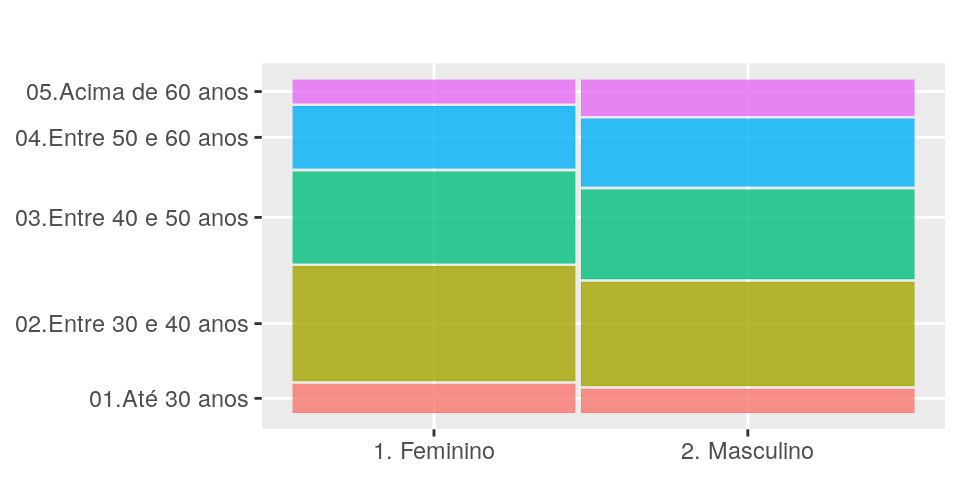
\includegraphics{ebookrnp_files/figure-latex/graf03-1} 

}

\caption{Gráfico de mosaico para faixa de idade dos docentes por sexo}\label{fig:graf03}
\end{figure}

Cada coluna da figura \ref{fig:graf03} representa uma classe da variável sexo do docente e cada linha representa a uma classe da variável faixa de idade. Note que o cruzamento dente linhas e colunas geram retângulos que estimam a frequência de de cada cruzamento, sendo maior nos casos em que existem mais dados. Por exemplo, proporcionalmente docentes do sexo masculino acima de 60 anos são maioria nesta faixa de idade. Aliás, gráfico mostra que a proporção de docentes do sexo masculino é maior do que o feminino em todas as faixas de idade.

\hypertarget{exercicios}{%
\subsection{Exercícios}\label{exercicios}}

Para resolver os exercícios desta seção, utilize o conjunto de dados \texttt{DM\_CURSO.CSV} presente na pasta de dados. Esta base de dados possui informações sobre os cursos das IES no censo de 2017 do INEP. Mais informações sobre as variáveis podem ser obtidas no dicionario de dados presente na pasta \texttt{AJUDA/ANEXOS}.

\begin{Shaded}
\begin{Highlighting}[]
\NormalTok{classes <-}\StringTok{ }\NormalTok{rnp}\OperatorTok{::}\KeywordTok{rnp_get_classes_inep}\NormalTok{(}\DataTypeTok{caminho =}\NormalTok{ dicionario, }
                                     \DataTypeTok{aba =} \StringTok{"DM_CURSO"}\NormalTok{, }
                                     \DataTypeTok{retorna_lista =} \OtherTok{FALSE}\NormalTok{)}
\CommentTok{# Base de dados  }
\NormalTok{base <-}\StringTok{ }\NormalTok{rnp}\OperatorTok{::}\KeywordTok{rnp_read}\NormalTok{(}\DataTypeTok{base =} \StringTok{"Dados/INEP/DADOS/DM_CURSO.CSV"}\NormalTok{,}
                      \DataTypeTok{sep =} \StringTok{"|"}\NormalTok{, }
                      \DataTypeTok{dec =} \StringTok{"."}\NormalTok{, }
                      \DataTypeTok{header =} \OtherTok{TRUE}\NormalTok{, }
                      \DataTypeTok{encoding =} \StringTok{"Latin-1"}\NormalTok{,}
                      \DataTypeTok{verbose =} \OtherTok{FALSE}\NormalTok{, }
                      \DataTypeTok{showProgress =} \OtherTok{FALSE}\NormalTok{)}
\CommentTok{# Aplica classes}
\NormalTok{base_curso <-}\StringTok{ }\NormalTok{rnp}\OperatorTok{::}\KeywordTok{rnp_aplica_classes}\NormalTok{(}\DataTypeTok{base =}\NormalTok{ base, }\DataTypeTok{classes =}\NormalTok{ classes)}
\CommentTok{# Verifica algumas propriedades das 10 primeiras colunas.}
\NormalTok{dplyr}\OperatorTok{::}\KeywordTok{glimpse}\NormalTok{(base_curso[,}\DecValTok{1}\OperatorTok{:}\DecValTok{10}\NormalTok{])}
\end{Highlighting}
\end{Shaded}

\begin{verbatim}
## Observations: 35,693
## Variables: 10
## $ NU_ANO_CENSO            <int> 2017, 2017, 2017, ...
## $ CO_IES                  <int> 789, 4567, 2341, 6...
## $ CO_LOCAL_OFERTA         <int> 1033528, 659871, 1...
## $ CO_UF                   <int> 14, 51, 35, 35, 53...
## $ CO_MUNICIPIO            <int> 1400100, 5107925, ...
## $ CO_CURSO                <int> 1259131, 1258115, ...
## $ NO_CURSO                <chr> "MÚSICA", "GESTÃO ...
## $ CO_OCDE_AREA_GERAL      <int> 1, 3, 3, 5, 3, 7, ...
## $ CO_OCDE_AREA_ESPECIFICA <int> 14, 34, 38, 52, 38...
## $ CO_OCDE_AREA_DETALHADA  <int> 146, 345, 380, 522...
\end{verbatim}

\BeginKnitrBlock{exercise}
\protect\hypertarget{exr:unnamed-chunk-37}{}{\label{exr:unnamed-chunk-37} }TODO, TODO, TODO
\EndKnitrBlock{exercise}

\hypertarget{variaveis-numericas}{%
\section{Variáveis numéricas}\label{variaveis-numericas}}

Variáveis numéricas são se longe o tipo mais comum e analisável de dados, pois contemplam medidas de todo tipo de processo. Por exemplo, idade de uma pessoa em dias, peso, altura, total de pessoas em um metrô, em uma fila de cinema e por aí vai. Por permitir cálculos matemáticos, este tipo de variável tem sido estudado há milênios e portanto, boa parte das técnicas estatísticas atuais de baseiam em dados numéricos. Neste tópico abordaremos as principais medidas estatísticas cobrindo centralidade, dispersão entre outras e os principais gráficos que podem ser empregados.

\hypertarget{medidas-estatisticas-de-centraliade}{%
\subsection{Medidas estatísticas de centraliade}\label{medidas-estatisticas-de-centraliade}}

Quando olhamos um conjunto de dados de uma variável numérica logo pensamos em alguma forma de resumir estes dados para gerar algum tipo de informação. As medidas estatísticas de centralidade representam resumos numéricos que apontam para o centro do conjunto de dados. A figura \ref{fig:fig06} ilustra bem a ideia e também indica uma vulnerabilidade da \textbf{média} que são os extremos. Pontos extremos podem inserir viés no valor e na interpretação de uma média, mas para complementar a média temos a \textbf{mediana}, \textbf{moda} e \textbf{quartis} que veremos nos tópicos a seguir.

\begin{figure}[H]

{\centering 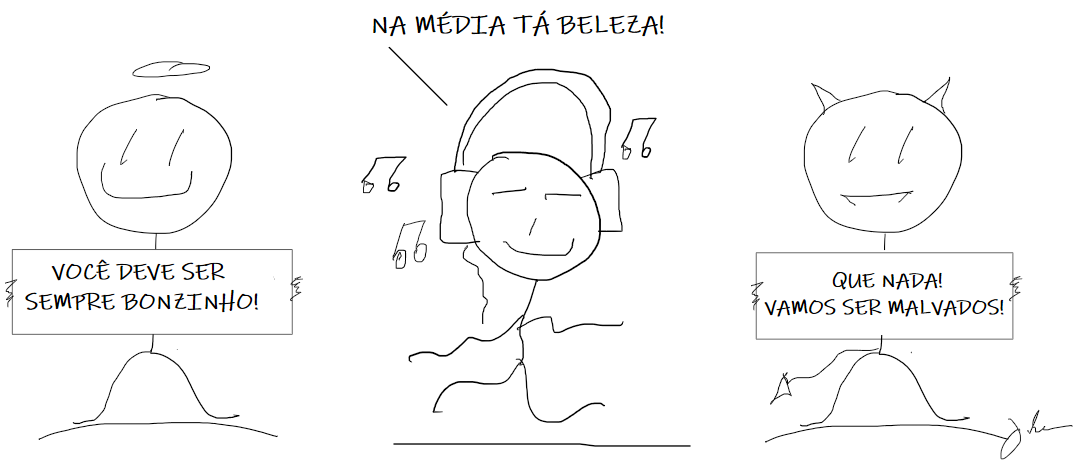
\includegraphics[width=1\linewidth]{../Imagens/ebook_anima_06} 

}

\caption{Na média, tudo bem}\label{fig:fig07}
\end{figure}

\begin{quote}
As medidas estatísticas descritas nesta seção são aplicadas a conjuntos de dados (amostras e populações) e também a distribuições de probabilidade. Para manter o tero prático deste texto, vamos focar em dados. No capitulo sobre probabilidade retornaremos o assunto no contexto das distribuições de probabilidade.
\end{quote}

\hypertarget{media-bar-x-mu}{%
\subsubsection{\texorpdfstring{Média (\(\bar X, \mu\))}{Média (\textbackslash{}bar X, \textbackslash{}mu)}}\label{media-bar-x-mu}}

Existem muitos tipos de média como por exemplo aritmética, ponderada, geométrica e a harmônica. Em qualquer uma delas, o intuito é resumir a centralidade dos dados em relação a seus extremos dando mais ou menos peso para cada observação. Representamos a média de uma amostra pela letra latina \(\bar X\) (xis-barra) e a média populacional pela letra grega \(\mu\) e calculamos com a mesma expressão matemática.

\begin{quote}
Veremos no capítulo sobre teoria das probabilidades que a média de uma veriável aleatória \(X\) é chamada de \textbf{valor esperado ou esperança (\(E[X]\))}.
\end{quote}

\textbf{Média aritmética}: é a soma de todos os valores e dividido pelo total deles. Ou seja, o resultado dessa divisão equivale a um valor médio entre todos os valores e é calculada por:

\[\bar X = \frac{x_1 + x_2 + x_3 + \dots + x_n}{n}, i = 1, 2, 3, \dots, n\]

onde \(x_1, x_2, x_3, \dots, x_n\) representam cada valor correspondente a um elemento \(i\) da amostra e \(n\) o total de elementos.

\begin{quote}
Este tipo de média é aplicado preferecialmente quando cada elemento tem peso igual a uma unidade, ou seja, quando não houver muita repetição.
\end{quote}

\BeginKnitrBlock{example}
\protect\hypertarget{exm:unnamed-chunk-38}{}{\label{exm:unnamed-chunk-38} }Com base no conjunto de dados de IES, vamos calcular algumas médias.
\EndKnitrBlock{example}

\begin{Shaded}
\begin{Highlighting}[]
\NormalTok{base_ies }\OperatorTok\StringTok{ }
\StringTok{  }\NormalTok{dplyr}\OperatorTok{::}\KeywordTok{summarise}\NormalTok{(}\StringTok{`}\DataTypeTok{Total técnicos}\StringTok{`}\NormalTok{  =}\StringTok{ }\KeywordTok{mean}\NormalTok{(TotalTecnicos),}
                   \StringTok{`}\DataTypeTok{Receita própria` = mean(ReceitaPropria),}
\DataTypeTok{                   }\StringTok{`}\NormalTok{Depesa pesquisa}\StringTok{`}\DataTypeTok{ = mean(DespesaPesquisa)) %>% }
\DataTypeTok{  knitr::kable(caption = "Média anual para dados de IES", format = tb_formata) %>% }
\DataTypeTok{  kableExtra::kable_styling(latex_options = "hold_position")}
\end{Highlighting}
\end{Shaded}

\begin{table}[!h]

\caption{\label{tab:tab06}Média anual para dados de IES}
\centering
\begin{tabular}{r|r|r}
\hline
Total técnicos & Receita própria & Depesa pesquisa\\
\hline
168.1 & 145378180 & 886404\\
\hline
\end{tabular}
\end{table}

A tabela \ref{tab:tab06} mostra que a média da receita própria anual das IES brasileiras, segundo o censo de 2017, foi de R\$ 143.468.742. Este valor parece um pouco suspeito, pois representa 85,76\% do PIB (Produto Interno Bruto) do estado de pernambuco tendo 2018 como ano base, segundo dados do IBGE. Mas vamos entender adiante como investigar isso melhor.

\textbf{Média aritmética ponderada}: Neste caso, é assumido que cada elemento amostral tem um peso, então a média aritmética ponderada é calculada multiplicando cada valor do conjunto de dados pelo seu peso, somando tudo e dividindo pela soma de todos os pesos. Na verdade a média aritmética simples é um caso especial da ponderada quando cada peso vale 1. A média ponderada é dada por:

\[\bar X_p = \frac{p_1 \times x_1 + p_2 \times x_2 + p_3\times  x_3 + \dots + p_n \times x_n}{p_1 + p_2 + p_3 + \dots + p_n}, i = 1, 2,3 \dots, n\]

sendo \(x_1, x_2, x_3, \dots , x_n\) cada valor associado a um \(i-ésimo\) elemento da amostra e \(p_1 + p_2 + p_3 + \dots + p_n\) cada peso relacionado com cada elemento da amostra.

\begin{quote}
Quando a amostra possuir muitas repetições ou precisar ser balizada por algum peso, esta média é mais recomendada.
\end{quote}

\BeginKnitrBlock{example}
\protect\hypertarget{exm:unnamed-chunk-39}{}{\label{exm:unnamed-chunk-39} }Com base no conjunto de dados de IES, vamos calcular a média da receita própria ponderada pelo total de técnicos.
\EndKnitrBlock{example}

\begin{Shaded}
\begin{Highlighting}[]
\NormalTok{base_ies }\OperatorTok\StringTok{ }
\StringTok{  }\NormalTok{dplyr}\OperatorTok{::}\KeywordTok{summarise}\NormalTok{(}\StringTok{`}\DataTypeTok{Receita própria`  = mean(ReceitaPropria),}
\DataTypeTok{            }\StringTok{`}\NormalTok{Receita própria ponderada}\StringTok{`}\DataTypeTok{ = weighted.mean(x = ReceitaPropria,}
\DataTypeTok{                                                        w = TotalTecnicos)) %>% }
\DataTypeTok{  knitr::kable(format = tb_formata,}
\DataTypeTok{               caption = "Média receita própria ponderada pelo total de técnicos") %>% }
\DataTypeTok{  kableExtra::kable_styling(latex_options = "hold_position")}
\end{Highlighting}
\end{Shaded}

\begin{table}[!h]

\caption{\label{tab:tab07}Média receita própria ponderada pelo total de técnicos}
\centering
\begin{tabular}{r|r}
\hline
Receita própria & Receita própria ponderada\\
\hline
145378180 & 229043797\\
\hline
\end{tabular}
\end{table}

Note da tabela \ref{tab:tab07} que a média ponderada é maior que a aritmética da tabela \ref{tab:tab06} e isso ocorre porque IES maiores possuem mais receita e sendo esta ponderada por um volume maior de técnicos faz com que a média suba.

A médias geométrica é mais rara, porém existem aplicações em áreas como ciências sociais como formas de estivar a expectativa de vida ao nascer, na economia como indicadores financeiros e na geometria. Assim como a média geométrica, a harmônica também é rara e possui aplicações na área da física em situações que envolvem taxas. Fica ao cargo do leitor interessado pesquisar mais sobre estas médias.

\hypertarget{mediana-m_d}{%
\subsubsection{\texorpdfstring{Mediana (\(M_d\))}{Mediana (M\_d)}}\label{mediana-m_d}}

Para compreender melhor o conceito de mediana é importante saber que ela depende da ordenação de forma crescente dos dados da variável numérica. Como se trata de números, ao ordenar os dados podemos trazer a ideia de centro. A mediana é uma medida estatística que calcula o valor central dos dados de forma que se tenha metade dos valores abaixo e metade acima da mediana. Resumindo, mediana é o valor do meio do conjunto de dados.

\begin{quote}
Quando o conjunto de dados tiver um número impar de observações, a media será o valor central e quando o comprimento for par, a mediana será a média dos dois elementos centrais. A mediana também é conhecida como uma medida resistente a pontos discrepantes.
\end{quote}

\BeginKnitrBlock{example}
\protect\hypertarget{exm:unnamed-chunk-40}{}{\label{exm:unnamed-chunk-40} }No conjunto de dados \texttt{c(0,\ 1,\ 2,\ 3,\ 4,\ 5,\ 6)} qual é a mediana?
\EndKnitrBlock{example}

Neste caso a mediana é 3, porque a amostra tem tamanho 7 e 3 é o elemento que separa os dados 50\% / 50\%. No R utilizamos a função \texttt{median()} para calcular a médiana.

\begin{Shaded}
\begin{Highlighting}[]
\NormalTok{x <-}\StringTok{ }\KeywordTok{c}\NormalTok{(}\DecValTok{0}\NormalTok{, }\DecValTok{1}\NormalTok{, }\DecValTok{2}\NormalTok{, }\DecValTok{3}\NormalTok{, }\DecValTok{4}\NormalTok{, }\DecValTok{5}\NormalTok{, }\DecValTok{6}\NormalTok{)}
\KeywordTok{median}\NormalTok{(x, }\DataTypeTok{na.rm =} \OtherTok{TRUE}\NormalTok{)}
\end{Highlighting}
\end{Shaded}

\begin{verbatim}
## [1] 3
\end{verbatim}

\begin{Shaded}
\begin{Highlighting}[]
\CommentTok{# OBS: na.rm remove elementos nulos da amostra, quando existirem}
\end{Highlighting}
\end{Shaded}

\BeginKnitrBlock{example}
\protect\hypertarget{exm:unnamed-chunk-42}{}{\label{exm:unnamed-chunk-42} }No conjunto de dados \texttt{c(2,\ 3,\ 4,\ 5,\ 6,\ 7)} qual é a mediana?
\EndKnitrBlock{example}

Neste caso a mediana é \(\frac{4 + 5}{2} = 4.5\), porque a amostra tem tamanho 6 e sendo que 4 e 5 são os elementos que estão no centro.

\begin{Shaded}
\begin{Highlighting}[]
\NormalTok{x <-}\StringTok{ }\KeywordTok{c}\NormalTok{(}\DecValTok{2}\NormalTok{, }\DecValTok{3}\NormalTok{, }\DecValTok{4}\NormalTok{, }\DecValTok{5}\NormalTok{, }\DecValTok{6}\NormalTok{, }\DecValTok{7}\NormalTok{)}
\KeywordTok{median}\NormalTok{(x, }\DataTypeTok{na.rm =} \OtherTok{TRUE}\NormalTok{)}
\end{Highlighting}
\end{Shaded}

\begin{verbatim}
## [1] 4.5
\end{verbatim}

\hypertarget{moda-m_o}{%
\subsubsection{\texorpdfstring{Moda (\(M_o\))}{Moda (M\_o)}}\label{moda-m_o}}

A moda é uma medida estatística que aponta quem são os valores mais frequentes numa amostra com elementos repetidos sendo ela o valor que ocorre com maior frequência ou o valor mais comum. Quando os dados são numéricos e já estão agrupados em classes, chamamos a classe com maior frequência de \textbf{classe modal} e seu valor é determinado pela média dos seus extremos.

\begin{quote}
Diferentemente da média e mediana já vistas, a moda também se aplica a variáveis categóricas, uma vez que serve para identificar as classes ou valores mais frequentes.
\end{quote}

Quando uma amostra possui apenas uma moda diz-se que ele é \emph{unimodal}, sem tem duas é \emph{bimodal} e se tem três ou mais é dita \emph{multimodal}.

\begin{Shaded}
\begin{Highlighting}[]
\NormalTok{knitr}\OperatorTok{::}\KeywordTok{kable}\NormalTok{(rnp}\OperatorTok{::}\KeywordTok{rnp_freq}\NormalTok{(base_docentes}\OperatorTok{$}\NormalTok{idade), }
             \DataTypeTok{digits =} \DecValTok{3}\NormalTok{,}
             \DataTypeTok{booktabs =} \OtherTok{TRUE}\NormalTok{,}
             \DataTypeTok{format =}\NormalTok{ tb_formata,}
             \DataTypeTok{caption =} \StringTok{"Frequências para idade dos docentes das IES"}\NormalTok{) }\OperatorTok\StringTok{ }
\StringTok{  }\NormalTok{kableExtra}\OperatorTok{::}\KeywordTok{kable_styling}\NormalTok{(}\DataTypeTok{latex_options =} \StringTok{"hold_position"}\NormalTok{)}
\end{Highlighting}
\end{Shaded}

\begin{table}[!h]

\caption{\label{tab:tab08}Frequências para idade dos docentes das IES}
\centering
\begin{tabular}{lrrrr}
\toprule
classe & fa & fr & Faa & Fra\\
\midrule
19--36 & 107295 & 0.274 & 107295 & 0.274\\
36--43 & 95550 & 0.244 & 202845 & 0.517\\
43--52 & 92360 & 0.236 & 295205 & 0.753\\
52--99 & 96831 & 0.247 & 392036 & 1.000\\
\bottomrule
\end{tabular}
\end{table}

Na tabela \ref{tab:tab08} vemos que a classe modal é a que contém idades entre 20 e 36 anos, pois ela representa 28,6\% da amostra. Com base na classe modal, temos que \(M_o = \frac{36+20}{2} = 28\) anos.

\BeginKnitrBlock{example}
\protect\hypertarget{exm:unnamed-chunk-44}{}{\label{exm:unnamed-chunk-44} }Dadas as amostras genéricas \texttt{x\ =\ \{2,\ 5,\ 3,\ 4,\ 4\},\ y\ =\ \{5,5,7,7,6,1,2,1\},\ z\ =\ \{9,1,7,8,4\}} determine, quando existir e moda e sua classificação.
\EndKnitrBlock{example}

Uma forma de verificar se um conjunto de dados possui moda é verificar se tem algum valor que se repete ao longo da amostra. Isso pode ser feito através das funções \texttt{table()} e \texttt{duplicated()}. Enquanto a primeira faz uma tabulação dos valores ou das classes, a segunda varre a variável buscando quem são os valores que ocorrem mais de uma veze retornando \texttt{TRUE}, caso algum se repita. Vejamos a solução.

\begin{Shaded}
\begin{Highlighting}[]
\CommentTok{# Preparando os dados como vetores através da função c() e ordenando com sort()}
\NormalTok{x <-}\StringTok{ }\KeywordTok{sort}\NormalTok{(}\KeywordTok{c}\NormalTok{(}\DecValTok{2}\NormalTok{, }\DecValTok{5}\NormalTok{, }\DecValTok{3}\NormalTok{, }\DecValTok{4}\NormalTok{, }\DecValTok{4}\NormalTok{))}
\KeywordTok{paste}\NormalTok{(}\StringTok{"x possui"}\NormalTok{, x[}\KeywordTok{duplicated}\NormalTok{(x)], }\StringTok{"como moda"}\NormalTok{)}
\end{Highlighting}
\end{Shaded}

\begin{verbatim}
## [1] "x possui 4 como moda"
\end{verbatim}

\begin{Shaded}
\begin{Highlighting}[]
\CommentTok{# x é unimodal}

\NormalTok{y <-}\StringTok{ }\KeywordTok{sort}\NormalTok{(}\KeywordTok{c}\NormalTok{(}\DecValTok{5}\NormalTok{,}\DecValTok{5}\NormalTok{,}\DecValTok{7}\NormalTok{,}\DecValTok{7}\NormalTok{,}\DecValTok{6}\NormalTok{,}\DecValTok{1}\NormalTok{,}\DecValTok{2}\NormalTok{,}\DecValTok{1}\NormalTok{))}
\KeywordTok{paste}\NormalTok{(}\StringTok{"y possui"}\NormalTok{, y[}\KeywordTok{duplicated}\NormalTok{(y)], }\StringTok{"como moda"}\NormalTok{)}
\end{Highlighting}
\end{Shaded}

\begin{verbatim}
## [1] "y possui 1 como moda" "y possui 5 como moda"
## [3] "y possui 7 como moda"
\end{verbatim}

\begin{Shaded}
\begin{Highlighting}[]
\CommentTok{# y é multimodal}

\NormalTok{z <-}\StringTok{ }\KeywordTok{sort}\NormalTok{(}\KeywordTok{c}\NormalTok{(}\DecValTok{9}\NormalTok{,}\DecValTok{1}\NormalTok{,}\DecValTok{7}\NormalTok{,}\DecValTok{8}\NormalTok{,}\DecValTok{4}\NormalTok{))}
\KeywordTok{paste}\NormalTok{(}\StringTok{"z possui"}\NormalTok{, z[}\KeywordTok{duplicated}\NormalTok{(z)], }\StringTok{"como moda"}\NormalTok{)}
\end{Highlighting}
\end{Shaded}

\begin{verbatim}
## [1] "z possui  como moda"
\end{verbatim}

\begin{Shaded}
\begin{Highlighting}[]
\CommentTok{# z não possui moda.}
\end{Highlighting}
\end{Shaded}

As medidas de centralidade de forma geral sempre buscarão representar quais dados estão no centro ou apontando para mesmo no conjunto de dados.
A figura \ref{fig:fig08} exemplifica um conjunto de medidas em uma linha onde a média representa o centro e os pontos as possíveis medidas realizadas.

\begin{figure}[H]

{\centering 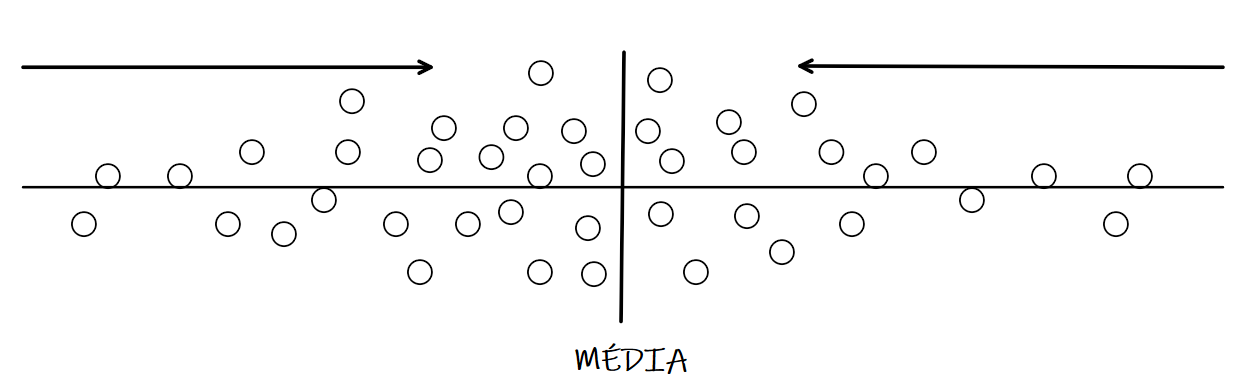
\includegraphics[width=1\linewidth]{../Imagens/ebook_anima_07} 

}

\caption{Centralidade}\label{fig:fig08}
\end{figure}

\hypertarget{medidas-estatisticas-de-dispersao}{%
\subsection{Medidas estatísticas de dispersão}\label{medidas-estatisticas-de-dispersao}}

De forma simples, podemos entender medidas de dispersão como estatísticas que medem o quanto os dados estão espalhados. Desta forma, este tipo de medida é zero se os dados são todos iguais e vai aumentanto à medida em que a diversidade dos dados aumenta.
Estatísticas de dispersão são muito aplicadas em área como física ajuando a medir a variabilidade de medições feitas em experimentos; nas ciências biológicas estimando a variabilidade \textbf{interindivíduos} (membros distintos da mesma amostra são diferentes uns dos outros) e \textbf{intraindivíduos} (um mesmo individuos submetido a algum teste em condições distintas poduzem resultados diferentes) e em muitos ramos das ciências como economia, medicina e engenharia.
As principais medidas estatísticas de dispersão são \textbf{Desvio padrão (\(S,\sigma\)) e Variância (\(S^2,\sigma^2\)), Amplitude, Desvio absoluto e Coeficiente de variação}

\hypertarget{desvio-padrao-ssigma-e-variancia-s2sigma2}{%
\subsubsection{\texorpdfstring{Desvio padrão (\(S,\sigma\)) e variância (\(S^2,\sigma^2\))}{Desvio padrão (S,\textbackslash{}sigma) e variância (S\^{}2,\textbackslash{}sigma\^{}2)}}\label{desvio-padrao-ssigma-e-variancia-s2sigma2}}

Desvio padrão e variância são medidas que buscam estimar a dispersão dos dados em torno da sua média. Quando estamos falando de população temos o \textbf{desvio padrão ou variância populacional}, representados pela letra grega minúscula \(\sigma\) para desvio padrão e \(\sigma^2\) para variância. No caso de amostra, representamos pela letra latina \(S\) para o primeiro e \(S^2\) para o segundo caso.

O desvio padrão populacional é dado por:

\[{\displaystyle \sigma ={\sqrt {{\frac {1}{N}}\sum _{i=1}^{N}(X_{i}-\mu )^{2}}}}\]

em que \(X_i,i=1,2,...,N\) são os elementos da população e \(\mu\) é a média populacional.

O devio padrão amostral é dado por:

\[{\displaystyle S_{n-1}={\sqrt {{\frac {1}{n-1}}\sum _{i=1}^{n}(X_{i}-{\overline {X}})^{2}}}}\]

em que \(X_i,i=1,2,...,n\) são os elementos da amostra e \(\bar X\) é a média amostral.

\begin{quote}
O denominador do desvio padrão amostral é \(n-1\) em vez de \(n\). Este fator de correção é conhecido como correção de Bessel \citep{reichmann1961use} e é aplicado porque no cálculo da média a partir da amostra, perde-se um \textbf{grau de liberdade}. Grau de liberdade refere-se ao total de elementos da amostra supondo que cada um é independente do outro. Como \(S\) utiliza \(\bar X\) que por sua vez está ligada com cada elemento da amostra, há epenas \(n-1\) elementos independentes após \(\bar X\) ser calculado.
\end{quote}

A variância é o quadrado do desvio padão. Assim:

Variância populacional é dada por

\[\sigma^2 ={{\frac {1}{N}}\sum _{i=1}^{N}(X_{i}-\mu )^{2}}\]

e a variância amostral por:

\[S_{n-1}={{\frac {1}{n-1}}\sum _{i=1}^{n}(X_{i}-{\overline {X}})^{2}}\]

Em R calculamos o desvio padrão de uma variável com a função \texttt{sd()} e a variância com a função \texttt{var()}.

\BeginKnitrBlock{example}
\protect\hypertarget{exm:unnamed-chunk-46}{}{\label{exm:unnamed-chunk-46} }Calcule a média, desvio padrão e a variância da idade dos docentes das IES.
\EndKnitrBlock{example}

\begin{Shaded}
\begin{Highlighting}[]
\NormalTok{base_docentes }\OperatorTok\StringTok{ }
\StringTok{  }\NormalTok{dplyr}\OperatorTok{::}\KeywordTok{summarise}\NormalTok{(}\StringTok{`}\DataTypeTok{Média}\StringTok{`}\NormalTok{ =}\StringTok{ }\KeywordTok{mean}\NormalTok{(idade),}
                   \StringTok{`}\DataTypeTok{Desvio padrão}\StringTok{`}\NormalTok{ =}\StringTok{ }\KeywordTok{sd}\NormalTok{(idade),}
                   \StringTok{`}\DataTypeTok{Variância}\StringTok{`}\NormalTok{ =}\StringTok{ }\KeywordTok{var}\NormalTok{(idade))}
\end{Highlighting}
\end{Shaded}

\begin{verbatim}
## # A tibble: 1 x 3
##   Média `Desvio padrão` Variância
##   <dbl>           <dbl>     <dbl>
## 1  44.5            11.0      120.
\end{verbatim}

ou diretamente com.

\begin{Shaded}
\begin{Highlighting}[]
\KeywordTok{paste}\NormalTok{(}\StringTok{"Desvio padrão ="}\NormalTok{, }\KeywordTok{round}\NormalTok{(}\KeywordTok{sd}\NormalTok{(base_docentes}\OperatorTok{$}\NormalTok{idade), }\DecValTok{3}\NormalTok{))}
\end{Highlighting}
\end{Shaded}

\begin{verbatim}
## [1] "Desvio padrão = 10.963"
\end{verbatim}

\begin{Shaded}
\begin{Highlighting}[]
\KeywordTok{paste}\NormalTok{(}\StringTok{"Variância ="}\NormalTok{, }\KeywordTok{round}\NormalTok{(}\KeywordTok{var}\NormalTok{(base_docentes}\OperatorTok{$}\NormalTok{idade), }\DecValTok{3}\NormalTok{))}
\end{Highlighting}
\end{Shaded}

\begin{verbatim}
## [1] "Variância = 120.181"
\end{verbatim}

\begin{itemize}
\tightlist
\item
  \textbf{Interpretação do desvio padrão}: No exemplo acima vemos que a média de idade dos docentes é de 44,2 anos com desvio padrão de 11 e variância de 120, mas o que isso significa? - A variância de idade é uma medida cuja unidade de media é \(ano^2\). Ano ao quadrado não tem interpretação direta então utilizamos o desvio padrão. Em garal quanto maior o desvio padrão mais espalhados estão os dados em relação à media. Não é conhecida uma regra generalizada para dizer se um desvio padrão é menor ou maior, porém, com base na teoria das probabilidades temos uma regra de ouro que é aplicada sempre que a curva dos dados segue uma distribuição Normal (por hora, epenas aceite, veremos ela mais adiante!).
\end{itemize}

\begin{figure}[H]

{\centering 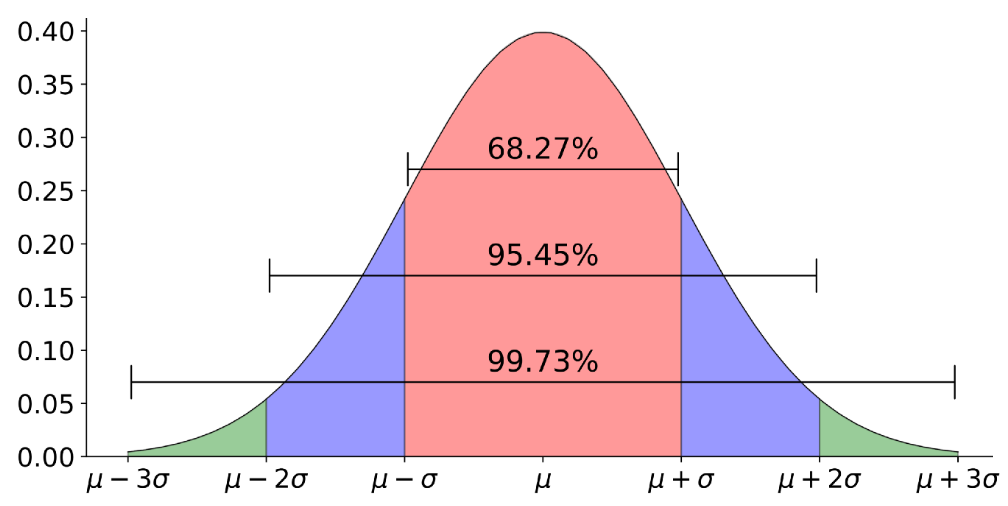
\includegraphics[width=1\linewidth]{../Imagens/ebook_normal} 

}

\caption{Centralidade}\label{fig:fig09}
\end{figure}

Conforme vemos na figura \ref{fig:fig09}, em torno da média mais ou menos um desvio padrão devem estar 68,27\% dos dados, já entre a média mais ou menos 2 desvios padrão deve estar 95,45\% dos dados. Seguindo esta lógica, a interpretação deve levar em conta a distribuição dos dados e a precisão que o experimento ou estudo exige. Assim, sendo no nosso exemplo a média de idade dos docentes é 44,2 então entre \(44,2 \pm 11 = (33.4-55.4)\) devem estar 68,27\% dos docentes.

\hypertarget{amplitude}{%
\subsubsection{Amplitude}\label{amplitude}}

A amplitude de um conjunto de dados ordenado é a distância entre o menor e o maior valor. Na figura \ref{fig:fig08} se seus valores estiverem ordenados do maior para o menor, a amplitude seria o ponto mais à direita \textbf{Máximo} menos o ponto mais à esquerda \textbf{Mínimo}.

Representamos um conjunto de dados ordenado da seguinte forma.

\[X_{(1)}\leq X_{(2)}\leq X_{(3)}\leq \cdots \leq X_{(n-1)}\leq X_{(n)}\]
Assim, sendo podemo expressar a amplitude ou range por

\[R = X_{(n)} - X_{(1)} = Max(X) - Min(X)\]

\BeginKnitrBlock{example}
\protect\hypertarget{exm:unnamed-chunk-49}{}{\label{exm:unnamed-chunk-49} }Qual a amplitude da idade dos docentes?
\EndKnitrBlock{example}

\begin{Shaded}
\begin{Highlighting}[]
\CommentTok{# Ordenando os dados do menor para o maior}
\NormalTok{idade <-}\StringTok{ }\KeywordTok{sort}\NormalTok{(base_docentes}\OperatorTok{$}\NormalTok{idade, }\DataTypeTok{decreasing =} \OtherTok{FALSE}\NormalTok{)}
\CommentTok{# obtendo o menor e o maior valor}
\NormalTok{menor <-}\StringTok{ }\NormalTok{idade[}\DecValTok{1}\NormalTok{]}
\NormalTok{maior <-}\StringTok{ }\NormalTok{idade[}\KeywordTok{length}\NormalTok{(idade)]}
\NormalTok{R1 <-}\StringTok{ }\NormalTok{maior }\OperatorTok{-}\StringTok{ }\NormalTok{menor}
\CommentTok{# ou pelo minimo e máximo dos dados}
\NormalTok{R2 <-}\StringTok{ }\KeywordTok{max}\NormalTok{(idade) }\OperatorTok{-}\StringTok{ }\KeywordTok{min}\NormalTok{(idade)}
\KeywordTok{paste}\NormalTok{(}\StringTok{"As duas medidas são iguais?"}\NormalTok{, }\KeywordTok{all.equal}\NormalTok{(R1,R2))}
\end{Highlighting}
\end{Shaded}

\begin{verbatim}
## [1] "As duas medidas são iguais? TRUE"
\end{verbatim}

\begin{Shaded}
\begin{Highlighting}[]
\KeywordTok{c}\NormalTok{(R1,R2)}
\end{Highlighting}
\end{Shaded}

\begin{verbatim}
## [1] 80 80
\end{verbatim}

\hypertarget{coeficiente-de-variacao-cv}{%
\subsubsection{\texorpdfstring{Coeficiente de variação \(cv\)}{Coeficiente de variação cv}}\label{coeficiente-de-variacao-cv}}

Esta medida estatística muitas vezes é chamada de desvio padrão relativo e é uma medida padronizada de dispersão. Em alguns contextos é possível optar pelo cv ao invés do desvio padrão. Quanto maior for o coeficiente de variação, maior será a dispersão nos dados em torno da média. O cv é dao pelarazão entre o desvio padrão e a média e pode ser calculado pela seguinte expressão.

\[cv_{amostral} = \frac{S}{\bar X}\]

\[cv_{populacional} = \frac{\sigma}{\mu}\]

\begin{quote}
Vale salientar que o cv e o desvio padrão se aplicam a dados estritamente positivos.
\end{quote}

\begin{itemize}
\tightlist
\item
  \textbf{Interpretação}: por ser uma medida adimensional, o cv é uma medida prática para interprerar a variabilidade entre dois conjuntos de dados de tipos diferentes e pode ser interpretada em termos percentuais. Veja o exemplo a seguir.
\end{itemize}

\BeginKnitrBlock{example}
\protect\hypertarget{exm:unnamed-chunk-51}{}{\label{exm:unnamed-chunk-51} }Vamos determinar e interpretar o coefiente de variação da receita das IES em relação ao total de técnicos.
\EndKnitrBlock{example}

\begin{Shaded}
\begin{Highlighting}[]
\NormalTok{base_ies }\OperatorTok\StringTok{ }
\StringTok{  }\NormalTok{dplyr}\OperatorTok{::}\KeywordTok{summarise}\NormalTok{(}\StringTok{`}\DataTypeTok{Média receita}\StringTok{`}\NormalTok{ =}\StringTok{ }\KeywordTok{mean}\NormalTok{(ReceitaPropria),}
                   \StringTok{`}\DataTypeTok{Média técnicos}\StringTok{`}\NormalTok{ =}\StringTok{ }\KeywordTok{mean}\NormalTok{(TotalTecnicos),}
                   \StringTok{`}\DataTypeTok{CV receita}\StringTok{`}\NormalTok{ =}\StringTok{ }\KeywordTok{sd}\NormalTok{(ReceitaPropria) }\OperatorTok{/}\StringTok{ }\KeywordTok{mean}\NormalTok{(ReceitaPropria),}
                   \StringTok{`}\DataTypeTok{CV técnicos}\StringTok{`}\NormalTok{ =}\StringTok{ }\KeywordTok{sd}\NormalTok{(TotalTecnicos) }\OperatorTok{/}\StringTok{ }\KeywordTok{mean}\NormalTok{(TotalTecnicos)) }\OperatorTok\StringTok{ }
\StringTok{  }\KeywordTok{round}\NormalTok{(., }\DataTypeTok{digits =} \DecValTok{3}\NormalTok{)}
\end{Highlighting}
\end{Shaded}

\begin{verbatim}
## # A tibble: 1 x 4
##   `Média receita` `Média técnicos` `CV receita`
##             <dbl>            <dbl>        <dbl>
## 1      145378180.             168.         2.87
## # ... with 1 more variable: `CV técnicos` <dbl>
\end{verbatim}

Os cálculos mostram uma enorme variabilidade dos dados das IES, pois o cv para receita é 286\% e para total de técnicos é 347\%. Neste caso, temos indicadtivos de que a disersão dos dados é grande. Isso pode ser explicado pelo tamanho das IES. Por exemplo, as federais são minoria na base de dados, mas possuem grande quantidade de técnicos e alto aporte de receita, enquanto as IES menores, geralmente privadas possuem menor número de técnicos e menor receita. Estados como São Paulo apresentam número muito grandes em relação ao restante do país.

\hypertarget{outras-medidas}{%
\subsection{Outras medidas}\label{outras-medidas}}

Existem muitas estatísticas úteis para analisar dados numéricos que nem sempre são exploradas, entre elas temos os \emph{quartis, decis, percentis e amplitude interquartis}.

\hypertarget{quartis-decis-e-percentis}{%
\subsubsection{Quartis, decis e percentis}\label{quartis-decis-e-percentis}}

\begin{itemize}
\item
  \textbf{Quartis}: Chamamos de quartil qualquer uma das três medidas que separam um conjunto de dados ordenado em q partes iguais. Quartil vem de 1/4 (um quarto dos dados). A mediana que já vimos representa o segundo quaril. Costumos representar os quatis pela letra Q seguida de um número tais como:

  \begin{itemize}
  \tightlist
  \item
    \(Q1\): primeiro quartil representa 25\% da amostra ordenada;
  \item
    \(Q2\): segundo quartil ou mediana representa 50\% da amostra ordenada;
  \item
    \(Q3\): terceiro quartil representa 75\% da amostra ordenada;
  \end{itemize}
\item
  \textbf{Decil}: O raciocínio é o mesmo dos quatis. Decis são medidas que dividem o conjunto de dados em 10 partes iguais. O primeiro decil representa 10\% dos dados, o segundo 20\% e assim por diante.
\item
  \textbf{Percentil}: Percentis semelhante aos decis, os percentis dividem o conjunto de dados em 100 partes iguais.
\end{itemize}

Para obter estas estatísticas seguimos o mesmo racional da mediana, dividindo os dados em partes iguais e identificando os elementos do centro e borda. No R os podemos calcular facilmente estas estatísticas pela função \texttt{quantile()} para qualquer tamanho de faixa e por \texttt{summary()} para os quartis. Sempre que desejar fazer um raio-x dos dados é sugerido fazer uma análise de quartil, decil ou percentil, pois desta forma ficará evidente qualquer anomalia nos dados.

\hypertarget{amplitude-interquartil}{%
\subsubsection{Amplitude interquartil}\label{amplitude-interquartil}}

A amplitude interquartil ou do inglês \emph{InterQuartile Range (IQR)} é a medida de distância ou range entre o primeiro quartil \(Q_1\) e o terceiro \(Q_3\), sua importância reside no fato de que ela representa os 50\% dos dados centrais do conjunto de dados.

\[IQR = Q_3-Q_1\]

Junto com esta estatísta surge também dois conceitos importantes que são os limites superiores \(LS\) e inferiores \(LI\) para decidir se determinado ponto é \textbf{discrepante} ou não. Uma dada medida é dita discrepante ou \emph{outlier} quando ela está muito diferente da maioria das medidas realizadas. É demonsatrado que no intervalo determinado por \(LI=Q_1-1.5 \times IQR\) e \(LS=Q_3+1.5 \times IQR\) temos 99\% dos dados, assim qualquer valor que cair fora deste intervalo em geral, pode ser chamado de \emph{outlier}.

\BeginKnitrBlock{example}
\protect\hypertarget{exm:unnamed-chunk-53}{}{\label{exm:unnamed-chunk-53} }Vamos determinar se existe algum outlier no conjunto de dados das idades dos docentes das IES.
\EndKnitrBlock{example}

\begin{Shaded}
\begin{Highlighting}[]
\NormalTok{base_docentes }\OperatorTok\StringTok{ }
\StringTok{    }\NormalTok{dplyr}\OperatorTok{::}\KeywordTok{summarise}\NormalTok{(}\DataTypeTok{Q1  =} \KeywordTok{quantile}\NormalTok{(idade, }\DataTypeTok{probs =} \FloatTok{0.25}\NormalTok{),}
                     \DataTypeTok{Q2  =} \KeywordTok{quantile}\NormalTok{(idade, }\DataTypeTok{probs =} \FloatTok{0.50}\NormalTok{),}
                     \DataTypeTok{Q3  =} \KeywordTok{quantile}\NormalTok{(idade, }\DataTypeTok{probs =} \FloatTok{0.75}\NormalTok{),}
                     \DataTypeTok{IQR =}\NormalTok{ Q3 }\OperatorTok{-}\StringTok{ }\NormalTok{Q1,}
                     \DataTypeTok{LI  =}\NormalTok{ Q1 }\OperatorTok{-}\StringTok{ }\FloatTok{1.5}\OperatorTok{*}\NormalTok{IQR,}
                     \DataTypeTok{LS  =}\NormalTok{ Q3 }\OperatorTok{+}\StringTok{ }\FloatTok{1.5}\OperatorTok{*}\NormalTok{IQR,}
                     \DataTypeTok{Noutliers  =} \KeywordTok{sum}\NormalTok{(idade }\OperatorTok{>}\StringTok{ }\NormalTok{LS),}
                     \DataTypeTok{Ntotal   =} \KeywordTok{n}\NormalTok{(),}
                     \DataTypeTok{Pct  =}\NormalTok{ Noutliers }\OperatorTok{/}\StringTok{ }\NormalTok{Ntotal) }\OperatorTok\StringTok{ }
\StringTok{  }\KeywordTok{round}\NormalTok{(., }\DataTypeTok{digits =} \DecValTok{3}\NormalTok{) }\OperatorTok\StringTok{ }
\StringTok{  }\KeywordTok{print}\NormalTok{(}\KeywordTok{options}\NormalTok{(}\DataTypeTok{tibble.width =} \OtherTok{Inf}\NormalTok{))}
\end{Highlighting}
\end{Shaded}

\begin{verbatim}
## # A tibble: 1 x 9
##      Q1    Q2    Q3   IQR    LI    LS Noutliers Ntotal
##   <dbl> <dbl> <dbl> <dbl> <dbl> <dbl>     <dbl>  <dbl>
## 1    36    43    52    16    12    76       951 392036
## # ... with 1 more variable: Pct <dbl>
\end{verbatim}

Conforme a analise acima, vemos que apenas \(\frac{951}{392036} = 0,24\%\) dos docentes são outliers possuindo idade acima de 76 anos.

\begin{quote}
\emph{Outliers} possuem grande importância na estatística e nunca devem ser negligenciados, pois podem trazer informação valiosa para a análise. Existem muitas técnicas de detecção de outiers mais robustas que esta que vimos a partir dos quartis. Ao leitor interessado ver \citep{barnett1974outliers} e para uma visão baseada em R ver \citep{outliers}.
\end{quote}

\hypertarget{os-cinco-numeros}{%
\subsubsection{Os cinco números}\label{os-cinco-numeros}}

Os cinco números são um conjunto de estatísticas composto por \(Min, Q_1,Q_2,Q_3\) e \(Max\), estas cinco estatísticas costumam ser suficientes para analisar a distribuição dos dados pois junta as estatísticas mais importantes, a mediana representando uma medida de centralidade, os quartis \(Q1,Q3\) repsentando medidas de dispersão e o mínimo e máximo que representam o range dos dados.

É comum em estatística, juntarmos em uma tabela as principais estatísticas de uma variável numérica para interpretar sua relevância no contexto do estudo ou experimento em questão. Além do resumo dos cinco números, podemos aciconar outras estatísticas de nosso interesse. A função \texttt{rnp\_summary()} em conjunto com \texttt{rnp\_freq()} nos auxiliarão em muitas análises no curso deste livro.

\hypertarget{graficos-para-uma-variavel-numerica}{%
\subsection{Gráficos para uma variável numérica}\label{graficos-para-uma-variavel-numerica}}

Existem muitos tipos de gráficos, porém para uma veriável listamos os três que consideramos mais importantes.

\hypertarget{histogramas}{%
\subsubsection{Histogramas}\label{histogramas}}

Os histogramas são um tipo de gráfico de barras para variáveis numéricas e servem principalmente para analisar visualmente a centralidade e dispersão dos dados. No processo de construção do histograma, os dados são categorizados em classes e as frequências são contadas. No eixo horizontal geralmente são mostradas as classes e eixo vertical as frequências que podem ser absolutas ou relativas.

\BeginKnitrBlock{example}
\protect\hypertarget{exm:unnamed-chunk-55}{}{\label{exm:unnamed-chunk-55} }Vamos criar um histograma para a variável idade dos docentes.
\EndKnitrBlock{example}

\begin{Shaded}
\begin{Highlighting}[]
\NormalTok{p <-}\StringTok{ }\NormalTok{ggplot2}\OperatorTok{::}\KeywordTok{ggplot}\NormalTok{(base_docentes, }\KeywordTok{aes}\NormalTok{(}\DataTypeTok{x =}\NormalTok{ idade))}
\NormalTok{p }\OperatorTok{+}\StringTok{ }\NormalTok{ggplot2}\OperatorTok{::}\KeywordTok{theme_gray}\NormalTok{() }\OperatorTok{+}
\StringTok{  }\NormalTok{ggplot2}\OperatorTok{::}\KeywordTok{geom_histogram}\NormalTok{(}\DataTypeTok{colour=}\StringTok{'white'}\NormalTok{, }\DataTypeTok{bins =} \DecValTok{10}\NormalTok{) }\OperatorTok{+}
\StringTok{  }\NormalTok{ggplot2}\OperatorTok{::}\KeywordTok{labs}\NormalTok{(}\DataTypeTok{y =} \StringTok{"Frequência", x = "}\NormalTok{Faixa de idade}\StringTok{", fill = NULL, title = "") +}
\StringTok{    ggplot2::scale_x_continuous(}
\StringTok{      breaks=seq(10, 90, 10),}
\StringTok{      labels = seq(10, 90, 10)}
\StringTok{    ) +}
\StringTok{  ggplot2::theme(axis.line = element_blank())}
\end{Highlighting}
\end{Shaded}

\begin{figure}[H]

{\centering 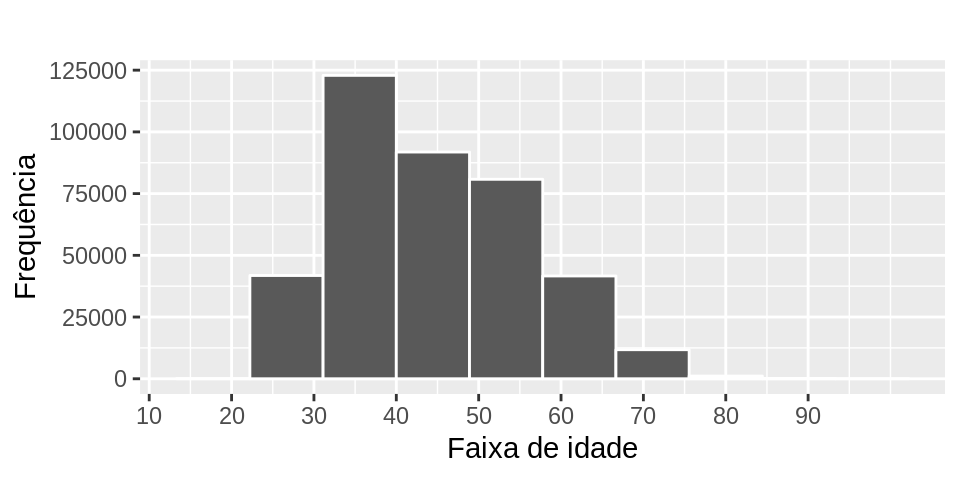
\includegraphics{ebookrnp_files/figure-latex/graf08-1} 

}

\caption{Histograma idade do docente}\label{fig:graf08}
\end{figure}

Veja que a figura \ref{fig:graf08} evidencia que as maiores concetrações de docentes estão nas faixas de idade entre 30 e 50 anos.

\hypertarget{densidade}{%
\subsubsection{Densidade}\label{densidade}}

Gráficos de densidade possuem aplicação semelhante aos hitogramas, porém são mais indicados pata amostras grandes. Ele evidenciam a melhor curva que representam os dados. Este tipo de gráfico nos ajuda também a verificar a distribuição de probabilidade aproximada que os dados podem seguir.

\BeginKnitrBlock{example}
\protect\hypertarget{exm:unnamed-chunk-56}{}{\label{exm:unnamed-chunk-56} }Vamos criar agora um gráfico de densidade para a variável idade dos docentes.
\EndKnitrBlock{example}

\begin{Shaded}
\begin{Highlighting}[]
\NormalTok{p <-}\StringTok{ }\NormalTok{ggplot2}\OperatorTok{::}\KeywordTok{ggplot}\NormalTok{(base_docentes, }\KeywordTok{aes}\NormalTok{(}\DataTypeTok{x =}\NormalTok{ idade))}
\NormalTok{p }\OperatorTok{+}\StringTok{ }\NormalTok{ggplot2}\OperatorTok{::}\KeywordTok{theme_gray}\NormalTok{() }\OperatorTok{+}
\StringTok{  }\NormalTok{ggplot2}\OperatorTok{::}\KeywordTok{geom_density}\NormalTok{(}\DataTypeTok{adjust =} \DecValTok{1}\NormalTok{) }\OperatorTok{+}
\StringTok{  }\NormalTok{ggplot2}\OperatorTok{::}\KeywordTok{labs}\NormalTok{(}\DataTypeTok{y =} \StringTok{"Densidade"}\NormalTok{, }\DataTypeTok{x =} \StringTok{"Idade"}\NormalTok{, }\DataTypeTok{fill =} \OtherTok{NULL}\NormalTok{, }\DataTypeTok{title =} \StringTok{""}\NormalTok{) }\OperatorTok{+}
\StringTok{  }\NormalTok{ggplot2}\OperatorTok{::}\KeywordTok{scale_x_continuous}\NormalTok{(}
    \DataTypeTok{breaks=}\KeywordTok{seq}\NormalTok{(}\DecValTok{10}\NormalTok{, }\DecValTok{90}\NormalTok{, }\DecValTok{10}\NormalTok{),}
    \DataTypeTok{labels =} \KeywordTok{seq}\NormalTok{(}\DecValTok{10}\NormalTok{, }\DecValTok{90}\NormalTok{, }\DecValTok{10}\NormalTok{)) }\OperatorTok{+}
\StringTok{  }\NormalTok{ggplot2}\OperatorTok{::}\KeywordTok{theme}\NormalTok{(}\DataTypeTok{axis.line =} \KeywordTok{element_blank}\NormalTok{())}
\end{Highlighting}
\end{Shaded}

\begin{figure}[H]

{\centering 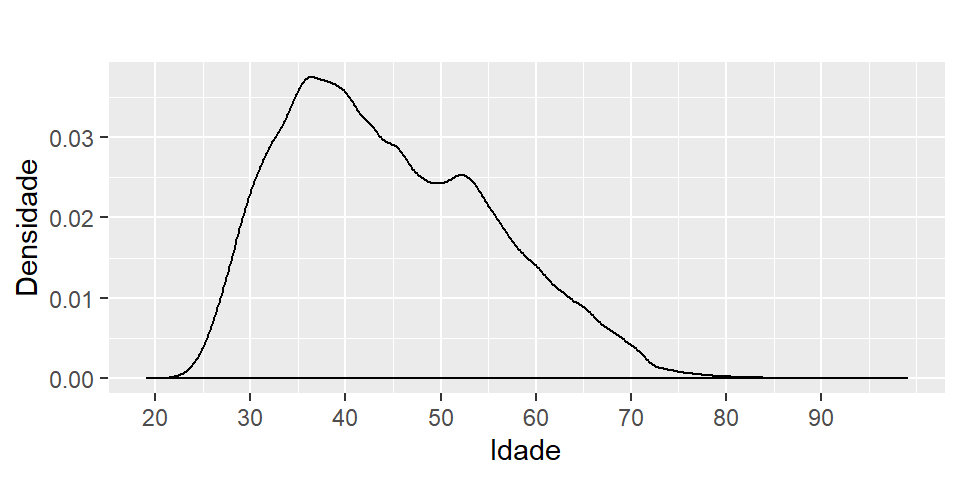
\includegraphics{ebookrnp_files/figure-latex/graf09-1} 

}

\caption{Densidade idade do docente}\label{fig:graf09}
\end{figure}

Perceba na figura \ref{fig:graf08} como esperado, que a densidade dos dados está concentrada idade entre 30 e 50 anos. Porém, ela aponta uma elevação próxima a 50 anos apontando comportamento bimodal nos dados.

\hypertarget{box-plot}{%
\subsubsection{Box-Plot}\label{box-plot}}

De longe o gráfico Box-plot ou para muitos, diagrama de caixa é o tipo mais completo de gráfico para variável numérica.

\begin{figure}[H]

{\centering 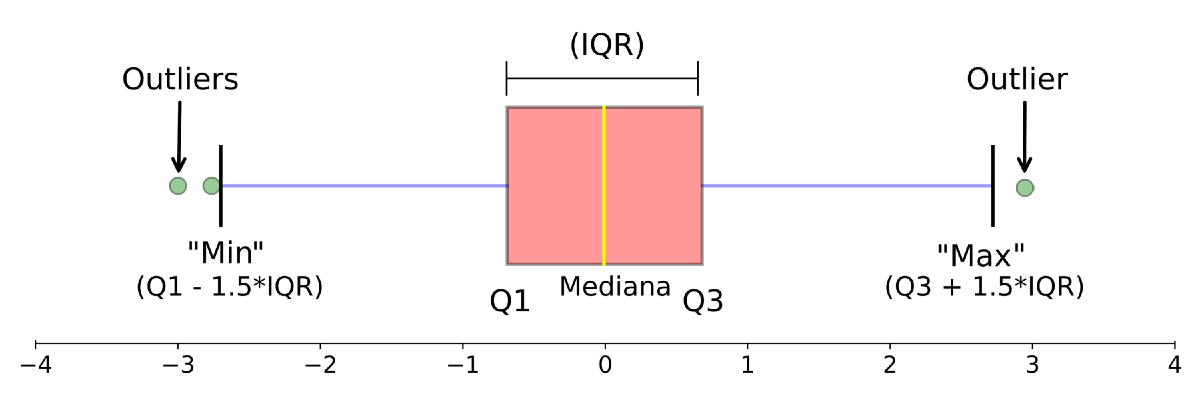
\includegraphics[width=1\linewidth]{../Imagens/ebook_boxplot} 

}

\caption{Definindo um Box-plot}\label{fig:fig10}
\end{figure}

A figura \ref{fig:fig10} ilustra os elementos que compõem um Box-plot. Perceba que visualmente ele contempla as estatísticas \(Q_1\), \(Q_2\) (mediana), \(Q_3, IQR, LI,LS\) e \emph{outliers}. Com base nestas estatísticas, uma variável numéricas estará bem caracterizada.

\BeginKnitrBlock{example}
\protect\hypertarget{exm:unnamed-chunk-57}{}{\label{exm:unnamed-chunk-57} }Ainda para os dados de idade, vamos montar um Box-plot
\EndKnitrBlock{example}

\begin{Shaded}
\begin{Highlighting}[]
\NormalTok{p <-}\StringTok{ }\NormalTok{ggplot2}\OperatorTok{::}\KeywordTok{ggplot}\NormalTok{(base_docentes, }\KeywordTok{aes}\NormalTok{(}\DataTypeTok{y =}\NormalTok{ idade))}
\NormalTok{p }\OperatorTok{+}\StringTok{ }\NormalTok{ggplot2}\OperatorTok{::}\KeywordTok{theme_gray}\NormalTok{() }\OperatorTok{+}
\StringTok{  }\NormalTok{ggplot2}\OperatorTok{::}\KeywordTok{geom_boxplot}\NormalTok{(}\DataTypeTok{adjust =} \DecValTok{1}\NormalTok{) }\OperatorTok{+}
\StringTok{  }\NormalTok{ggplot2}\OperatorTok{::}\KeywordTok{labs}\NormalTok{(}\DataTypeTok{x =} \StringTok{""}\NormalTok{, }\DataTypeTok{y =} \StringTok{"Idade"}\NormalTok{, }\DataTypeTok{fill =} \OtherTok{NULL}\NormalTok{, }\DataTypeTok{title =} \StringTok{""}\NormalTok{) }\OperatorTok{+}
\StringTok{  }\NormalTok{ggplot2}\OperatorTok{::}\KeywordTok{coord_flip}\NormalTok{() }\OperatorTok{+}
\StringTok{  }\NormalTok{ggplot2}\OperatorTok{::}\KeywordTok{theme}\NormalTok{(}\DataTypeTok{axis.line.x =} \KeywordTok{element_line}\NormalTok{(), }
                 \DataTypeTok{axis.text.x =} \OtherTok{NULL}\NormalTok{, }
                 \DataTypeTok{axis.line.y =} \KeywordTok{element_blank}\NormalTok{())}
\end{Highlighting}
\end{Shaded}

\begin{figure}[H]

{\centering 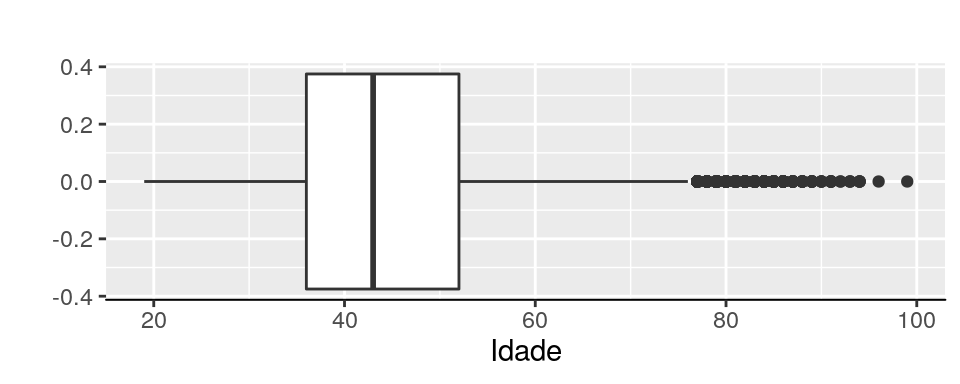
\includegraphics{ebookrnp_files/figure-latex/graf11-1} 

}

\caption{Box-plot idade do docente}\label{fig:graf11}
\end{figure}

Conforme vimos antes, idades acima de 76 anos são pontos atípicos na base de docentes, por isso no Box-plot estes pontos aparecem fora do limite superior de outliers na figura \ref{fig:fig11}.

\hypertarget{graficos-para-duas-variaveis-numericas}{%
\subsection{Gráficos para duas variáveis numéricas}\label{graficos-para-duas-variaveis-numericas}}

Os principais gráficos para analisar a relação entre duas variáveis são o gráfico de pontos ou \emph{scatterplot} e o gráfico de linhas, através deles é possível analisar a relação conjunta entre as variáveis e determinar se uma influencia a outra de alguma forma. além destes, também podemos traçar gráficos de densidade para comparar as duas curvas.

\hypertarget{scatterplot}{%
\subsubsection{\texorpdfstring{\emph{scatterplot}}{scatterplot}}\label{scatterplot}}

O gráfico de pontos é um gráfico bidimensional onde cada eixo representa os valores de uma variável. Este tipo de gráfico é ótimo para analisar a correlação de duas variáveis bem como sua dispersão, pois cada ponto representa a ligação dos elementos das duas variáveis.

\BeginKnitrBlock{example}
\protect\hypertarget{exm:unnamed-chunk-58}{}{\label{exm:unnamed-chunk-58} }Para lustrar vamos traçar um gráfico de pontos para a receita próprias das IES pelo total de técnicos na base das IES.
Obs.: como temos muitos autliers na variável de receita própria, vamos limitar a 10.000.000 (dez milhões de reais por ano)
\EndKnitrBlock{example}

\begin{Shaded}
\begin{Highlighting}[]
\NormalTok{p <-}\StringTok{ }\NormalTok{base_ies }\OperatorTok\StringTok{ }
\StringTok{  }\NormalTok{dplyr}\OperatorTok{::}\KeywordTok{filter}\NormalTok{(ReceitaPropria }\OperatorTok{<=}\StringTok{ }\DecValTok{10000000}\NormalTok{) }\OperatorTok\StringTok{ }
\StringTok{  }\NormalTok{ggplot2}\OperatorTok{::}\KeywordTok{ggplot}\NormalTok{(}\KeywordTok{aes}\NormalTok{(}\DataTypeTok{x =}\NormalTok{ TotalTecnicos, }\DataTypeTok{y =}\NormalTok{ ReceitaPropria))}
\NormalTok{p }\OperatorTok{+}\StringTok{ }\NormalTok{ggplot2}\OperatorTok{::}\KeywordTok{theme_gray}\NormalTok{() }\OperatorTok{+}
\StringTok{  }\NormalTok{ggplot2}\OperatorTok{::}\KeywordTok{geom_point}\NormalTok{() }\OperatorTok{+}
\StringTok{  }\NormalTok{ggplot2}\OperatorTok{::}\KeywordTok{labs}\NormalTok{(}\DataTypeTok{x =} \StringTok{"Total técnicos"}\NormalTok{, }\DataTypeTok{y =} \StringTok{"Receita própria", fill = NULL, title = "") +}
\StringTok{  ggplot2::theme(axis.line.x = element_line(), }
\StringTok{                 axis.text.x = NULL, }
\StringTok{                 axis.line.y = element_blank())}
\end{Highlighting}
\end{Shaded}

\begin{figure}[H]

{\centering 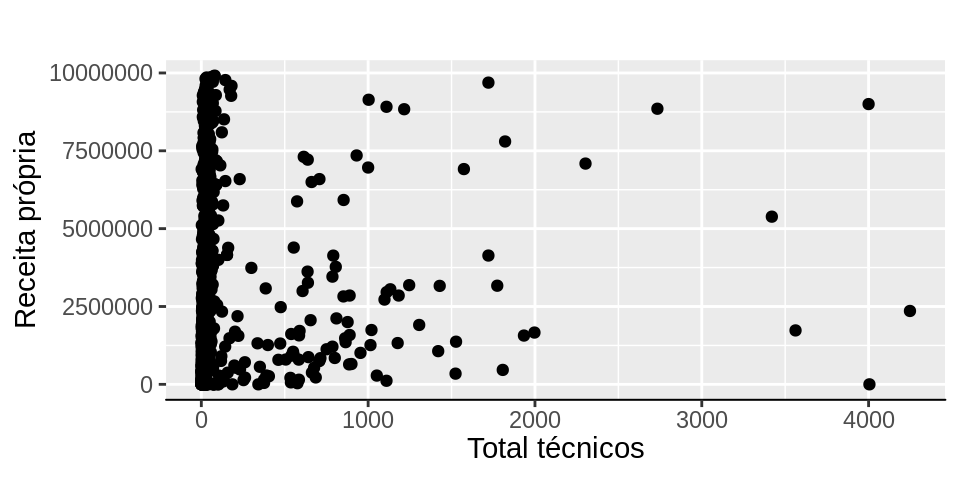
\includegraphics{ebookrnp_files/figure-latex/graf12-1} 

}

\caption{Gráfico de pontos total de técnicos versus receita própria}\label{fig:graf12}
\end{figure}

\hypertarget{grafico-de-linhas}{%
\subsubsection{Grafico de linhas}\label{grafico-de-linhas}}

O gráfico de linhas possui aplicação para duas variáveis contínuas e também para séries temporais, onde um dos eixos é uma variável numerica de data.

\begin{Shaded}
\begin{Highlighting}[]
\NormalTok{p <-}\StringTok{ }\NormalTok{base_ies }\OperatorTok\StringTok{ }
\StringTok{  }\NormalTok{dplyr}\OperatorTok{::}\KeywordTok{filter}\NormalTok{(TotalTecnicos }\OperatorTok{<}\StringTok{ }\DecValTok{100}\NormalTok{) }\OperatorTok\StringTok{ }
\StringTok{  }\NormalTok{ggplot2}\OperatorTok{::}\KeywordTok{ggplot}\NormalTok{(}\KeywordTok{aes}\NormalTok{(}\DataTypeTok{x =}\NormalTok{ TotalTecnicos, }\DataTypeTok{y =}\NormalTok{ ReceitaPropria))}
\NormalTok{p }\OperatorTok{+}\StringTok{ }\NormalTok{ggplot2}\OperatorTok{::}\KeywordTok{theme_gray}\NormalTok{() }\OperatorTok{+}
\StringTok{  }\NormalTok{ggplot2}\OperatorTok{::}\KeywordTok{geom_line}\NormalTok{() }\OperatorTok{+}
\StringTok{  }\NormalTok{ggplot2}\OperatorTok{::}\KeywordTok{labs}\NormalTok{(}\DataTypeTok{x =} \StringTok{"Total técnicos"}\NormalTok{, }\DataTypeTok{y =} \StringTok{"Receita própria", }
\StringTok{                fill = NULL, title = "") +}
\StringTok{  ggplot2::theme(axis.line.x = element_line(), }
\StringTok{                 axis.text.x = NULL, }
\StringTok{                 axis.line.y = element_blank())}
\end{Highlighting}
\end{Shaded}

\begin{figure}[H]

{\centering 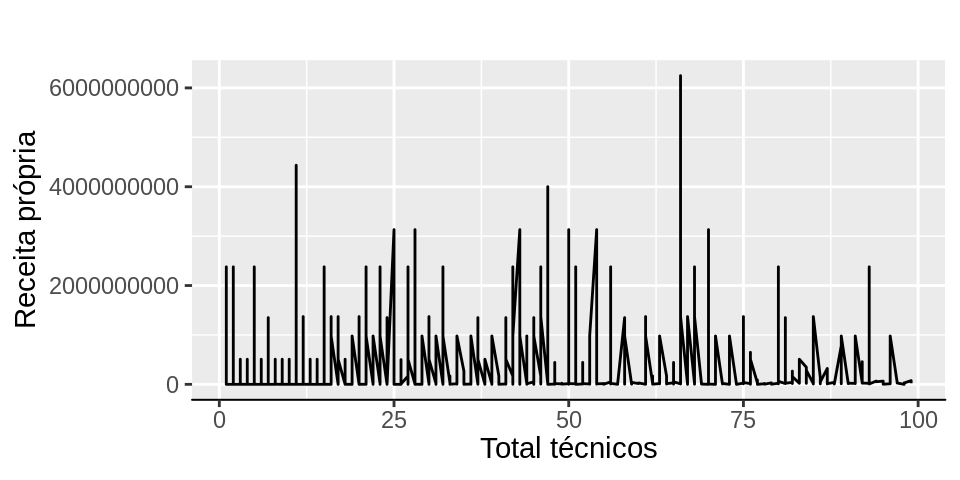
\includegraphics{ebookrnp_files/figure-latex/graf13-1} 

}

\caption{Gráfico de pontos total de técnicos (<50) versus receita própria}\label{fig:graf13}
\end{figure}

\hypertarget{variaveis-categoricas-versus-numericas}{%
\section{Variáveis categóricas versus numéricas}\label{variaveis-categoricas-versus-numericas}}

O trabalho estatístico muitas vezes exige que alguma variável numérica seja categorizada ou analisada em conjunto com alguma variável categórica. Todas as técnicas vistas até agora, tanto as medidas estatísticas quanto os gráficos podem ser analisados em conjunto para gerar informação.

\hypertarget{categorizando-variaveis-numericas.}{%
\subsection{Categorizando variáveis numéricas.}\label{categorizando-variaveis-numericas.}}

Em R podemos agrupar uma variável numérica de muitas formas, umas delas é através das estatísticas de quartis, decis ou percentis dependendo do tamanho da base, com a função \texttt{quantile()} combinada com a função \texttt{cut()}. Outra forma é através do conhecimento próprio do analista com os operadores relacionais do R: \texttt{\textless{},\ \textgreater{},\ \textgreater{}=,\ \textless{}=,\ ==,\ !=,\ \%in\%} combinadas com \texttt{ifelse()}.

\BeginKnitrBlock{example}
\protect\hypertarget{exm:unnamed-chunk-59}{}{\label{exm:unnamed-chunk-59} }Vamos categorizar a variável receita próprias das IES de duas formas distintas: por quartis e por operadores relacionais com quatro faixas.
\EndKnitrBlock{example}

\begin{Shaded}
\begin{Highlighting}[]
\NormalTok{## Categorizando por quartis}
\NormalTok{fx_receita_q <-}\StringTok{ }\KeywordTok{cut}\NormalTok{(base_ies}\OperatorTok{$}\NormalTok{ReceitaPropria, }
                   \DataTypeTok{breaks =} \KeywordTok{round}\NormalTok{(}\KeywordTok{quantile}\NormalTok{(base_ies}\OperatorTok{$}\NormalTok{ReceitaPropria)), }
                   \DataTypeTok{dig.lab =} \DecValTok{10}\NormalTok{, }\DataTypeTok{include.lowest =} \OtherTok{TRUE}\NormalTok{)}
\NormalTok{rnp}\OperatorTok{::}\KeywordTok{rnp_freq}\NormalTok{(fx_receita_q, }\DataTypeTok{sortd =} \OtherTok{FALSE}\NormalTok{) }\OperatorTok\StringTok{ }
\NormalTok{knitr}\OperatorTok{::}\KeywordTok{kable}\NormalTok{(}\DataTypeTok{digits =} \DecValTok{3}\NormalTok{,}
             \DataTypeTok{booktabs =} \OtherTok{TRUE}\NormalTok{, }\DataTypeTok{format =}\NormalTok{ tb_formata,}
             \DataTypeTok{caption =} \StringTok{"Categorização por quartis"}\NormalTok{) }\OperatorTok\StringTok{ }
\NormalTok{kableExtra}\OperatorTok{::}\KeywordTok{kable_styling}\NormalTok{(}\DataTypeTok{latex_options =} \StringTok{"hold_position"}\NormalTok{)}
\end{Highlighting}
\end{Shaded}

\begin{table}[!h]

\caption{\label{tab:tab09}Categorização por quartis}
\centering
\begin{tabular}{lrrrr}
\toprule
classe & fa & fr & Faa & Fra\\
\midrule
0--1389966 & 612 & 0.25 & 612 & 0.25\\
1389966--7429221 & 612 & 0.25 & 1224 & 0.50\\
7429221--61258594 & 612 & 0.25 & 1836 & 0.75\\
61258594--6248050290 & 612 & 0.25 & 2448 & 1.00\\
\bottomrule
\end{tabular}
\end{table}

\begin{Shaded}
\begin{Highlighting}[]
\NormalTok{## Categorização por ifelse com operadores relacionais}
\NormalTok{fx_receita_r <-}\StringTok{ }\KeywordTok{ifelse}\NormalTok{(base_ies}\OperatorTok{$}\NormalTok{ReceitaPropria }\OperatorTok{<=}\StringTok{ }\DecValTok{1200000}\NormalTok{, }\StringTok{"A.-1200000"}\NormalTok{,}
                \KeywordTok{ifelse}\NormalTok{(base_ies}\OperatorTok{$}\NormalTok{ReceitaPropria }\OperatorTok{<=}\StringTok{ }\DecValTok{5000000}\NormalTok{, }\StringTok{"B.1200000 a 5000000"}\NormalTok{,}
                \KeywordTok{ifelse}\NormalTok{(base_ies}\OperatorTok{$}\NormalTok{ReceitaPropria }\OperatorTok{<=}\DecValTok{35000000}\NormalTok{, }\StringTok{"C.5000000 a 35000000"}\NormalTok{,}\StringTok{"D.35000000+"}\NormalTok{)))}

\NormalTok{rnp}\OperatorTok{::}\KeywordTok{rnp_freq}\NormalTok{(fx_receita_r, }\DataTypeTok{sortd =} \OtherTok{FALSE}\NormalTok{) }\OperatorTok\StringTok{ }
\NormalTok{knitr}\OperatorTok{::}\KeywordTok{kable}\NormalTok{(}\DataTypeTok{digits =} \DecValTok{3}\NormalTok{,}
             \DataTypeTok{booktabs =} \OtherTok{TRUE}\NormalTok{, }\DataTypeTok{format =}\NormalTok{ tb_formata,}
             \DataTypeTok{caption =} \StringTok{"Categorização por operadores relacionais"}\NormalTok{) }\OperatorTok\StringTok{ }
\NormalTok{kableExtra}\OperatorTok{::}\KeywordTok{kable_styling}\NormalTok{(}\DataTypeTok{latex_options =} \StringTok{"hold_position"}\NormalTok{)}
\end{Highlighting}
\end{Shaded}

\begin{table}[!h]

\caption{\label{tab:tab09}Categorização por operadores relacionais}
\centering
\begin{tabular}{lrrrr}
\toprule
classe & fa & fr & Faa & Fra\\
\midrule
A.-1200000 & 571 & 0.233 & 571 & 0.233\\
B.1200000 a 5000000 & 500 & 0.204 & 1071 & 0.438\\
C.5000000 a 35000000 & 635 & 0.259 & 1706 & 0.697\\
D.35000000+ & 742 & 0.303 & 2448 & 1.000\\
\bottomrule
\end{tabular}
\end{table}

No primeiro caso, criamos os cortes utilizando os quartis da variável e em seguida passamos estes cortes para a função \texttt{cut()} que por sua vez particionou a variável de acor com as partes informadas pelo argumento \texttt{breaks}. Desta forma fica mais rapido a categorização, mas o analista não tem como persolaizar as faixas. Para atender a esta limitação o segundo método ajuda a customizar as faixas de acordo com a preferência ou necessidade. Embora exija um pouco mais de código, esta última opção é mais flexível.

\hypertarget{medidas-estatisticas-por-agrupamento}{%
\subsection{Medidas estatísticas por agrupamento}\label{medidas-estatisticas-por-agrupamento}}

Em muitas situações da análise de dados, estamos interessados em analisar a influência de uma variável categórica sob uma ou mais variáveis numéricas. Felizmente, a grande maioria das medidas estatísticas aprendidas até agora se aplicam a este tipo de análise que exige estatísticas agrupadas.

\BeginKnitrBlock{example}
\protect\hypertarget{exm:unnamed-chunk-60}{}{\label{exm:unnamed-chunk-60} }Vamos calcular estatísticas descritivas de idade dos docentes (em anos) por escolaridade.
\EndKnitrBlock{example}

\begin{Shaded}
\begin{Highlighting}[]
\NormalTok{base_docentes }\OperatorTok\StringTok{ }
\StringTok{  }\NormalTok{dplyr}\OperatorTok{::}\KeywordTok{group_by}\NormalTok{(escolaridade) }\OperatorTok\StringTok{ }
\StringTok{  }\NormalTok{dplyr}\OperatorTok{::}\KeywordTok{summarise}\NormalTok{(}\DataTypeTok{N    =} \KeywordTok{n}\NormalTok{(),}
                   \DataTypeTok{Min  =} \KeywordTok{min}\NormalTok{(idade),}
                   \DataTypeTok{Q1   =} \KeywordTok{unname}\NormalTok{(}\KeywordTok{quantile}\NormalTok{(idade, }\DataTypeTok{probs =} \FloatTok{0.25}\NormalTok{)),}
                   \DataTypeTok{Me   =} \KeywordTok{mean}\NormalTok{(idade),}
                   \DataTypeTok{Md   =} \KeywordTok{median}\NormalTok{(idade),}
                   \DataTypeTok{Q3   =} \KeywordTok{unname}\NormalTok{(}\KeywordTok{quantile}\NormalTok{(idade, }\DataTypeTok{probs =} \FloatTok{0.75}\NormalTok{)),}
                   \DataTypeTok{Max  =} \KeywordTok{max}\NormalTok{(idade)}
                   \CommentTok{#Dp   = sd(idade),}
                   \CommentTok{#cv   = sd(idade)/mean(idade)}
\NormalTok{                   ) }\OperatorTok\StringTok{ }
\StringTok{  }\NormalTok{knitr}\OperatorTok{::}\KeywordTok{kable}\NormalTok{(}\DataTypeTok{digits =} \DecValTok{2}\NormalTok{,}
             \DataTypeTok{booktabs =} \OtherTok{TRUE}\NormalTok{, }\DataTypeTok{format =}\NormalTok{ tb_formata,}
             \DataTypeTok{caption =} \StringTok{"Estatísticas descritivas idade vs escolaridade"}\NormalTok{) }\OperatorTok\StringTok{ }
\NormalTok{kableExtra}\OperatorTok{::}\KeywordTok{kable_styling}\NormalTok{(}\DataTypeTok{latex_options =} \StringTok{"hold_position"}\NormalTok{)}
\end{Highlighting}
\end{Shaded}

\begin{table}[!h]

\caption{\label{tab:tab11}Estatísticas descritivas idade vs escolaridade}
\centering
\begin{tabular}{lrrrrrrr}
\toprule
escolaridade & N & Min & Q1 & Me & Md & Q3 & Max\\
\midrule
1. Sem graduação & 10 & 23 & 47.25 & 52.60 & 54 & 63 & 66\\
2. Graduação & 4613 & 20 & 27.00 & 37.78 & 33 & 45 & 94\\
3. Especialização & 72301 & 19 & 35.00 & 43.01 & 41 & 50 & 93\\
4. Mestrado & 154285 & 22 & 34.00 & 42.81 & 41 & 50 & 90\\
5. Doutorado & 160827 & 19 & 38.00 & 47.06 & 46 & 54 & 99\\
\bottomrule
\end{tabular}
\end{table}

Em \(Q3\) temos que 75\% dos docentes com Doutorado possuem idade até 54 anos. Vemos também alguns doutores excepcionais com idade mínima de 19 anos. A idade máxima registrada foi de 99 anos presente no grupos dos doutores. A categoria sem graduação tem dez indivíduos e é pouco representativa.

\begin{Shaded}
\begin{Highlighting}[]
\CommentTok{# Como nossa rnp_summary, poderiamos fazer assim}
\KeywordTok{aggregate}\NormalTok{(idade }\OperatorTok{~}\StringTok{ }\NormalTok{escolaridade,}
          \DataTypeTok{data =}\NormalTok{ base_docentes,}
          \DataTypeTok{FUN =} \ControlFlowTok{function}\NormalTok{(i) rnp}\OperatorTok{::}\KeywordTok{rnp_summary}\NormalTok{(i))}
\end{Highlighting}
\end{Shaded}

\hypertarget{graficos-para-categoricas-vs-numericas}{%
\subsection{Gráficos para categóricas vs numéricas}\label{graficos-para-categoricas-vs-numericas}}

Com apoio do pacote \texttt{ggplot} podemos combinar a maioria dos gráficos vistos até agora para analisar dados por grupo ou classes. Como citamos na seção 1.6 uma das ferramentas estatísticas é a análise bivariada e ela pode ser feita entre duas variáveis podendo ser de mesmo tipo ou de tipos diferentes

\begin{itemize}
\tightlist
\item
  \textbf{Box-plot agrupado}: Box-plots por cateoria são muito informativos uma vez que resumem sete estatísticas fudnamentais de uma variável continua conforma já vimos.
\end{itemize}

\BeginKnitrBlock{example}
\protect\hypertarget{exm:unnamed-chunk-62}{}{\label{exm:unnamed-chunk-62} }Represente visualmente a análise da tabela \ref{tab:tab11} através de Box-plots.
\EndKnitrBlock{example}

\begin{Shaded}
\begin{Highlighting}[]
\NormalTok{p <-}\StringTok{ }\NormalTok{base_docentes }\OperatorTok\StringTok{ }
\StringTok{  }\NormalTok{ggplot2}\OperatorTok{::}\KeywordTok{ggplot}\NormalTok{(}\KeywordTok{aes}\NormalTok{(}\DataTypeTok{x =}\NormalTok{ escolaridade, }\DataTypeTok{y =}\NormalTok{ idade, }\DataTypeTok{fill =}\NormalTok{ escolaridade))}
\NormalTok{p }\OperatorTok{+}\StringTok{ }\NormalTok{ggplot2}\OperatorTok{::}\KeywordTok{theme_gray}\NormalTok{() }\OperatorTok{+}
\StringTok{  }\NormalTok{ggplot2}\OperatorTok{::}\KeywordTok{geom_boxplot}\NormalTok{(}\DataTypeTok{show.legend =} \OtherTok{FALSE}\NormalTok{) }\OperatorTok{+}
\StringTok{  }\NormalTok{ggplot2}\OperatorTok{::}\KeywordTok{coord_flip}\NormalTok{()}\OperatorTok{+}
\StringTok{  }\NormalTok{ggplot2}\OperatorTok{::}\KeywordTok{theme}\NormalTok{(}\DataTypeTok{axis.line.x =} \KeywordTok{element_line}\NormalTok{(), }
                 \DataTypeTok{axis.text.x =} \OtherTok{NULL}\NormalTok{, }
                 \DataTypeTok{axis.line.y =} \KeywordTok{element_blank}\NormalTok{())}
\end{Highlighting}
\end{Shaded}

\begin{figure}[H]

{\centering 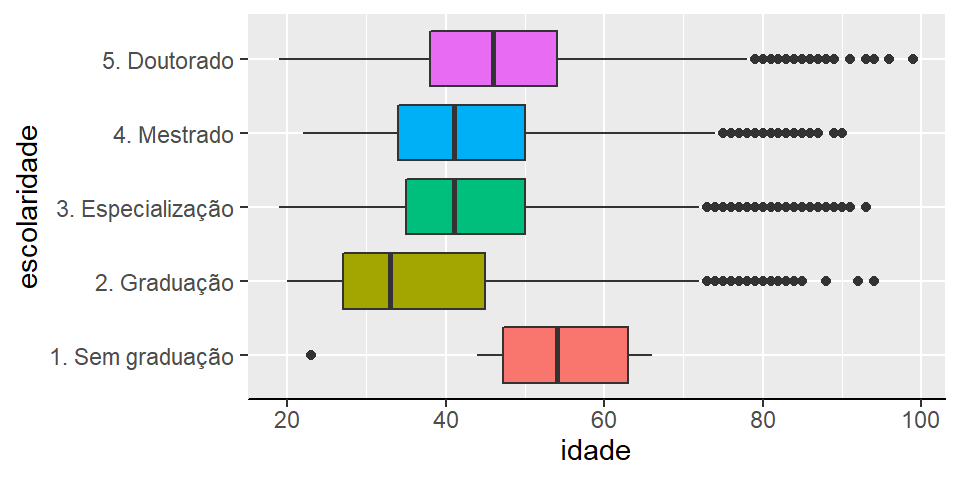
\includegraphics{ebookrnp_files/figure-latex/graf14-1} 

}

\caption{Box-plot de idade vs escolaridade}\label{fig:graf14}
\end{figure}

No Box-plot conseguimos ver que docentes com graduação apenas são minoria como visto na tabela e doutores são maioria. Notamos também que, com exceção daqueles sem graduação todos os grupos possuem dispersão pareceida uma vez que adistância entre \(Q_1\) e \(Q_3\) é pequena.

\begin{quote}
Para todos os graficos agrupados também é possível quebrar a visualização em um gráfico por categoria adicionando uma terceira variável com facet\_wrap() .
\end{quote}

\begin{Shaded}
\begin{Highlighting}[]
\NormalTok{p <-}\StringTok{ }\NormalTok{base_docentes }\OperatorTok\StringTok{ }
\StringTok{  }\NormalTok{ggplot2}\OperatorTok{::}\KeywordTok{ggplot}\NormalTok{(}\KeywordTok{aes}\NormalTok{(}\DataTypeTok{x =}\NormalTok{ sexo, }\DataTypeTok{y =}\NormalTok{ idade, }\DataTypeTok{fill =}\NormalTok{ escolaridade))}
\NormalTok{p }\OperatorTok{+}\StringTok{ }\NormalTok{ggplot2}\OperatorTok{::}\KeywordTok{theme_gray}\NormalTok{() }\OperatorTok{+}
\StringTok{  }\NormalTok{ggplot2}\OperatorTok{::}\KeywordTok{geom_boxplot}\NormalTok{(}\DataTypeTok{show.legend =} \OtherTok{FALSE}\NormalTok{) }\OperatorTok{+}
\StringTok{  }\NormalTok{ggplot2}\OperatorTok{::}\KeywordTok{coord_flip}\NormalTok{()}\OperatorTok{+}
\StringTok{  }\NormalTok{ggplot2}\OperatorTok{::}\KeywordTok{facet_wrap}\NormalTok{(escolaridade}\OperatorTok{~}\NormalTok{.)}\OperatorTok{+}
\StringTok{  }\NormalTok{ggplot2}\OperatorTok{::}\KeywordTok{theme}\NormalTok{(}\DataTypeTok{axis.line.x =} \KeywordTok{element_line}\NormalTok{(), }
                 \DataTypeTok{axis.text.x =} \OtherTok{NULL}\NormalTok{, }
                 \DataTypeTok{axis.line.y =} \KeywordTok{element_blank}\NormalTok{())}
\end{Highlighting}
\end{Shaded}

\begin{figure}[H]

{\centering 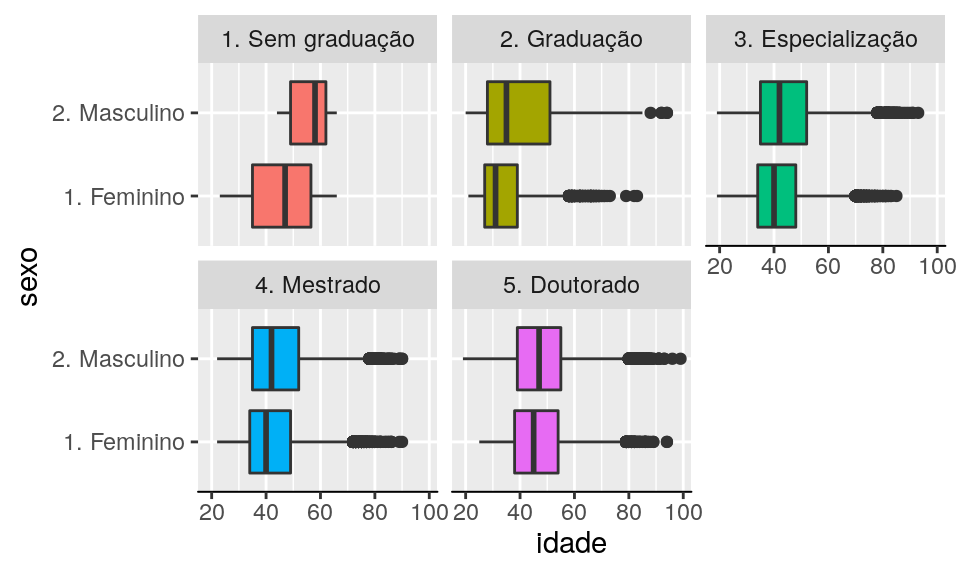
\includegraphics{ebookrnp_files/figure-latex/unnamed-chunk-63-1} 

}

\caption{Box-plot de idade vs escolaridade por sexo}\label{fig:unnamed-chunk-63}
\end{figure}

\begin{itemize}
\tightlist
\item
  \textbf{Gráfico de densidade agrupado}: é possível comparara várias curvas simultaneamente no mesmo gráfico para analisar a distribuição dos dados.
\end{itemize}

\BeginKnitrBlock{example}
\protect\hypertarget{exm:unnamed-chunk-64}{}{\label{exm:unnamed-chunk-64} }Represente visualmente a análise da tabela \ref{tab:tab11} desta vez utilizando \emph{densityplot}.
\EndKnitrBlock{example}

\begin{Shaded}
\begin{Highlighting}[]
\NormalTok{p <-}\StringTok{ }\NormalTok{base_docentes }\OperatorTok\StringTok{ }
\StringTok{  }\NormalTok{ggplot2}\OperatorTok{::}\KeywordTok{ggplot}\NormalTok{(}\KeywordTok{aes}\NormalTok{(}\DataTypeTok{x =}\NormalTok{ idade, }\DataTypeTok{fill =}\NormalTok{ escolaridade))}
\NormalTok{p }\OperatorTok{+}\StringTok{ }\NormalTok{ggplot2}\OperatorTok{::}\KeywordTok{theme_gray}\NormalTok{() }\OperatorTok{+}
\StringTok{  }\NormalTok{ggplot2}\OperatorTok{::}\KeywordTok{geom_density}\NormalTok{(}\DataTypeTok{alpha =} \FloatTok{0.6}\NormalTok{) }\OperatorTok{+}
\StringTok{  }\NormalTok{ggplot2}\OperatorTok{::}\KeywordTok{theme}\NormalTok{(}\DataTypeTok{legend.position =} \StringTok{"right"}\NormalTok{) }\OperatorTok{+}
\StringTok{  }\NormalTok{ggplot2}\OperatorTok{::}\KeywordTok{theme}\NormalTok{(}\DataTypeTok{axis.line.x =} \KeywordTok{element_line}\NormalTok{(), }
                 \DataTypeTok{axis.text.x =} \OtherTok{NULL}\NormalTok{, }\DataTypeTok{axis.line.y =} \KeywordTok{element_blank}\NormalTok{()) }\OperatorTok{+}
\StringTok{  }\NormalTok{ggplot2}\OperatorTok{::}\KeywordTok{labs}\NormalTok{(}\DataTypeTok{x =} \StringTok{"Idade"}\NormalTok{, }\DataTypeTok{y =} \StringTok{"Densidade"}\NormalTok{, }\DataTypeTok{fill =} \OtherTok{NULL}\NormalTok{, }\DataTypeTok{title =} \StringTok{""}\NormalTok{)}
\end{Highlighting}
\end{Shaded}

\begin{figure}[H]

{\centering 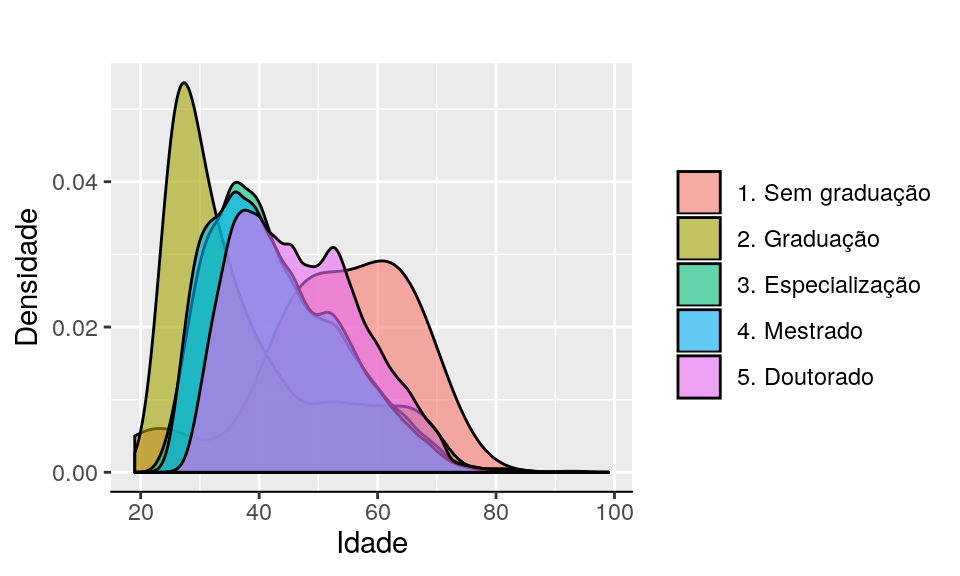
\includegraphics{ebookrnp_files/figure-latex/graf15-1} 

}

\caption{Densidade de idade vs escolaridade}\label{fig:graf15}
\end{figure}

O resultado é um gráfico elegante e que indica precisamente a forma da distribuição dos dados.

Agora quebrado por sexo.

\begin{Shaded}
\begin{Highlighting}[]
\NormalTok{p <-}\StringTok{ }\NormalTok{base_docentes }\OperatorTok\StringTok{ }
\StringTok{  }\NormalTok{ggplot2}\OperatorTok{::}\KeywordTok{ggplot}\NormalTok{(}\KeywordTok{aes}\NormalTok{(}\DataTypeTok{x =}\NormalTok{ idade, }\DataTypeTok{color =}\NormalTok{ sexo, }\DataTypeTok{fill =}\NormalTok{ escolaridade))}
\NormalTok{p }\OperatorTok{+}\StringTok{ }\NormalTok{ggplot2}\OperatorTok{::}\KeywordTok{theme_gray}\NormalTok{() }\OperatorTok{+}
\StringTok{  }\NormalTok{ggplot2}\OperatorTok{::}\KeywordTok{geom_density}\NormalTok{(}\DataTypeTok{alpha =} \FloatTok{0.6}\NormalTok{, }\DataTypeTok{show.legend =} \OtherTok{FALSE}\NormalTok{) }\OperatorTok{+}
\StringTok{  }\NormalTok{ggplot2}\OperatorTok{::}\KeywordTok{facet_wrap}\NormalTok{(}\OperatorTok{~}\NormalTok{escolaridade)}\OperatorTok{+}
\StringTok{  }\NormalTok{ggplot2}\OperatorTok{::}\KeywordTok{theme}\NormalTok{(}\DataTypeTok{axis.line.x =} \KeywordTok{element_line}\NormalTok{(), }
                 \DataTypeTok{axis.text.x =} \OtherTok{NULL}\NormalTok{, }
                 \DataTypeTok{axis.line.y =} \KeywordTok{element_blank}\NormalTok{()) }\OperatorTok{+}
\StringTok{  }\NormalTok{ggplot2}\OperatorTok{::}\KeywordTok{labs}\NormalTok{(}\DataTypeTok{x =} \StringTok{"Idade"}\NormalTok{, }\DataTypeTok{y =} \StringTok{"Densidade"}\NormalTok{, }\DataTypeTok{fill =} \OtherTok{NULL}\NormalTok{, }\DataTypeTok{title =} \StringTok{""}\NormalTok{)}
\end{Highlighting}
\end{Shaded}

\begin{figure}[H]

{\centering 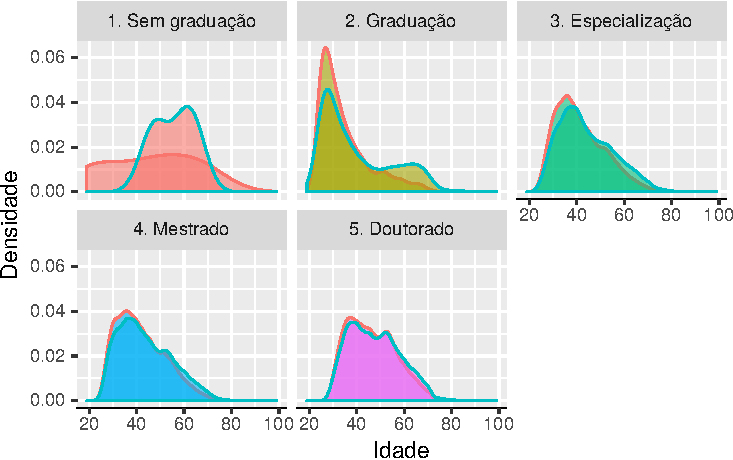
\includegraphics{ebookrnp_files/figure-latex/unnamed-chunk-65-1} 

}

\caption{Densidade de idade vs escolaridade por sexo}\label{fig:unnamed-chunk-65}
\end{figure}

\begin{itemize}
\tightlist
\item
  \textbf{Gráfico de colunas agrupadas}: é possível assim, como nos dois últimos exmeplos, gerar gráficos e coluna agrupadas e fazer a quebra adiconando uma terceira variável.
\end{itemize}

\begin{Shaded}
\begin{Highlighting}[]
\NormalTok{p <-}\StringTok{ }\NormalTok{base_docentes }\OperatorTok\StringTok{ }
\StringTok{  }\NormalTok{ggplot2}\OperatorTok{::}\KeywordTok{ggplot}\NormalTok{(}\KeywordTok{aes}\NormalTok{(}\DataTypeTok{x =}\NormalTok{ escolaridade, }\DataTypeTok{y =}\NormalTok{ idade, }\DataTypeTok{fill =}\NormalTok{ sexo))}
\NormalTok{p }\OperatorTok{+}\StringTok{ }\NormalTok{ggplot2}\OperatorTok{::}\KeywordTok{theme_gray}\NormalTok{() }\OperatorTok{+}
\StringTok{  }\NormalTok{ggplot2}\OperatorTok{::}\KeywordTok{geom_col}\NormalTok{(}\DataTypeTok{show.legend =} \OtherTok{TRUE}\NormalTok{, }\DataTypeTok{position =} \StringTok{"dodge"}\NormalTok{) }\OperatorTok{+}
\StringTok{  }\NormalTok{ggplot2}\OperatorTok{::}\KeywordTok{theme}\NormalTok{(}\DataTypeTok{legend.position =} \StringTok{"bottom"}\NormalTok{) }\OperatorTok{+}
\StringTok{  }\NormalTok{ggplot2}\OperatorTok{::}\KeywordTok{coord_flip}\NormalTok{()}\OperatorTok{+}
\StringTok{  }\NormalTok{ggplot2}\OperatorTok{::}\KeywordTok{theme}\NormalTok{(}\DataTypeTok{axis.line.x =} \KeywordTok{element_line}\NormalTok{(), }
                 \DataTypeTok{axis.text.x =} \OtherTok{NULL}\NormalTok{, }
                 \DataTypeTok{axis.line.y =} \KeywordTok{element_blank}\NormalTok{())}
\end{Highlighting}
\end{Shaded}

\begin{figure}[H]

{\centering 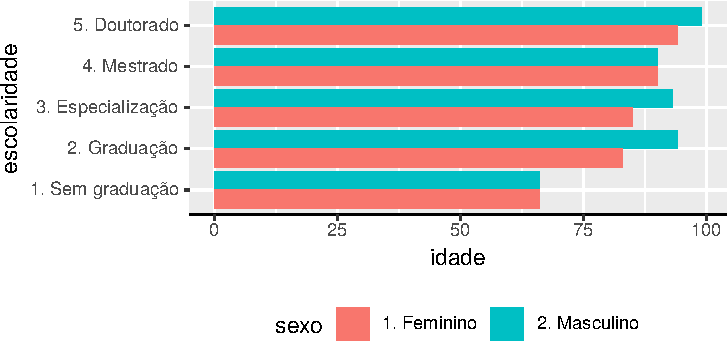
\includegraphics{ebookrnp_files/figure-latex/unnamed-chunk-66-1} 

}

\caption{Colunas de idade vs escolaridade por sexo}\label{fig:unnamed-chunk-66}
\end{figure}

\begin{itemize}
\tightlist
\item
  \textbf{Histogramas agrupados}: Histogramas também são agrupáveis segundo as categorias da variável.
\end{itemize}

\begin{Shaded}
\begin{Highlighting}[]
\NormalTok{p <-}\StringTok{ }\NormalTok{base_docentes }\OperatorTok\StringTok{ }
\StringTok{  }\NormalTok{ggplot2}\OperatorTok{::}\KeywordTok{ggplot}\NormalTok{(}\KeywordTok{aes}\NormalTok{(}\DataTypeTok{x =}\NormalTok{ idade, }\DataTypeTok{fill =}\NormalTok{ escolaridade))}
\NormalTok{p }\OperatorTok{+}\StringTok{ }\NormalTok{ggplot2}\OperatorTok{::}\KeywordTok{theme_gray}\NormalTok{() }\OperatorTok{+}
\StringTok{  }\NormalTok{ggplot2}\OperatorTok{::}\KeywordTok{geom_histogram}\NormalTok{(}\DataTypeTok{bins =} \DecValTok{10}\NormalTok{, }\DataTypeTok{show.legend =} \OtherTok{FALSE}\NormalTok{) }\OperatorTok{+}
\StringTok{  }\NormalTok{ggplot2}\OperatorTok{::}\KeywordTok{facet_wrap}\NormalTok{(.}\OperatorTok{~}\NormalTok{escolaridade)}\OperatorTok{+}
\StringTok{  }\NormalTok{ggplot2}\OperatorTok{::}\KeywordTok{theme}\NormalTok{(}\DataTypeTok{axis.line.x =} \KeywordTok{element_line}\NormalTok{(), }
                 \DataTypeTok{axis.text.x =} \OtherTok{NULL}\NormalTok{, }
                 \DataTypeTok{axis.line.y =} \KeywordTok{element_blank}\NormalTok{())}
\end{Highlighting}
\end{Shaded}

\begin{figure}[H]

{\centering 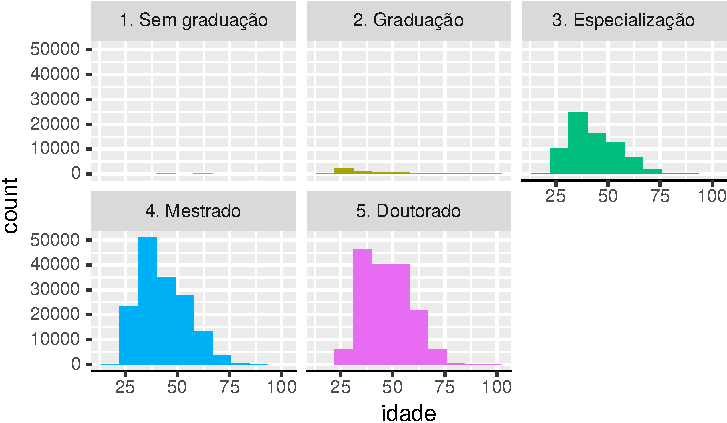
\includegraphics{ebookrnp_files/figure-latex/unnamed-chunk-67-1} 

}

\caption{Histograma de idade vs escolaridade}\label{fig:unnamed-chunk-67}
\end{figure}

\hypertarget{covariancia-e-correlacao}{%
\section{Covariância e correlação}\label{covariancia-e-correlacao}}

Na análise bivariada de variáveis numéricas a covariância e a correlção tem papel fundamental. Ambas se assemelham pelo fato de que medem a direção da relação entre duas variáveis ao longo de seus pontos. As relações mais comuns são \emph{ambas as variáveiscrescem, ambas decrescem, uma decresce e a outra cresce}. A diferença mais significativa entre a coveriância e a correlação é que a primeira oferece um valor absoluto variando de acordo com os dados, graças a isso não tem como estimar a força de uma relação linear. É aí que entra a correlação. Em R a covariância pode ser calculada por \texttt{var()} e \texttt{cov()} e a correção por \texttt{cor()} e se aplica a bases com mais de 2 vriáveis numéricas.

\hypertarget{covariancia}{%
\subsection{Covariância}\label{covariancia}}

O conceito de covariância pode ser aplicado tanto a conjunto de dados como a variáveis aleatórias. Quando aplicada a duas variáveis \(X\) e \(Y\) é expressa por:

\[Cov(X,Y) = \frac {\sum_{i=1}^N(X_i-\bar X)(Y_i - \bar Y)}{N-1}, i=1,..,N\]

Sendo que \(\bar X\) e \(\bar Y\) são as médias das variáveis X e Y.

\BeginKnitrBlock{example}
\protect\hypertarget{exm:unnamed-chunk-68}{}{\label{exm:unnamed-chunk-68} }Vamos calcular a covariância para \texttt{TotalTecnicos} e \texttt{ReceitaPropria}nos dados das IES
\EndKnitrBlock{example}

\begin{Shaded}
\begin{Highlighting}[]
\NormalTok{base_ies }\OperatorTok\StringTok{ }
\StringTok{  }\NormalTok{dplyr}\OperatorTok{::}\KeywordTok{select}\NormalTok{(TotalTecnicos, ReceitaPropria) }\OperatorTok\StringTok{ }
\StringTok{  }\KeywordTok{cov}\NormalTok{() }\OperatorTok\StringTok{ }
\StringTok{  }\NormalTok{knitr}\OperatorTok{::}\KeywordTok{kable}\NormalTok{(}\DataTypeTok{booktabs =} \OtherTok{TRUE}\NormalTok{, }\DataTypeTok{format =}\NormalTok{ tb_formata,}
               \DataTypeTok{caption =} \StringTok{"Análise de covariância"}\NormalTok{) }\OperatorTok\StringTok{ }
\StringTok{  }\NormalTok{kableExtra}\OperatorTok{::}\KeywordTok{kable_styling}\NormalTok{(}\DataTypeTok{latex_options =} \StringTok{"hold_position"}\NormalTok{)}
\end{Highlighting}
\end{Shaded}

\begin{table}[!h]

\caption{\label{tab:unnamed-chunk-69}Análise de covariância}
\centering
\begin{tabular}{lrr}
\toprule
  & TotalTecnicos & ReceitaPropria\\
\midrule
TotalTecnicos & 341089 & 14066046853\\
ReceitaPropria & 14066046853 & 173738053485884832\\
\bottomrule
\end{tabular}
\end{table}

Note que os números são extremamente grandes e tudo que podemos tirar é que a covariância é positiva entre as duas variáveis, mas não conseguimos estimar a força desta relação.

\begin{quote}
Os elementos da diagonal principal da matriz de covariâncias representam a variãncia de cada variável e os valores fora da diagonal são covariâncais.
A matriz é espelhada e para interpretá-la basta ler acima ou abaixo da diagonal principal.
\end{quote}

\hypertarget{correlacao}{%
\subsection{Correlação}\label{correlacao}}

A correlação linear ou de Pearson é uma estatística padronizada que varia de \(-1\) a \(1\) e expressa a relação linear entre duas variáveis numéricas. A correlação é expressa pela letra grega \(\rho\) e é dada pela seguinte expressão matemática:

\[\rho = \frac {\sum_{i=1}^N(X_i-\bar X)(Y_i - \bar Y)}{\sqrt{\sum_{i=1}^N(X_i-\bar X)^2} \times \sqrt{\sum_{i=1}^N(Y_i-\bar Y)^2}}=\frac{Cov(X,Y)}{\sqrt{S^2(X) \times S^2(Y)}}, \\ i=1,..,N\]

Em resumo, esta formula aparentemente complicada diz que a correlação é resultado da covariância dividida pela raiz quadrada do produto das variâncias de cada variável.

\begin{figure}[H]

{\centering 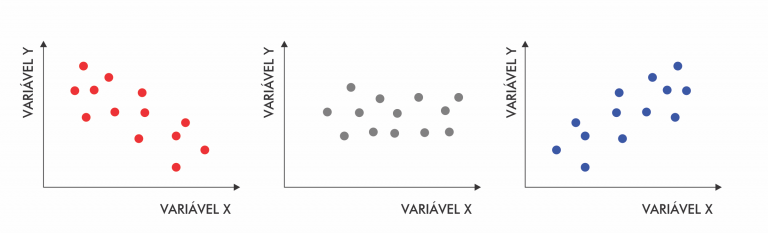
\includegraphics[width=1\linewidth]{../Imagens/ebook_correlacao} 

}

\caption{Tendência da correlação}\label{fig:fig11}
\end{figure}

A figura \ref{fig:fig11} ilustra a relação entre duas variáveis \(X\) e \(Y\). Da esquerda para a direita temos \textbf{correlação linear negativa forte} (tende a \(-1\)), \textbf{correlação fraca} (tende a \(0\)) e \textbf{correlação linear positiva forte} (tende a \(+1\)).

Como regra geral, costuma-se considerar a distribuição expressa na tabela \ref{tab:tab12} para interpretar a correlação. A mesma se aplica para negativa ou positiva bastando apenas dizer estar alerta ao sinal de \(\rho\).

\begin{table}[!h]

\caption{\label{tab:tab12}Interpretação da correlação}
\centering
\begin{tabular}{ll}
\toprule
Faixa & Interprecao\\
\midrule
0.00--0.19 & muito fraca\\
0.20--0.39 & fraca\\
0.40--0.69 & moderada\\
0.70--0.89 & forte\\
0.90--1.00 & muito forte\\
\bottomrule
\end{tabular}
\end{table}

\BeginKnitrBlock{example}
\protect\hypertarget{exm:unnamed-chunk-70}{}{\label{exm:unnamed-chunk-70} }Para o exemplo anterior, determinar e interpretar a correlação entre as duas variáveis. Incluia a variével \texttt{DespesaPesquisa}.
\EndKnitrBlock{example}

\begin{Shaded}
\begin{Highlighting}[]
\NormalTok{base_ies }\OperatorTok\StringTok{ }
\StringTok{  }\NormalTok{dplyr}\OperatorTok{::}\KeywordTok{select}\NormalTok{(TotalTecnicos, ReceitaPropria, DespesaPesquisa) }\OperatorTok\StringTok{ }
\StringTok{  }\KeywordTok{cor}\NormalTok{(}\DataTypeTok{method =} \StringTok{"pearson"}\NormalTok{) }\OperatorTok\StringTok{ }
\StringTok{  }\KeywordTok{round}\NormalTok{(}\DataTypeTok{digits =} \DecValTok{3}\NormalTok{) }\OperatorTok\StringTok{ }
\StringTok{  }\NormalTok{knitr}\OperatorTok{::}\KeywordTok{kable}\NormalTok{(}\DataTypeTok{booktabs =} \OtherTok{TRUE}\NormalTok{, }\DataTypeTok{format =}\NormalTok{ tb_formata,}
               \DataTypeTok{caption =} \StringTok{"Análise de correlação"}\NormalTok{) }\OperatorTok\StringTok{ }
\StringTok{  }\NormalTok{kableExtra}\OperatorTok{::}\KeywordTok{kable_styling}\NormalTok{(}\DataTypeTok{latex_options =} \StringTok{"hold_position"}\NormalTok{)}
\end{Highlighting}
\end{Shaded}

\begin{table}[!h]

\caption{\label{tab:unnamed-chunk-71}Análise de correlação}
\centering
\begin{tabular}{lrrr}
\toprule
  & TotalTecnicos & ReceitaPropria & DespesaPesquisa\\
\midrule
TotalTecnicos & 1.000 & 0.058 & 0.292\\
ReceitaPropria & 0.058 & 1.000 & 0.064\\
DespesaPesquisa & 0.292 & 0.064 & 1.000\\
\bottomrule
\end{tabular}
\end{table}

Note agora que faz mais sentido estimar a força da relação linear entre as variáveis utlizando a correlação. No nosso exemplo, uma correlação linear de \texttt{0.047} entre \texttt{TotalTecnicos} e \texttt{ReceitaPropria} nos diz que a relação linear entre estas duas variáveis é muito fraca. O mesmo se aplica à variável \texttt{DespesaPesquisa} em relação à variável \texttt{TotalTecnicos} com \texttt{0.190}. Estas três variáveis não possuem correlação forte entre si.

\begin{center}\rule{0.5\linewidth}{\linethickness}\end{center}

\cleardoublepage

\hypertarget{appendix-apendice}{%
\appendix \addcontentsline{toc}{chapter}{\appendixname}}


\bibliography{bib/articles.bib,bib/book.bib,bib/packages.bib}

\backmatter
\printindex

\end{document}
